%\documentclass[mat2, tisk]{fmfdelo}
% \documentclass[fin2, tisk]{fmfdelo}
\documentclass[isrm2, tisk]{fmfdelo}

\usepackage[caption = false]{subfig}

\usepackage{listings}
%\lstset{basicstyle=\ttfamily}

\usepackage{xcolor}



\usepackage{color}
\definecolor{lightgray}{rgb}{.9,.9,.9}
\definecolor{darkgray}{rgb}{.4,.4,.4}
\definecolor{purple}{rgb}{0.65, 0.12, 0.82}
\lstdefinelanguage{JavaScript}{
    keywords={abstract, any, as, boolean, break, case, catch, class, console, const, continue, debugger, declare, default, delete, do, else, enum, export, extends, false, finally, for, from, function, get, if, implements, import, in, infer, instanceof, interface, keyof, let, module, namespace, never, new, null, number, object, package, private, protected, public, readonly, require, return,set, static, string, super, switch, symbol, this, throw, true, try, type, typeof, undefined, unique, unknown, var, void, while, with, yield}
    morecomment=[l]{//},
    morecomment=[s]{/*}{*/},
    morestring=[b]',
    morestring=[b]",
    ndkeywords={class, export, boolean, throw, implements, import, this},
    keywordstyle=\color{blue}\bfseries,
    ndkeywordstyle=\color{darkgray}\bfseries,
    identifierstyle=\color{black},
    commentstyle=\color{purple}\ttfamily,
    stringstyle=\color{red}\ttfamily,
    sensitive=true
}

\lstset{
    language=JavaScript,
    backgroundcolor=\color{lightgray},
    extendedchars=true,
    basicstyle=\footnotesize\ttfamily,
    showstringspaces=false,
    showspaces=false,
    numbers=left,
    numberstyle=\footnotesize,
    numbersep=9pt,
    tabsize=2,
    breaklines=true,
    showtabs=false,
    captionpos=b
}


% - ime datoteke z viri (vključno s končnico .bib), če uporabljate BibTeX


% \documentclass[ped, tisk]{fmfdelo}
% Če pobrišete možnost tisk, bodo povezave obarvane,
% na začetku pa ne bo praznih strani po naslovu, …

%%%%%%%%%%%%%%%%%%%%%%%%%%%%%%%%%%%%%%%%%%%%%%%%%%%%%%%%%%%%%%%%%%%%%%%%%%%%%%%
% METAPODATKI
%%%%%%%%%%%%%%%%%%%%%%%%%%%%%%%%%%%%%%%%%%%%%%%%%%%%%%%%%%%%%%%%%%%%%%%%%%%%%%%

% - vaše ime
\avtor{Kevin Štampar}

% - naslov dela v slovenščini
\naslov{Orodje za grafični prikaz lastnosti Bézierjevih in PH krivulj}

% - naslov dela v angleščini
\title{Tool for graphical representation of properties of Bézier and PH curves}

% - ime mentorja/mentorice s polnim nazivom:
%   - doc.~dr.~Ime Priimek
%   - izr.~prof.~dr.~Ime Priimek
%   - prof.~dr.~Ime Priimek
%   za druge variante uporabite ustrezne ukaze
\mentor{prof.~dr.~Emil Žagar}
% \somentor{...}
% \mentorica{...}
% \somentorica{...}
% \mentorja{...}{...}
% \somentorja{...}{...}
% \mentorici{...}{...}
% \somentorici{...}{...}

% - leto magisterija
\letnica{2024}

% - povzetek v slovenščini
%   V povzetku na kratko opišite vsebinske rezultate dela. Sem ne sodi razlaga
%   organizacije dela, torej v katerem razdelku je kaj, pač pa le opis vsebine.
% Delo je močno podprto s slikovnim gradivom, ki je nastalo s pomočjo orodja.
\povzetek{V magistrskem delu obravnavamo Bézierjeve krivulje, racionalne Bézierjeve krivulje, zlepke Bézierjevih krivulj ter PH krivulje.
Skozi delo predstavimo njihove lastnosti, ki so ključne za rabo v sistemih za računalniško podprto načrtovanje (ang.\ computer-aided design, okrajš.\ CAD) in sistemih za računalniško podprto geometrijsko oblikovanje (ang.\ computer-aided geometric design, okrajš.\ CAGD) ter algoritme, ki njihovo rabo v takšnih sistemih omogočajo.
Predstavimo tudi orodje za grafični prikaz lastnosti prej naštetih krivulj - Bezeg.
Ogledamo si njegove funkcionalnosti in pokažemo osnovne ideje za tem, kako je orodje implementirano in kako so v orodju implementirane prej naštete krivulje.
}

% - povzetek v angleščini
\abstract{An abstract of the work is written here. This includes a short description of
the content and not the structure of your work.}

% - klasifikacijske oznake, ločene z vejicami
%   Oznake, ki opisujejo področje dela, so dostopne na strani https://www.ams.org/msc/
\klasifikacija{74B05, 65N99}

% - ključne besede, ki nastopajo v delu, ločene s \sep
\kljucnebesede{integracija\sep kompleks}

% - angleški prevod ključnih besed
\keywords{integration\sep complex} % angleški prevod ključnih besed

% - neobvezna zahvala
\zahvala{
    Zahvaljujem se mentorju za zelo sproščen odnos!
}

% - program dela, ki ga napiše mentor z osnovno literaturo
\programdela{
    V okviru magistrskega dela opišite Bézierjeve krivulje in krivulje s pitagorejskim hodografom (PH krivulje).
    Predstavitev njihove osnovne lastnosti in izdelajte spletno orodje za njihovo vizualizacijo.
}

\osnovnaliteratura{
% Literatura mora biti tukaj posebej samostojno navedena (po pomembnosti) in ne
% le citirana. V tem razdelku literature ne oštevilčimo po svoje, ampak uporabljamo
% ukaz \vnosliterature, v katerega vpišemo citat
%    \vnosliterature{24ac2b10-13c2-3e17-bc91-5f7366bf076c}
    \vnosliterature{farouki}
}

% - ime datoteke z viri (vključno s končnico .bib), če uporabljate BibTeX
\literatura{literatura.bib}

%%%%%%%%%%%%%%%%%%%%%%%%%%%%%%%%%%%%%%%%%%%%%%%%%%%%%%%%%%%%%%%%%%%%%%%%%%%%%%%
% DODATNE DEFINICIJE
%%%%%%%%%%%%%%%%%%%%%%%%%%%%%%%%%%%%%%%%%%%%%%%%%%%%%%%%%%%%%%%%%%%%%%%%%%%%%%%

% naložite dodatne pakete, ki jih potrebujete
\usepackage{units}        % fizikalne enote kot \unit[12]{kg} s polovico nedeljivega presledka, glej primer v kodi
\usepackage{graphicx}     % za slike
% \usepackage{tikz}
% VEČ ZANIMIVIH PAKETOV
% \usepackage{array}      % več možnosti za tabele
% \usepackage[list=true,listformat=simple]{subcaption}  % več kot ena slika na figure, omogoči slika 1a, slika 1b
% \usepackage[all]{xy}    % diagrami
% \usepackage{doi}        % za clickable DOI entrye v bibliografiji
\usepackage{enumitem}     % več možnosti za sezname

% Za barvanje source kode
% \usepackage{minted}
% \renewcommand\listingscaption{Program}

% Za pisanje psevdokode
\usepackage{algpseudocode}  % za psevdokodo
\usepackage{algorithm}
\usepackage{algorithmicx}
\usepackage{mathtools}
\usepackage{hyperref}
\usepackage{graphics}
\usepackage{titlesec}
\newcommand{\sectionbreak}{\clearpage}
\floatname{algorithm}{Algoritem}
\renewcommand{\listalgorithmname}{Kazalo algoritmov}

% deklarirajte vse matematične operatorje, da jih bo LaTeX pravilno stavil
% \DeclareMathOperator{\...}{...}

% vstavite svoje definicije ...
\newcommand{\R}{\mathbb R}
\newcommand{\N}{\mathbb N}
\newcommand{\Z}{\mathbb Z}
% Lahko se zgodi, da je ukaz \C definiral že paket hyperref,
% zato dobite napako: Command \C already defined.
% V tem primeru namesto ukaza \newcommand uporabite \renewcommand
\newcommand{\C}{\mathbb C}
\newcommand{\Q}{\mathbb Q}
\newcommand{\Pn}{\mathbb P_n}
\newcommand{\p}{\mathbf{p}}
\newcommand{\B}{\mathbf{B}}

\newcommand{\groupimagewidth}{0.28\textwidth}
%0.27 = 33 strani

%Bernstein
\newcommand{\bernsteinbase}[3]{\binom{#1}{#2}t^{#1}(1-t)^{#2}}
\newcommand{\bernstein}[2]{\binom{#1}{#2}t^{#2}(1-t)^{#1-#2}}
\newcommand{\lilb}[2]{B_{#1}^{#2}(t)}
\newcommand{\bigb}[1]{B_{#1}(t)}
\newcommand{\bigbb}[1]{\textbf{B}_{#1}(t)}
\newcommand{\bigbbod}[2]{\textbf{B}_{#1}(#2)}
\newcommand{\bigbbt}{\textbf{B}(t)}
\newcommand{\bigbo}[1]{B'_{#1}(t)}
\newcommand{\bernsteinsum}[2]{\sum_{#1=0}^{#2} \beta_{#1}\lilb{#1}{#2}}
\newcommand{\bernsteinsump}[2]{\sum_{#1=0}^{#2} \p_{#1}\lilb{#1}{#2}}
\newcommand{\bernsteinsumtri}[3]{\sum_{#1=0}^{#2} #3_{#1}\lilb{#1}{#2}}
\newcommand{\bernsteinsumtritri}[3]{\sum_{#1=0}^{#2} #3\lilb{#1}{#2}}
\newcommand{\bernsteinsumtridva}[2]{\sum_{#1=0}^{#2} \lilb{#1}{#2}}

\newcommand{\bsum}{\bernsteinsum{i}{n}}

% Komentarji znotraj vsebine
\newcommand{\mycomment}[1]{\textbf{\textcolor{red}{#1}}}
\newcommand{\missingref}[1]{\mycomment{referenca-#1}}


%%%%%%%%%%%%%%%%%%%%%%%%%%%%%%%%%%%%%%%%%%%%%%%%%%%%%%%%%%%%%%%%%%%%%%%%%%%%%%%
% ZAČETEK VSEBINE
%%%%%%%%%%%%%%%%%%%%%%%%%%%%%%%%%%%%%%%%%%%%%%%%%%%%%%%%%%%%%%%%%%%%%%%%%%%%%%%

\begin{document}

    \section{Uvod}
%    Napišite kratek zgodovinski in matematični uvod. Pojasnite motivacijo za problem, kje
%    nastopa, kje vse je bil obravnavan.
    Za namene računalniško podprtega geometrijskega oblikovanja (ang.\ computer-aided geometric design, okrajš.\ CAGD) v avtoindustriji, sta v zgodnjih šestdesetih letih prejšnjega stoletja francoska inženirja Paul de Casteljau in Pierre Bézier vzporedno uvedla Bézierjeve krivulje.
    To so parametrično podane krivulje, ki temeljijo na kontrolnih točkah, preko katerih uporabnik CAGD sistema s krivuljo upravlja.
    Zaradi enostavnega upravljanja z njimi, se je njihova raba razširila tudi v sisteme za računalniško podprto geometrijsko oblikovanje izven avtoindustrije, ter sisteme za računalniško podprto načrtovanje (ang.\ computer-aided design, okrajš.\ CAD).
    Danes se o Bézierjevih krivuljah (in njihovih variacijah) učimo tudi na faksu, kjer se je pojavila želja po orodju, s katerim bi lahko predavatelji grafično prikazovali njihove lastnosti.
    Cilj magistrskega dela je krivulje opisati, ter takšno orodje tudi izdelati.
    V času pisanja je orodje že izdelano, zato je delo bogato s slikovnim gradivom, ki je bilo ustvarjeno z njim.

%    Na koncu opišite tudi organizacijo dela -- kaj je v
%    katerem razdelku.
    Delo bomo začeli s poglavjem o Bézierjevih krivuljah, kjer bomo najprej spoznali Bernsteinove bazne polinome.
    Predstavili bomo nekaj njihovih ključnih lastnosti, nato pa bomo z njihovo pomočjo Bézierjeve krivulje tudi vpeljali.
    Pokazali bomo nekaj osnovnih lastnosti krivulj, nadaljevali pa bomo z De Casteljaujevim algoritmom, ki je ključen za stabilno računanje točk Bézierjeve krivulje.
    Podrobneje si bomo ogledali lastnosti subdivizije, ekstrapolacije ter višanja stopnje Bézierjeve krivulje, zaključili pa bomo z odvodi Bézierjeve krivulje, ki bodo pomembni pri tvorjenju zlepkov Bézierjevih krivulj v šestem poglavju.

    V tretjem poglavju se bomo posvečali racionalnim Bézierjevim krivuljam.
    Ogledali si bomo delovanje uteži racionalne Bézierjeve krivulje in število dodatnih prostih parametrov, ki jih dobimo v primerjavi s polinomskimi Bézierjevimi krivuljami.
    Pokazali bomo racionalni De Casteljaujev algoritem, ki je razširitev De Casteljaujevega algoritma iz drugega poglavja.
    Nato pa bomo predstavili še Farinove točke, ki uporabniku CAGD sistema nudijo naravno kontrolo nad utežmi racionalne Bézierjeve krivulje.

    Četrto poglavje je namenjeno zlepkom Bézierjevih krivulj.
    Najprej bomo zlepke krivulj definirali, nato pa izpeljali pogoje gladkosti za zlepke Bézierjevih krivulj.
    Predstavili bomo koncept geometrijske zveznosti in izpeljali nekaj pogojev za različne stopnje geometrijske zveznosti.
    Proti koncu poglavja bomo podali nekaj algoritmov za konstrukcijo zlepkov Bézierjevih krivulj, zaključili pa bomo s posebnimi tipi parametrizacij.

    V naslednjem poglavju predstavimo krivulje s pitagorejskim hodografom (PH krivulje).
    Najprej pokažemo, da nelinearne polinomske krivulje ne premorejo konstantne parametrične hitrosti.
    Kot alternativo predstavimo PH krivulje, ki imajo polinomsko parametrično hitrost.
    S pomočjo Bernsteinovih polinomov nato izrazimo kontrolne točke Bézierjevih PH krivulj stopnje $3$ in $5$.
    Izpeljemo parametrično hitrost Bézierjevih PH krivulj, ki jo nato uporabimo pri iskanju približka za enakomerno parametrizacijo.
    Pokažemo tudi, da so funkcije tangente, normale in ukrivljenosti PH krivulje racionalne funkcije in kot posledico izrazimo odmik krivulje Bézierjeve PH krivulje kot racionalno Bézierjevo krivuljo.
    V zaključku poglavja izrazimo še kontrolne točke kubične in kvintične Bézierjeve PH krivulje s kompleksnimi števili.

    V šestem poglavju se posvetimo spletnemu orodju (Bezeg) za grafični prikaz lastnosti krivulj, ki je nastalo v okviru tega dela.
    V prvem delu poglavja predstavimo uporabniški vmesnik orodja in njegove funkcionalnosti.
    Drugi del pa je namenjen predstavitvi implementacije orodja, kjer predstavimo arhitekturo aplikacije in opišemo osnovne ideje za njo, ter podamo nekaj primerov kode iz implementacije.


    \section{Bézierjeve krivulje}\label{sec:bezierjeve-krivulje}

    \subsection{Bernsteinovi bazni polinomi}\label{subsec:bernsteinovi-polinomi}
    V tem podrazdelku bomo predstavili Bernsteinove bazne polinome in nekaj njihovih lastnosti, ki bodo ključne pri vpeljavi Bézierjevih krivulj.
    Začnimo z njihovo definicijo.
    \begin{definicija}
        \label{def:bernstein}
        Za nenegativna cela števila $n$ je $i$-ti \textit{Bernsteinov bazni polinom} podan s predpisom \[B_i^n(t)\coloneqq\bernstein{n}{i},\quad i = 0,1\ldots,n.\]
    \end{definicija}
    % V definiciji Bernsteinovega polinoma smo uporabili le bazne polinome z indeksi $i=0,\ldots,n$.
    \begin{opomba}
        Kjer je potrebno, lahko definicijo razširimo tudi na indekse $i>n$, oziroma $i<0$.
        Iz definicije potem sledi $B_i^n(t)=0$.
    \end{opomba}
    \noindent Pri določeni stopnji $n$ je Bernsteinovih baznih polinomov torej $n+1$.
    Brez dokaza povejmo, da so linearno neodvisni in zato tvorijo bazo prostora polinomov stopnje manjše ali enake $n$ ($\mathbb{P}_n$).
    Takšni bazi pravimo \textit{Bernsteinova baza}, polinomu, izraženemu v njej, pa pravimo \textit{Bernsteinov polinom}.
    \begin{primer}
        \label{primer:bernsteinovi}
        Za primer si bomo ogledali Bernsteinove bazne polinome stopenj $n=0,1,2,3$.
        Pri stopnji $0$ imamo konstantni polinom s funkcijskim predpisom $B_{0}^{0}(t) = 1$.
        Za stopnjo $1$ dobimo dva polinoma s funkcijskima predpisoma $B_{0}^{1}(t) = 1-t$ in $B_{1}^{1}(t) = t$.
        Funkcijski predpisi kvadratnih in kubičnih Bernsteinovih baznih polinomov pa so:
        \begin{align*}
            &B_{0}^{2}(t) = (1-t)^2,\quad B_{1}^{2}(t) = 2t(1-t),\quad B_{2}^{2}(t) = t^2,  \\
            &B_{0}^{3}(t) = (1-t)^3,\quad B_{1}^{3}(t) = 3t(1-t)^2,\quad B_{2}^{2}(t) = 3t^2(1-t),\quad B_{3}^{3}(t) = t^3.
        \end{align*}
        Grafe polinomov iz primera si lahko ogledamo na sliki~\ref{fig:bernstein-base}.
    \end{primer}
    \begin{figure}[h!]
        \captionsetup[subfigure]{labelformat=empty}
        \centering
        \subfloat[$n=0$]{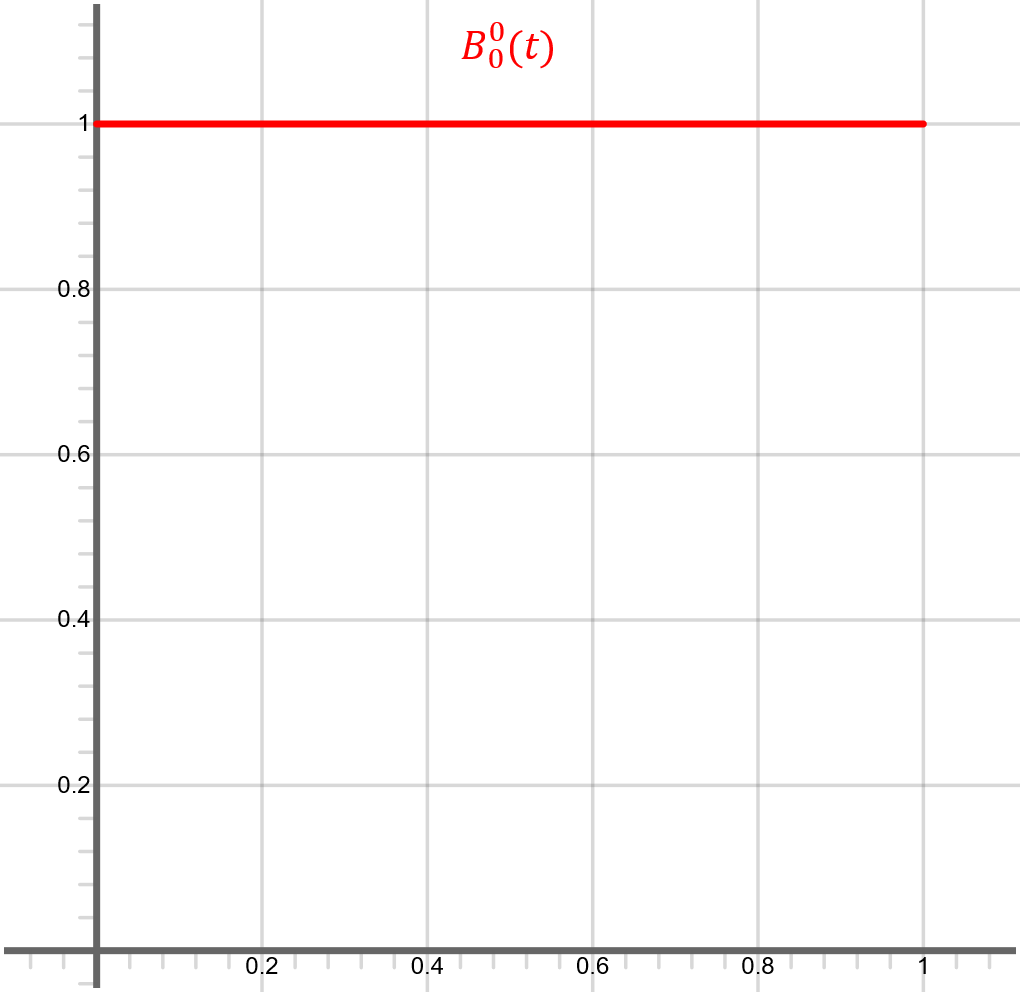
\includegraphics[width = \groupimagewidth]{images/bernstein-0}}
        \qquad
        \subfloat[$n=1$]{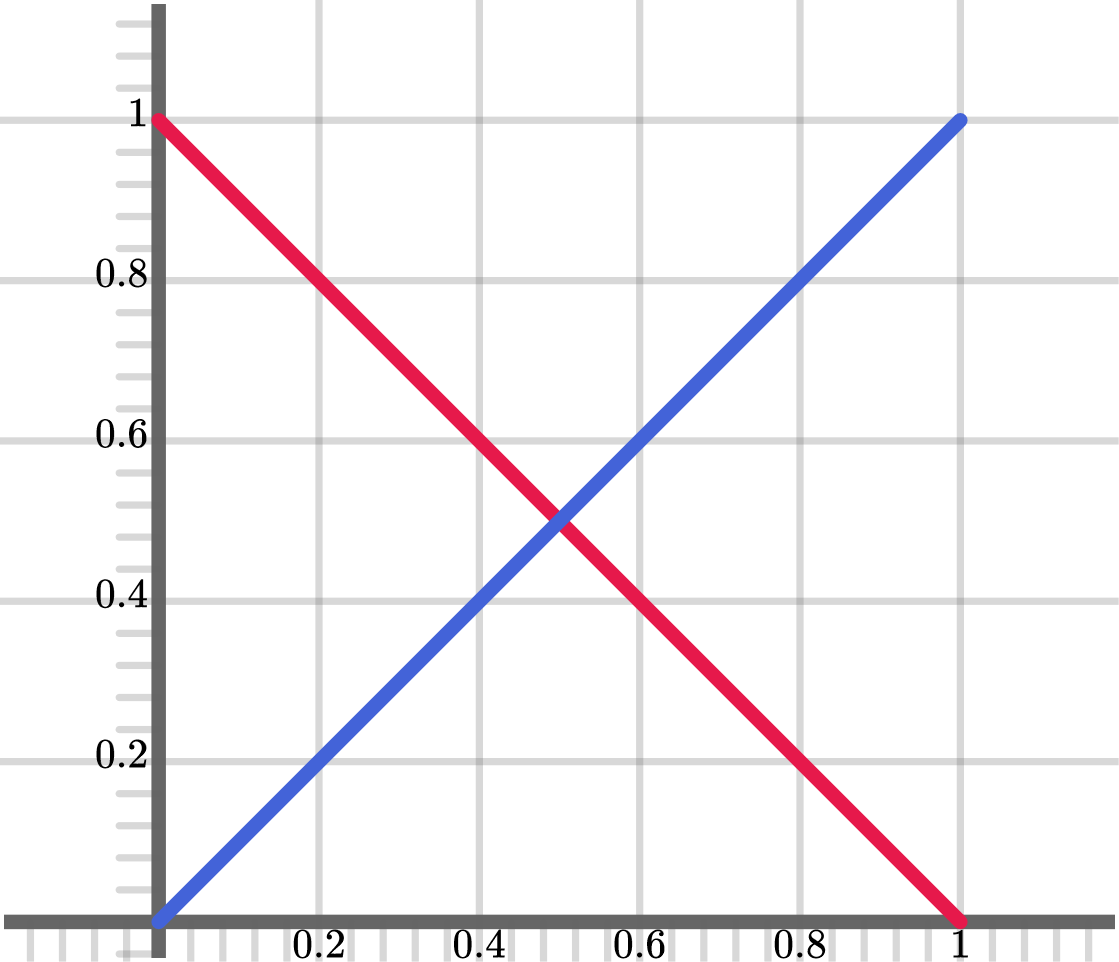
\includegraphics[width = \groupimagewidth]{images/bernstein-1}} \\
        \subfloat[$n=2$]{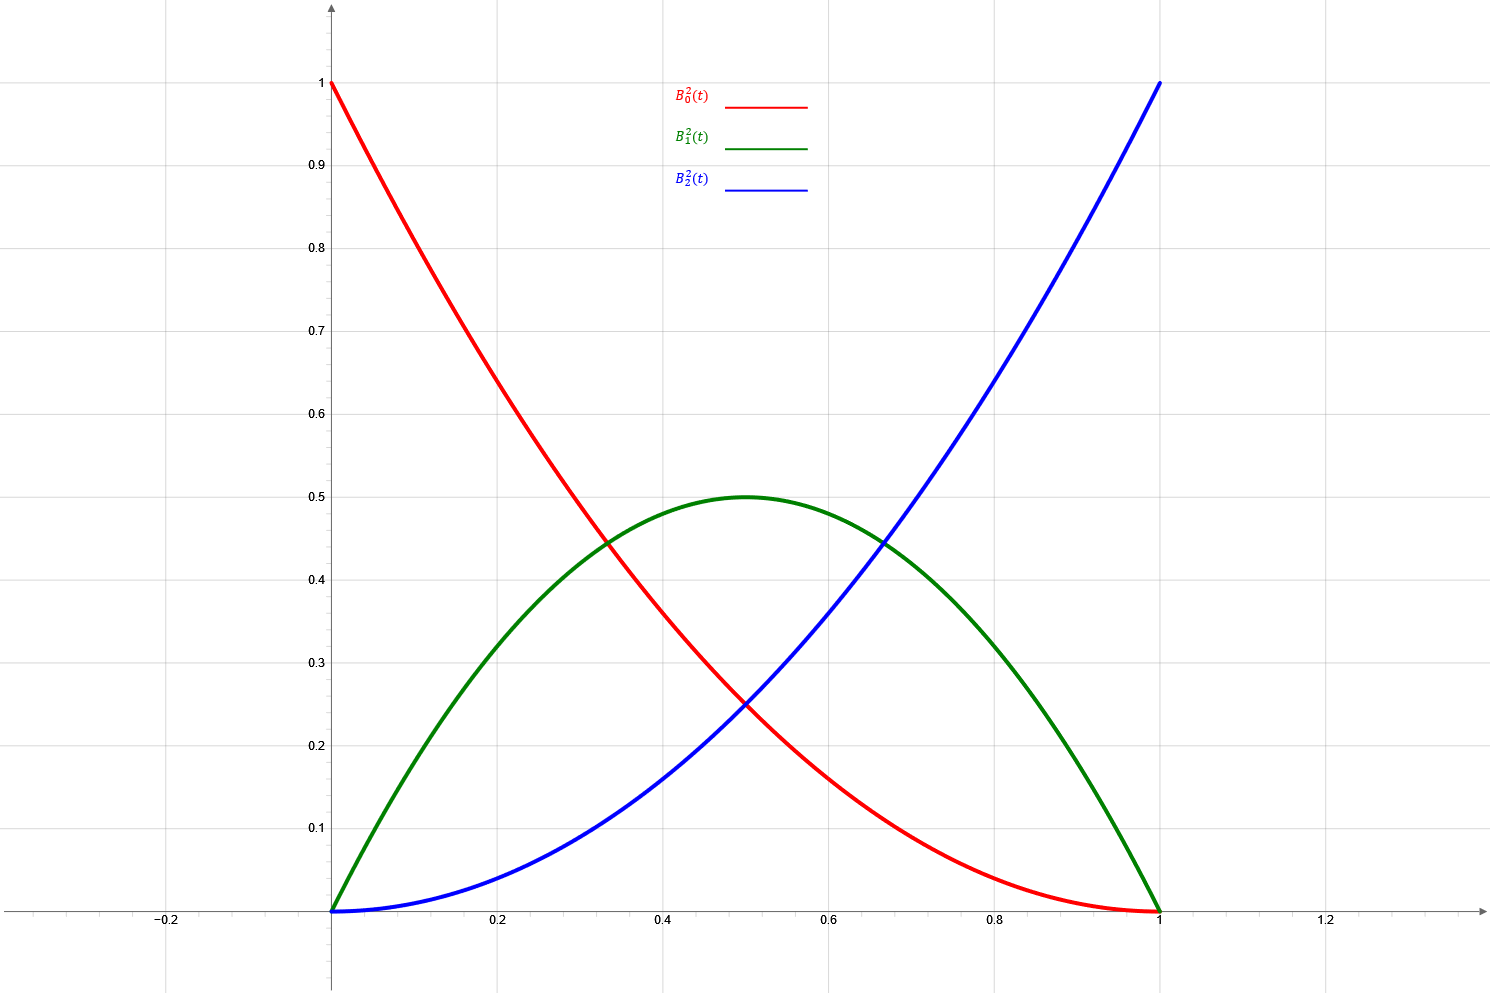
\includegraphics[width = \groupimagewidth]{images/bernstein-2}}
        \qquad
        \subfloat[$n=3$]{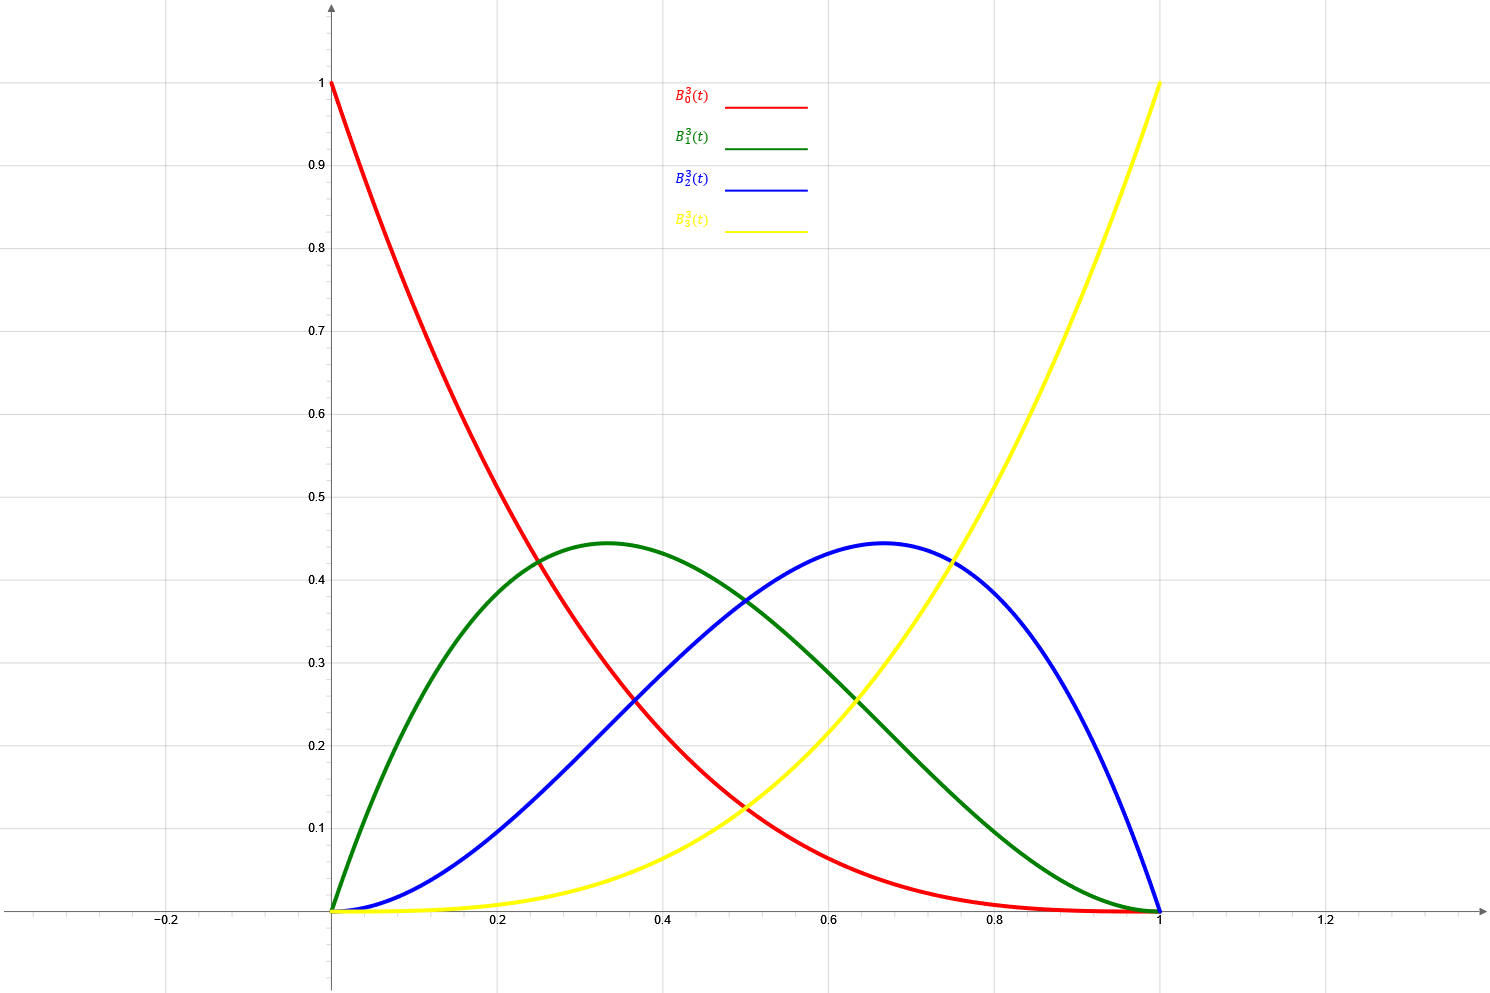
\includegraphics[width = \groupimagewidth]{images/bernstein-3}}
        \caption{Bernsteinovi bazni polinomi stopenj $n=0,1,2,3$.}
        \label{fig:bernstein-base}
    \end{figure}
    Brez dokaza v naslednjem izreku naštejmo nekaj osnovnih lastnosti Bernsteinovih baznih polinomov.
    \begin{izrek}
        Za Bernsteinove bazne polinome $B_i^n$ veljajo naslednje lastnosti.
        \label{izrek:bernsteinovi_lastnosti}
        \begin{enumerate}
            \item So nenegativni na intervalu $[0,1]$.\label{izrek:bernsteinovi_lastnosti:pozitivnost}
            \item $B_i^n(0) = \delta_{i,0}$ in $B_i^n(1) = \delta_{i,n}$, kjer je $\delta_{i,j} = \begin{cases}
                                                                                                      1, & i=j, \\
                                                                                                      0, & 1\neq j.
            \end{cases}$
            \item So simetrični, tj.\ $B_i^n(1-t) = B^n_{n-i}(t)$, $t\in\R$. \label{izrek:bernsteinovi_lastnosti:simetrija}
            \item Tvorijo razčlenitev enote, tj.\  $\sum_{i=0}^{n}B_{i}^{n}(t) = 1$, $t\in\R$.\label{izrek:bernsteinovi_lastnosti:enota}
        \end{enumerate}
    \end{izrek}
%    \begin{dokaz}
%        Lastnost (1) očitno izhaja iz lastnosti binomskega simbola, lastnost (2) pa iz definicije.
%        Dokažimo simetričnost in razčlenitev enote.\\
%        \noindent(3) Namesto spremenljivke $t$ v enačbo za bernsteinov bazni polinom $B_i^n(t)$ vstavimo izraz $1-t$ in uporabimo lastnost binomskega simbola $\binom{n}{i} = \binom{n}{n-i}$, dobimo
%        \[B_i^n(1-t) = \binom{n}{i}(1-t)^i(1-(1-t))^{n-i} =  \binom{n}{n-i}(1-t)^it^{n-i} = B^{n-i}_{i}(t).\]
%        \noindent(5) Za $1 = 1^n = (1-t+t)^n = ((1-t) + t)^n$ uporabimo binomski izrek, dobimo
%        \[\left((1-t) + t\right)^n = \sum_{i=0}^{n}\bernstein{n}{i} = \sum_{i=0}^n B_i^n(t).\]
%    \end{dokaz}
    \noindent Prve tri lastnosti iz izreka lahko opazimo na že prej omenjeni sliki~\ref{fig:bernstein-base}.
    Četrto lastnost pa je moč opaziti na sliki~\ref{fig:bernstein-base-sum}, kjer so prikazani naloženi ploščinski grafikoni Bernsteinovih baznih polinomov. % za stopnje $n=0,1,2,3$.
    Količina barve pri določenem parametru $t\in[0,1]$ pove, koliko pripadajoč polinom $B_i^n$ prispeva k razčlenitvi enote.
    \begin{figure}[h]
        \captionsetup[subfigure]{labelformat=empty}
        \centering
        \subfloat[$n=0$]{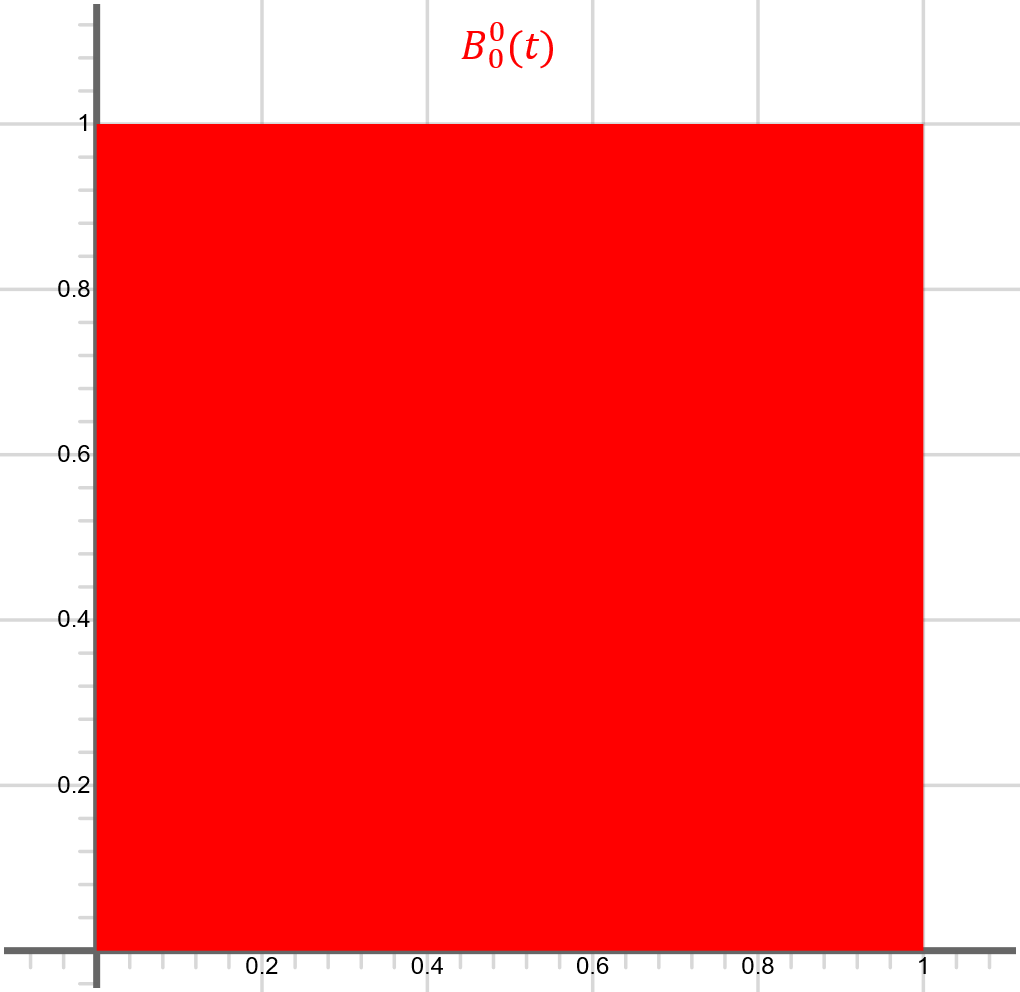
\includegraphics[width = \groupimagewidth]{images/bernstein-sum-0}}
        \qquad
        \subfloat[$n=1$]{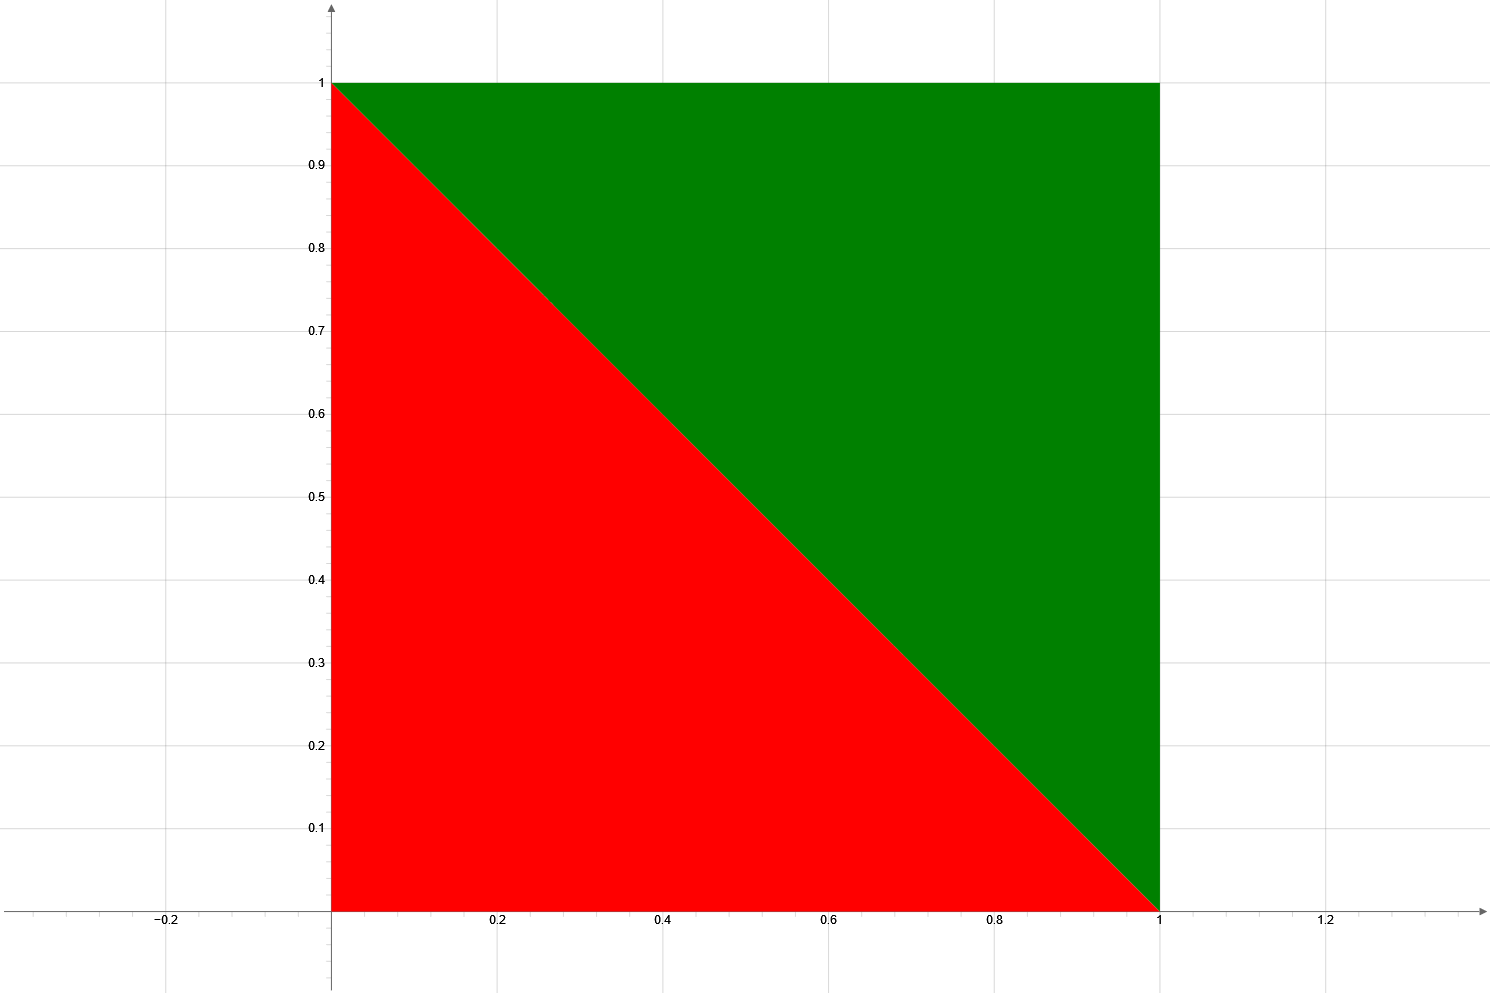
\includegraphics[width = \groupimagewidth]{images/bernstein-sum-1}} \\
        \subfloat[$n=2$]{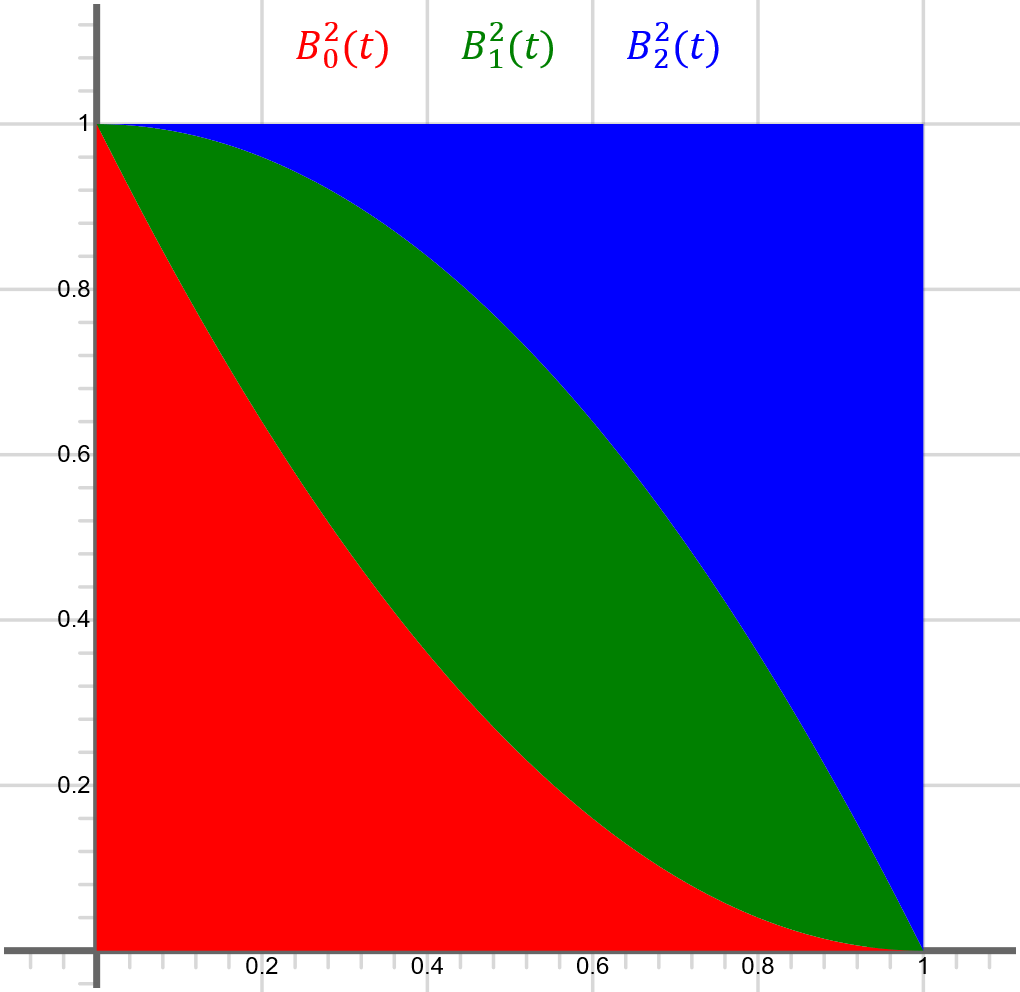
\includegraphics[width = \groupimagewidth]{images/bernstein-sum-2}}
        \qquad
        \subfloat[$n=3$]{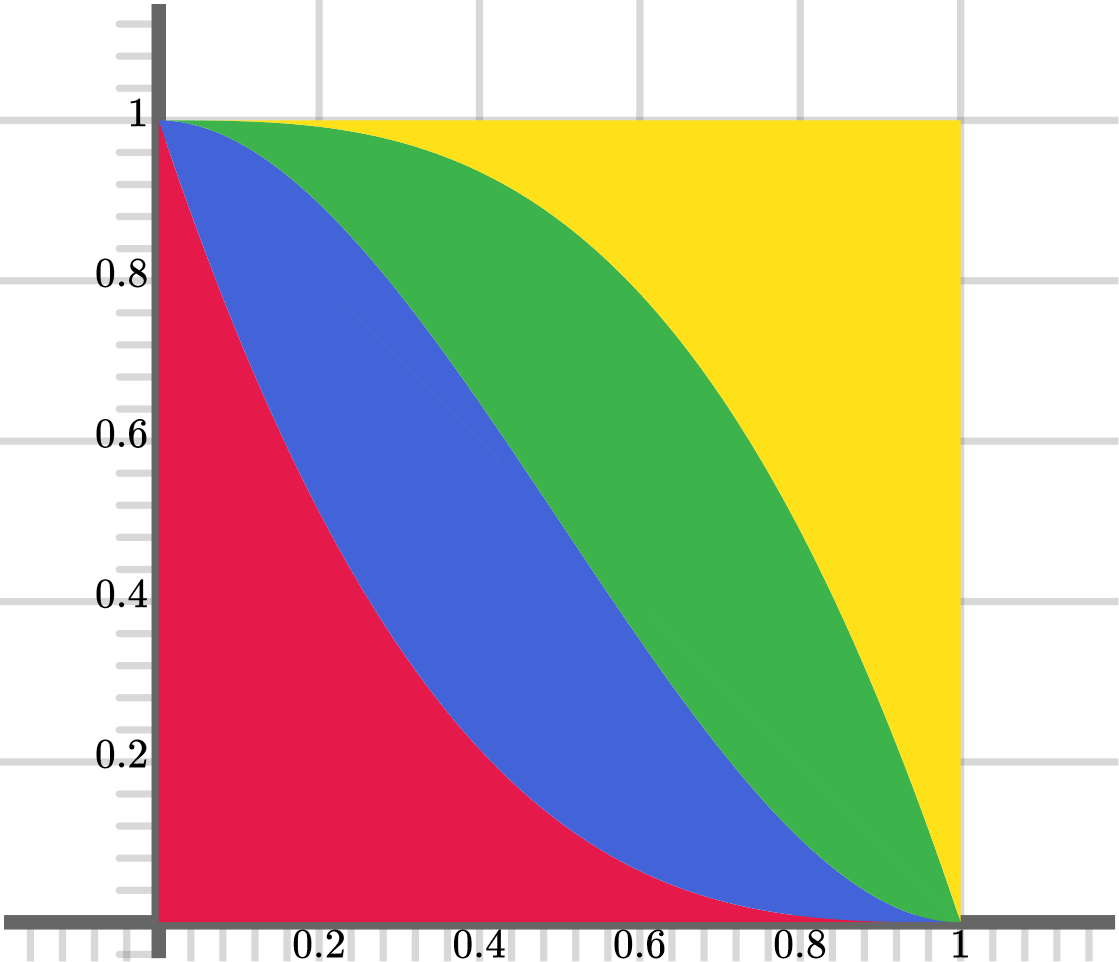
\includegraphics[width = \groupimagewidth]{images/bernstein-sum-3}}
        \caption{Naloženi ploščinski grafikoni Bernsteinovih baznih polinomov.}
        \label{fig:bernstein-base-sum}
    \end{figure}

    S sledečim izrekom podamo rekurzivno zvezo za računanje vrednosti Bernsteinovih baznih polinomov.
    \begin{izrek}
        \label{izrek:bernsteinovi_lastnosti:rekruzija}
        Za Bernsteinove bazne polinome stopnje $n\geq1$ velja rekurzivna zveza
        \[B_i^n(t) = (1-t)B_i^{n-1}(t) + tB_{i-1}^{n-1}(t),\ t\in\R.\]
    \end{izrek}
    \noindent Izrek je enostavno dokazati s pomočjo indukcije, zato bomo dokaz izpustili.
%    Rekurzivno zvezo dokažimo z indukcijo.
%    \begin{dokaz}
%        Za $n=1$ zveza drži, saj iz nje dobimo $B_i^1(t) = (1-t)B_i^{0}(t) + tB_{i-1}^{0}(t)$ oziroma $B_0^1(t) = (1-t)$ in $B_1^1(t) = t$.
%        Za indukcijski korak pa desni del rekurzivne zveze manipuliramo, da pridemo do levega
%        \begin{align*}
%        (1-t)
%            B_i^{n-1}(t) + tB_{i-1}^{n-1}(t) &= \binom{n-1}{i}t^{i}(1-t)^{n-i} + \binom{n-1}{i-1}t^{i}(1-t)^{n-i}  \\
%            &\stackrel{(1)}{=} \binom{n}{i}t^{i}(1-t)^{n-i} = B_i^n(t),
%        \end{align*}
%        kjer smo pri enakosti (1) uporabili lastnost binomskega simbola $\binom{n-1}{i} + \binom{n-1}{i-1} = \binom{n}{i}.$
%    \end{dokaz}
    V kasnejših razdelkih bomo potrebovali tudi odvode in integrale Bernsteinovih baznih polinomov.
    Ker Bernsteinovi bazni polinomi stopnje $n$ tvorijo bazo prostora $\mathbb{P}_n$, lahko njihove odvode izrazimo v Bernsteinovi bazi dimenzije $n-1$.
    Z nekaj računanja pridemo do sledečega rezultata.
    \begin{izrek}
        \label{izrek:bernstein-odvod}
        Za odvode Bernsteinovih baznih polinomov velja zveza
        \[B_{i}^{n\prime}=n(B_{i-1}^{n-1} - B_{i}^{n-1}).\]
    \end{izrek}
    \noindent S pomočjo prejšnjega izreka in indukcije pa pridemo do izreka za integrale Bernsteinovih baznih polinomov.
    \begin{izrek}
        \label{izrek:bernstein-integral}
        Nedoločeni integrali Bernsteinovih baznih polinomov so
        \[\int B_{i}^{n}(t)dt= \frac{1}{n+1} \sum_{k=1}^{n-i+1}  B_{i+k}^{n+1}(t) + C,\quad C\in\R. \]
    \end{izrek}
%    \begin{dokaz}
%        Bernsteinov bazni polinom najprej odvajamo da dobimo
%        \begin{align*}
%            B_{i}^{n\prime}(t) &=\binom{n}{i}\left(it^{i-1}(1-t)^{n-i} - (n-i) t^i(1-t)^{n-i-1} \right) \\
%            &=\binom{n}{i}it^{i-1}(1-t)^{n-i} - \binom{n}{i}(n-i) t^i(1-t)^{n-i-1}.
%        \end{align*}
%        Nato v zgornje vstavimo binomski zvezi $\binom{n}{i}i = \frac{n!i}{(n-i)i!} =  \frac{n(n-1)!}{(n-i)(i-1)!} = n\binom{n-1}{i-1}$ in $\binom{n}{i}(n-i) = \frac{n!(n-i)}{(n-i)!}  = \frac{n(n-1)!}{(n-i-1)!} =n\binom{n-1}{i}$ in dobimo željeno.
%    \end{dokaz}
    Za konec podrazdelka izpeljimo še formulo za zmnožek dveh Bernsteinovih polinomov.
    \begin{izrek}
        \label{izrek:bernstein-multiplication}
        Naj bosta $f$ in $g$ Bernsteinova polinoma definirana kot $f=\sum_{i=0}^{m}\alpha_iB_i^m$ in $g=\sum_{i=0}^{n}\beta_iB_i^n$.
        Potem za njun zmnožek velja
        \[ fg = \sum_{i=0}^{m+n}\left(\sum_{j=\max(0,i-n)}^{\min(m,i)} \frac{\binom{m}{j}\binom{n}{i-j}}{\binom{m+n}{i}} \alpha_i\beta_{i-j} \right)B_{i}^{m+n}.\]
    \end{izrek}
    \begin{dokaz}
        Naj bosta $f$ in $g$ Bernsteinova polinoma iz predpostavk izreka.
        Polinoma zmnožimo in dobimo
        \[fg =\sum_{i=0}^{m}\alpha_iB_{i}^{m}\sum_{j=0}^{n}\beta_jB_{j}^{n} = \sum_{i=0}^{m+n}\sum_{l=0}^i \alpha_lB_{l}^{m}\beta_{i-l}B_{i-l}^{n}. \]
        V zadnji izraz vstavimo funkcijske predpise Bernsteinovih baznih polinomov, ga poenostavimo in dobimo
        %&= \sum_{i=0}^{m+n}\sum_{l=0}^i \alpha_l \binom{m}{l}t^{l}(1-t)^{m-l} \beta_{i-l} \binom{n}{i-l}t^{i-l}(1-t)^{n-i+l} \\
        \[\sum_{i=0}^{m+n}\sum_{l=0}^i \alpha_l \beta_{i-l} \binom{m}{l}\binom{n}{i-l}t^{i}(1-t)^{m+n-i}.\]
        Slednje lahko z izpostavitvijo binoma $\binom{m+n}{i}$ predstavimo v Bernsteinovi bazi kot
        \[\sum_{i=0}^{m+n} \left(\sum_{l=0}^i  \alpha_l \beta_{i-l}\frac{\binom{m}{l}\binom{n}{i-l}}{\binom{m+n}{i}}\right) B_{i}^{m+n}.\]
        V primerih, ko je $l>m$ ali $i-l>n$, imamo v števcu ulomka $0$, kar privede do zapisa iz izreka.
    \end{dokaz}

    \subsection{Večdimenzionalne oznake}
    Da bodo zapisi v sledečih razdelkih bolj pregledni, bomo uvedli večdimenzionalne oznake.
%    Večdimenzionalnost bomo ponazarjali z odebelitvijo črke.
    Točke v večdimenzionalnem prostoru bomo označili z odebeljenimi črkami, na primer $\mathbf{x}=(x_0,x_1,\dots,x_n)\in\R^{n+1}$.
    Podobno bomo odebelili črke funkcij, ki v večdimenzionalni prostor slikajo, na primer $\mathbf{f}:\R\to\R^{n+1}$.
%    Tako bomo večdimenzionalnost točke $x\in\R^{n+1}$ označili z $\mathbf{x}=(x_0,x_1,\dots,x_n)$, večdimenzionalnost funkcije $f:\R\to\R^{n+1}$ pa z $\mathbf{f}=\left( f_0,f_1,\dots,f_n\right)$.

    \subsection{Bézierjeve krivulje}
    Če v Bernsteinovem polinomu skalarne koeficiente zamenjamo s točkami, dobimo predpis parametrizacije Bézierjeve krivulje.
    \begin{definicija}
        Bézierjeva krivulja $\mathbf{B}: [0,1]\to \R^d$ stopnje $n\in\N$ je polinomska krivulja podana s točkami $\p_i\in\R^d$,  $i=0,1,\ldots,n$, in parametrizacijo
        \[\mathbf{B}(t)=\bernsteinsump{i}{n}.\]
        Točkam $\p_i$ pravimo \textit{kontrolne točke}.
        Če zaporedne kontrolne točke povežemo, dobimo \textit{kontrolni poligon}.
    \end{definicija}
    \begin{opomba}
        \label{opomba:dim-0}
        Kjer je potrebno, lahko definicijo razširimo tudi na stopnjo $n=0$.
        Iz zgornje parametrizacije potem sledi $\mathbf{B}(t)=\p_0$.
    \end{opomba}
    \begin{opomba}
        Pri slikovnem gradivu iz dela se bomo omejili na prostor dimenzije $d=2$, torej na Bézierjeve krivulje v ravnini.
    \end{opomba}
    \noindent Na sliki~\ref{fig:bezierjeva-krivulja} si lahko ogledamo primere Bézierjevih krivulj stopenj $n=1,2,3,4$ s pripadajočimi kontrolnimi poligoni.
    \begin{figure}[ht]
        \captionsetup[subfigure]{labelformat=empty}
        \centering
        \subfloat[$n=1$]{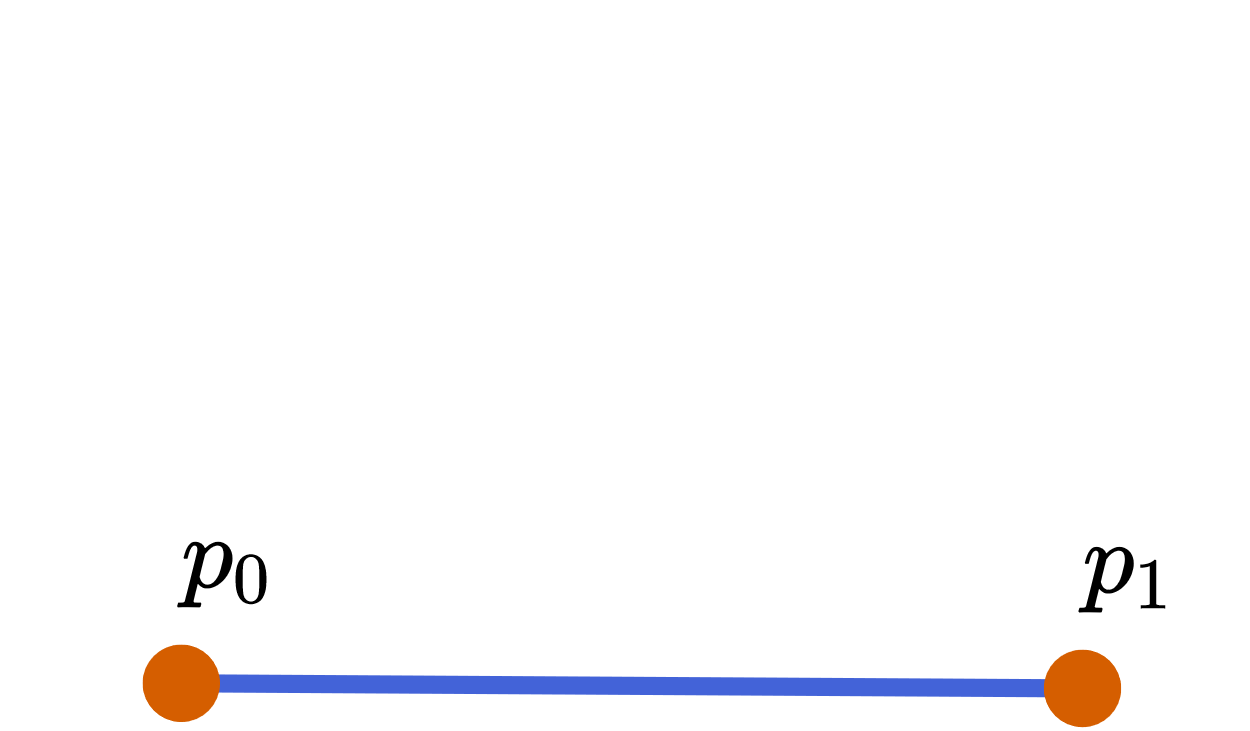
\includegraphics[width = \groupimagewidth]{images/bezier-curve-1}}
        \qquad
        \subfloat[$n=2$]{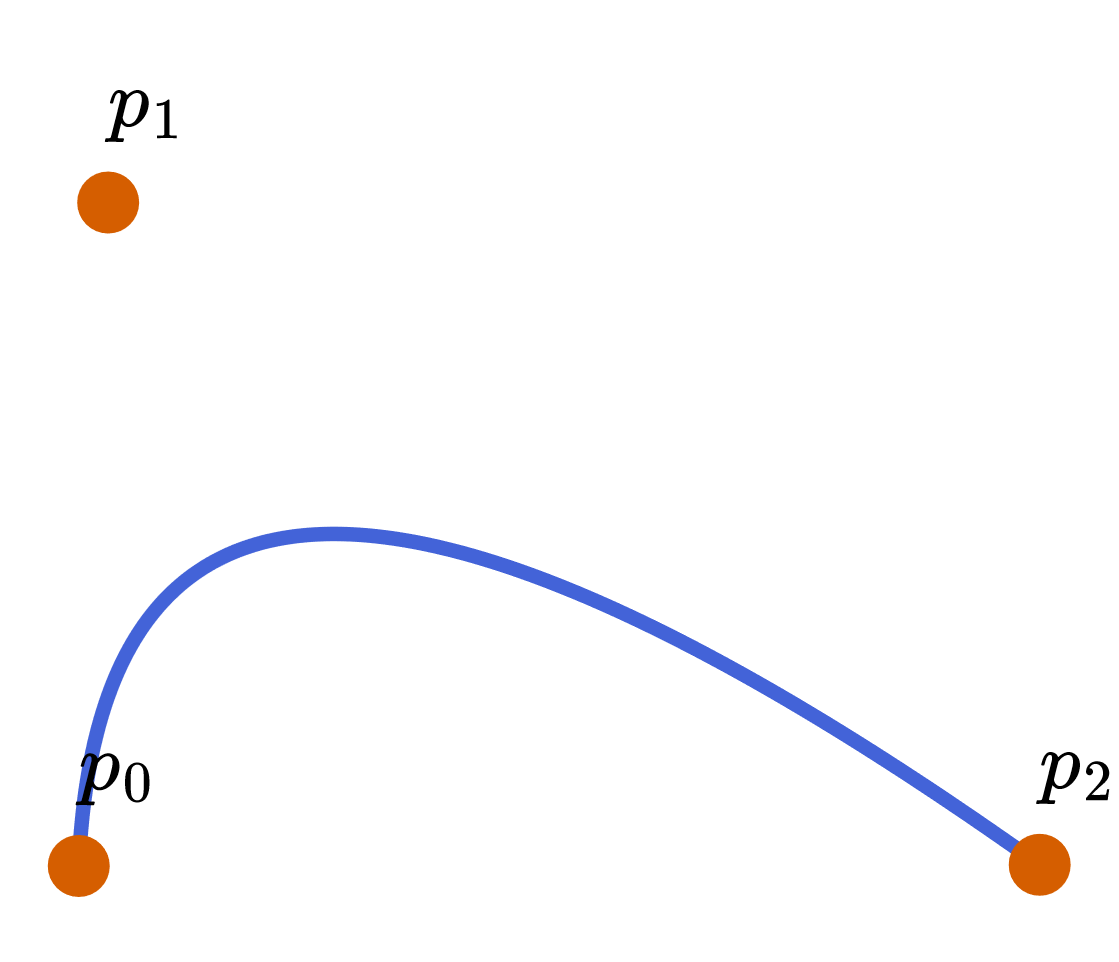
\includegraphics[width = \groupimagewidth]{images/bezier-curve-2}} \\
        \subfloat[$n=3$]{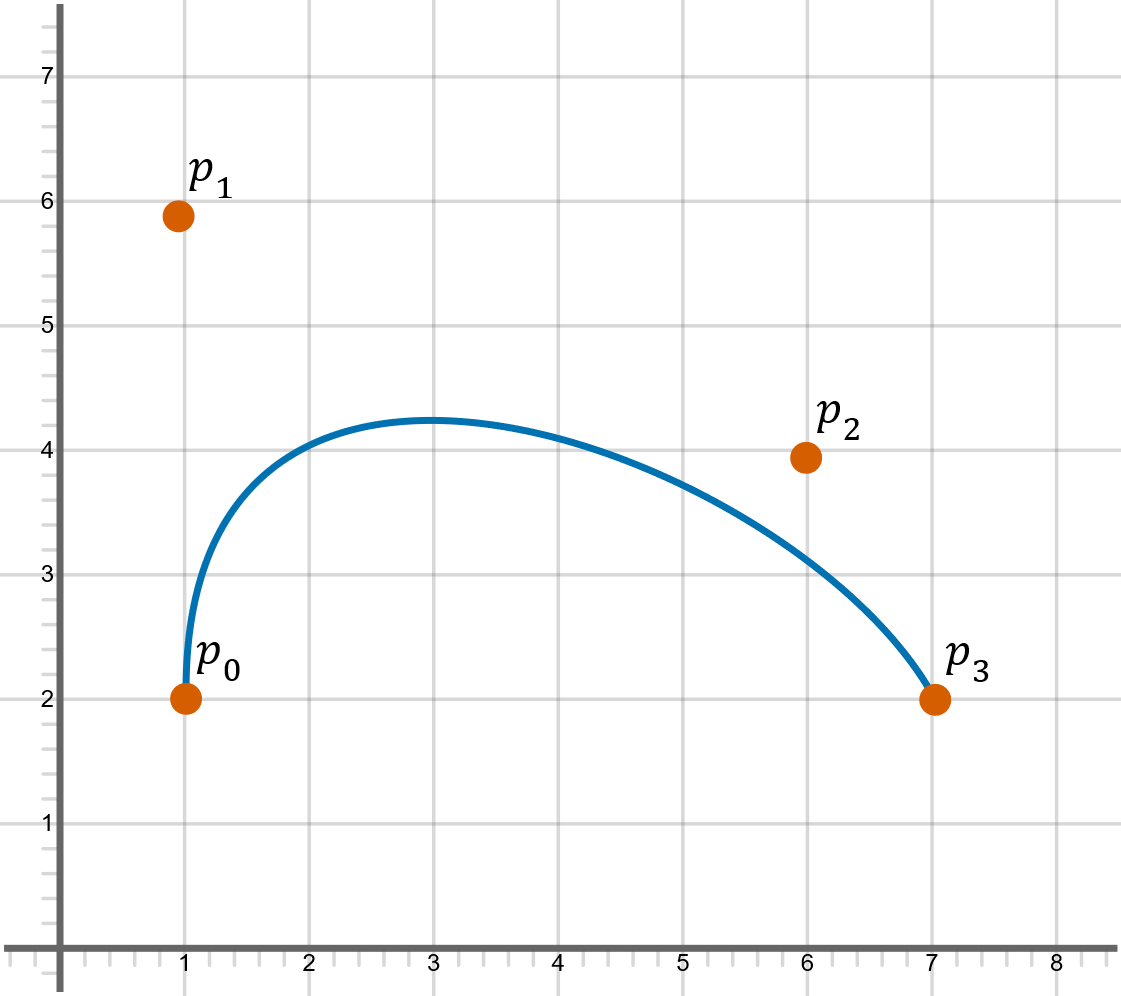
\includegraphics[width = \groupimagewidth]{images/bezier-curve-3}}
        \qquad
        \subfloat[$n=4$]{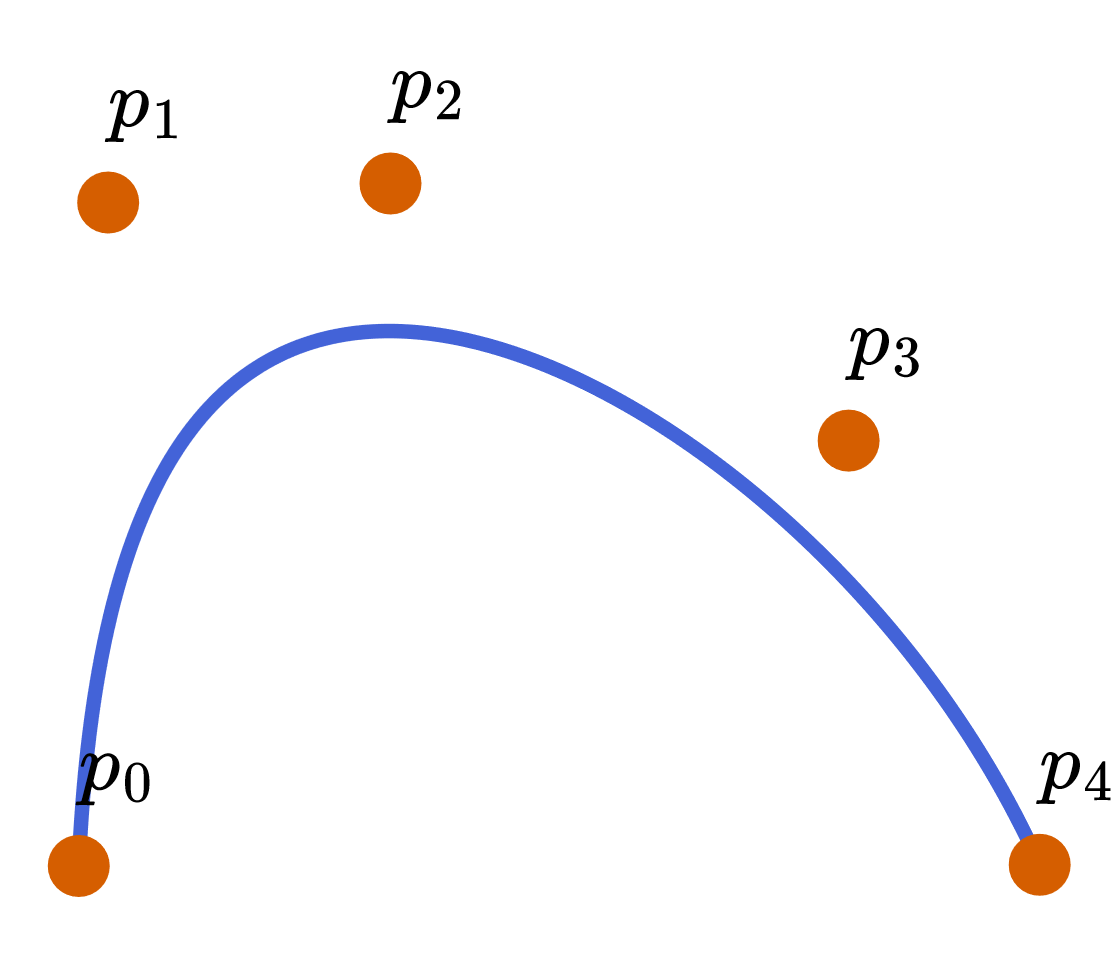
\includegraphics[width = \groupimagewidth]{images/bezier-curve-4}}
        \caption{Bézierjeve krivulje s pripadajočimi kontrolnimi poligoni za stopnje $n=1,2,3,4$.}
        \label{fig:bezierjeva-krivulja}
    \end{figure}

    Zapišimo sedaj nekaj osnovnih lastnosti Bézierjevih krivulj.
    \begin{izrek}{Bézierjeva krivulja $\mathbf{B}$ s kontrolnimi točkami $\p_i$, $i=0,1\ldots,n$, ima sledeče lastnosti.}
        \label{izrek:lastnosti-bezierjevih-krivulj}
        \begin{enumerate}
            \item Interpolira končni točki, tj.\ velja $\mathbf{B}(0)=\p_0$ in $\mathbf{B}(1)=\p_n$.
            \item Je afino invariantna, tj.\ za poljubno afino transformacijo $A$ velja \[A \left(\bernsteinsump{i}{n}\right) =\bernsteinsumtritri{i}{n}{A(\p_i)}.\]
            \item Leži znotraj konveksne ovojnice svojih kontrolnih točk.
        \end{enumerate}
    \end{izrek}
    \noindent Dokazi lastnosti so enostavni, zato jih izpustimo.
    Preden si lastnosti ogledamo na slikah povejmo, zakaj so pomembne za CAGD sisteme.
    Interpolacija končnih točk uporabniku omogoča kontrolo nad tem, kje se bo krivulja začela in kje zaključila.
    Zaradi afine invariance lahko uporabnikove transformacije krivulje v ozadju CAGD sistema prevedemo v transformacije kontrolnih točk.
    Tretja lastnost pa uporabniku s kontrolnimi točkami omogoča upravljanje krivulje, kjer je krivulja zmerom v bližini svojih kontrolnih točk.
    Lastnosti si sedaj oglejmo na slikah.
    Interpolacijo končnih točk je bilo moč videti že na sliki~\ref{fig:bezierjeva-krivulja}.
    Posledice afine invariance si lahko ogledamo na sliki~\ref{fig:bezier-affine-transform}.
    Na sliki~\ref{fig:bezier-convex-hull} pa si lahko ogledamo konveksni ovojnici kontrolnih točk dveh Bézierjevih krivulj.
    Vidimo, da krivulji ležita znotraj njih.
    \begin{figure}[ht!]
        \captionsetup[subfigure]{labelformat=empty}
        \centering
        \subfloat[začetna krivulja]{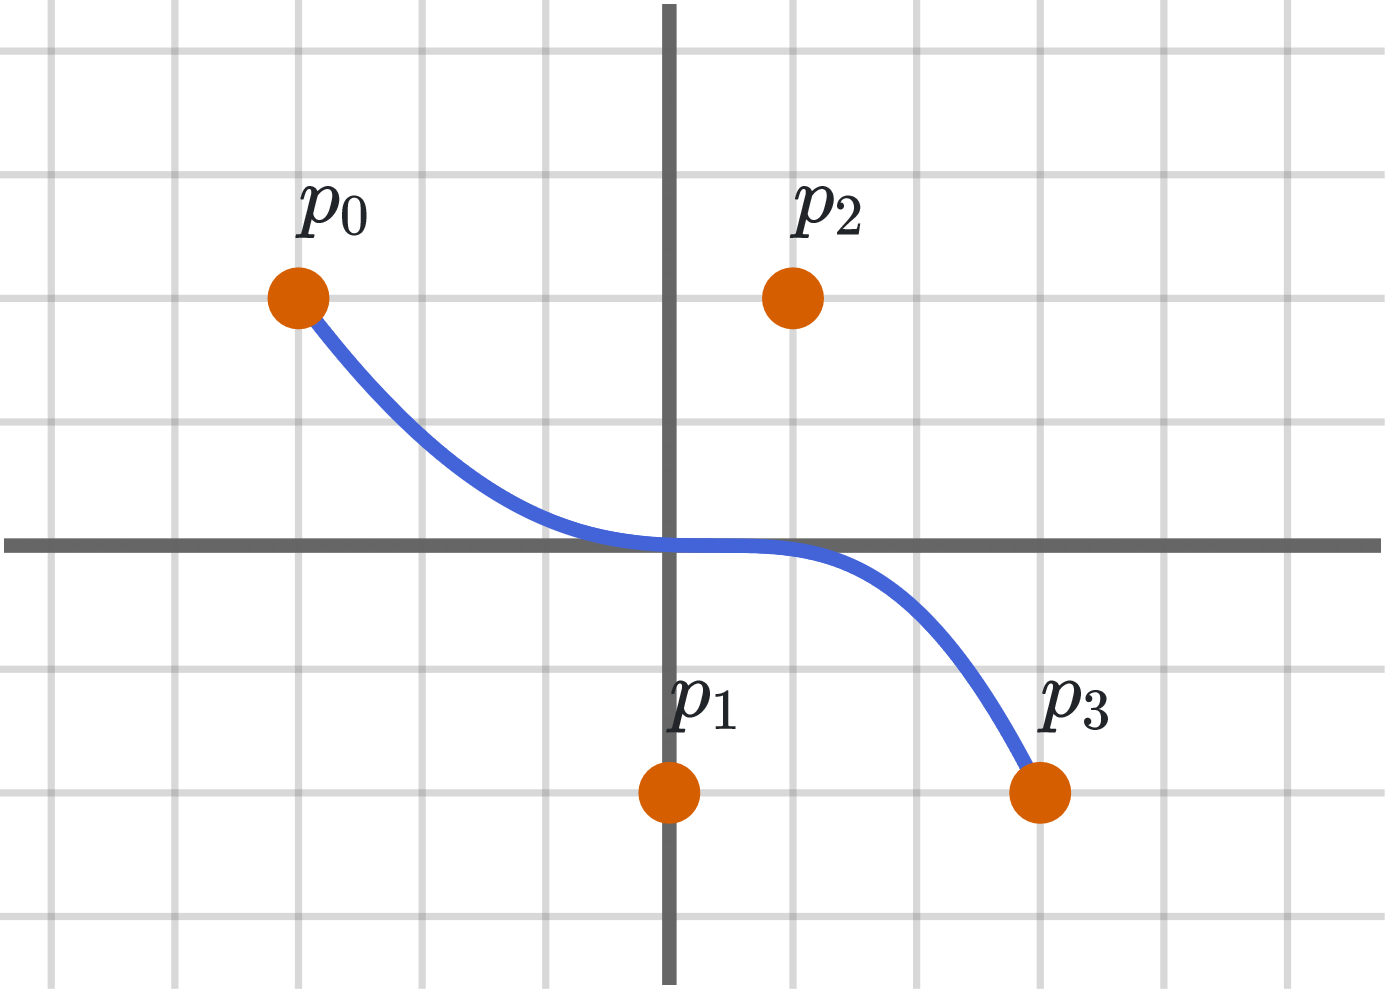
\includegraphics[width = \groupimagewidth]{images/afine-transform-start}}
        \qquad
        \subfloat[povečanje]{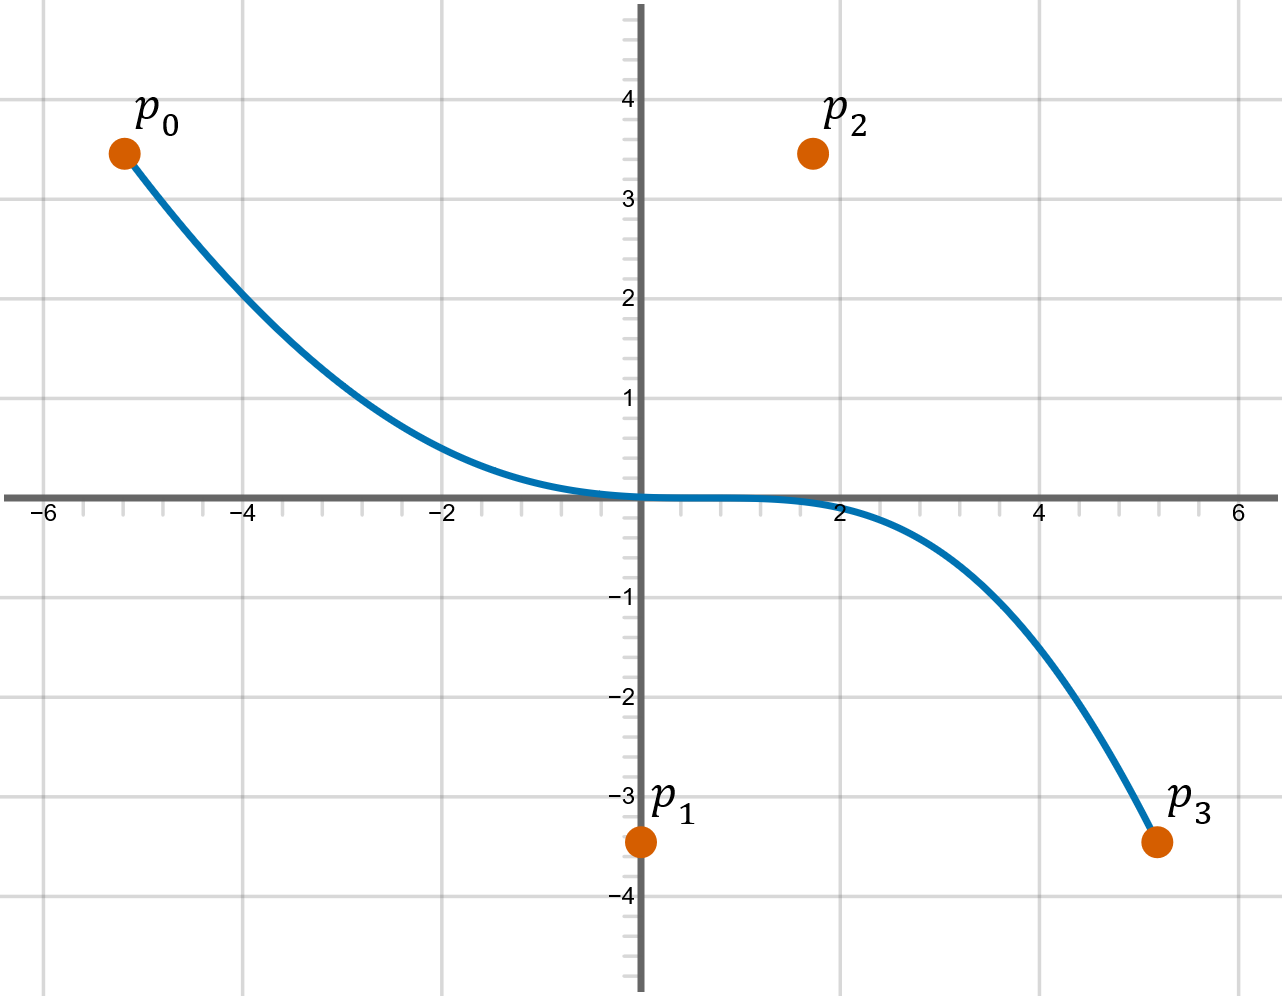
\includegraphics[width = \groupimagewidth]{images/afine-transform-bigger}} \\
        \subfloat[zrcaljenje čez $x$ os]{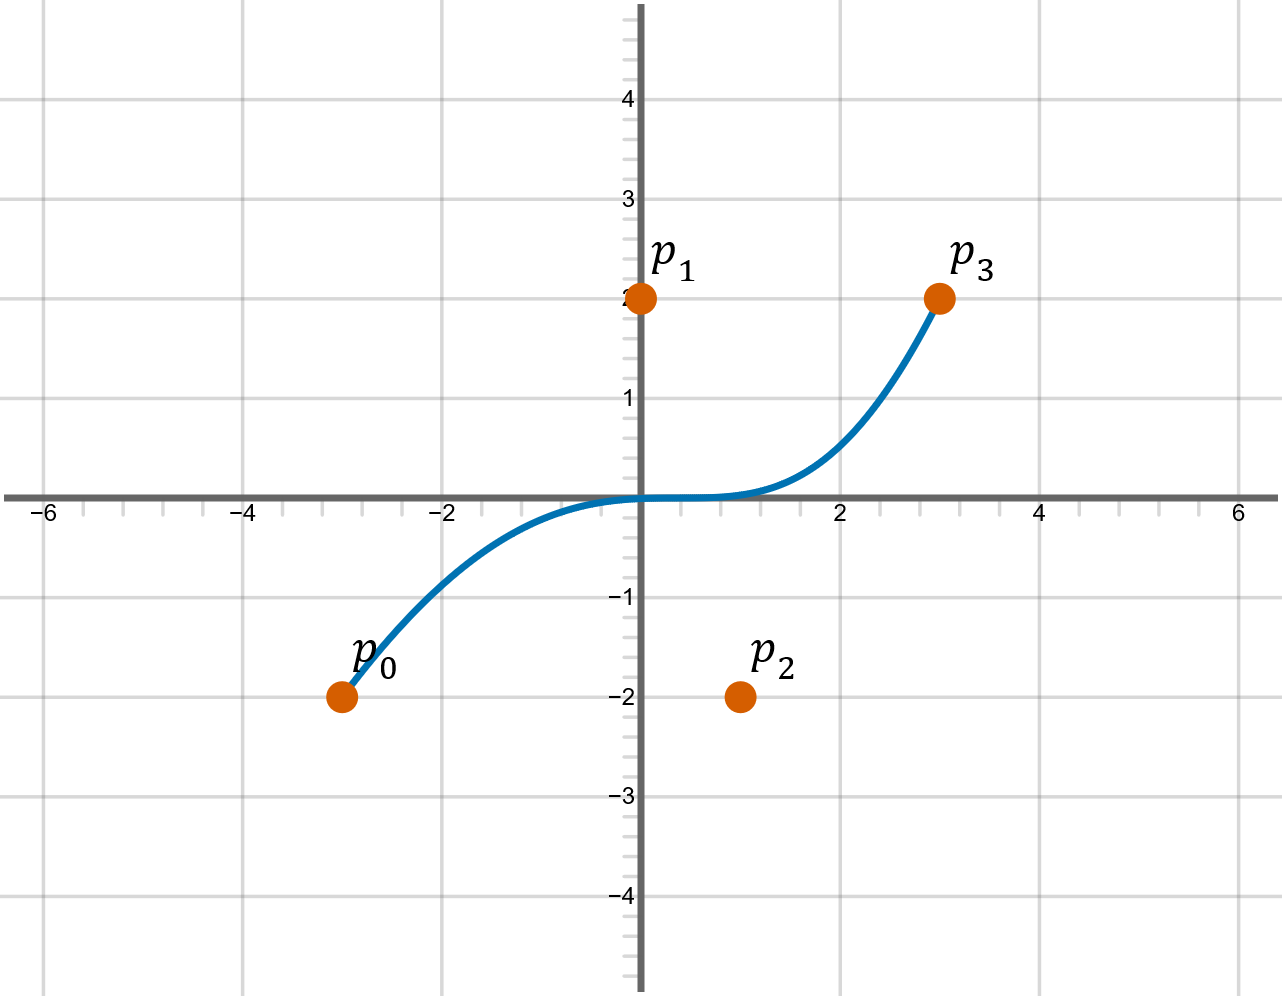
\includegraphics[width = \groupimagewidth]{images/afine-transform-flip}}
        \qquad
        \subfloat[rotiranje za $\frac{\pi}{2}$]{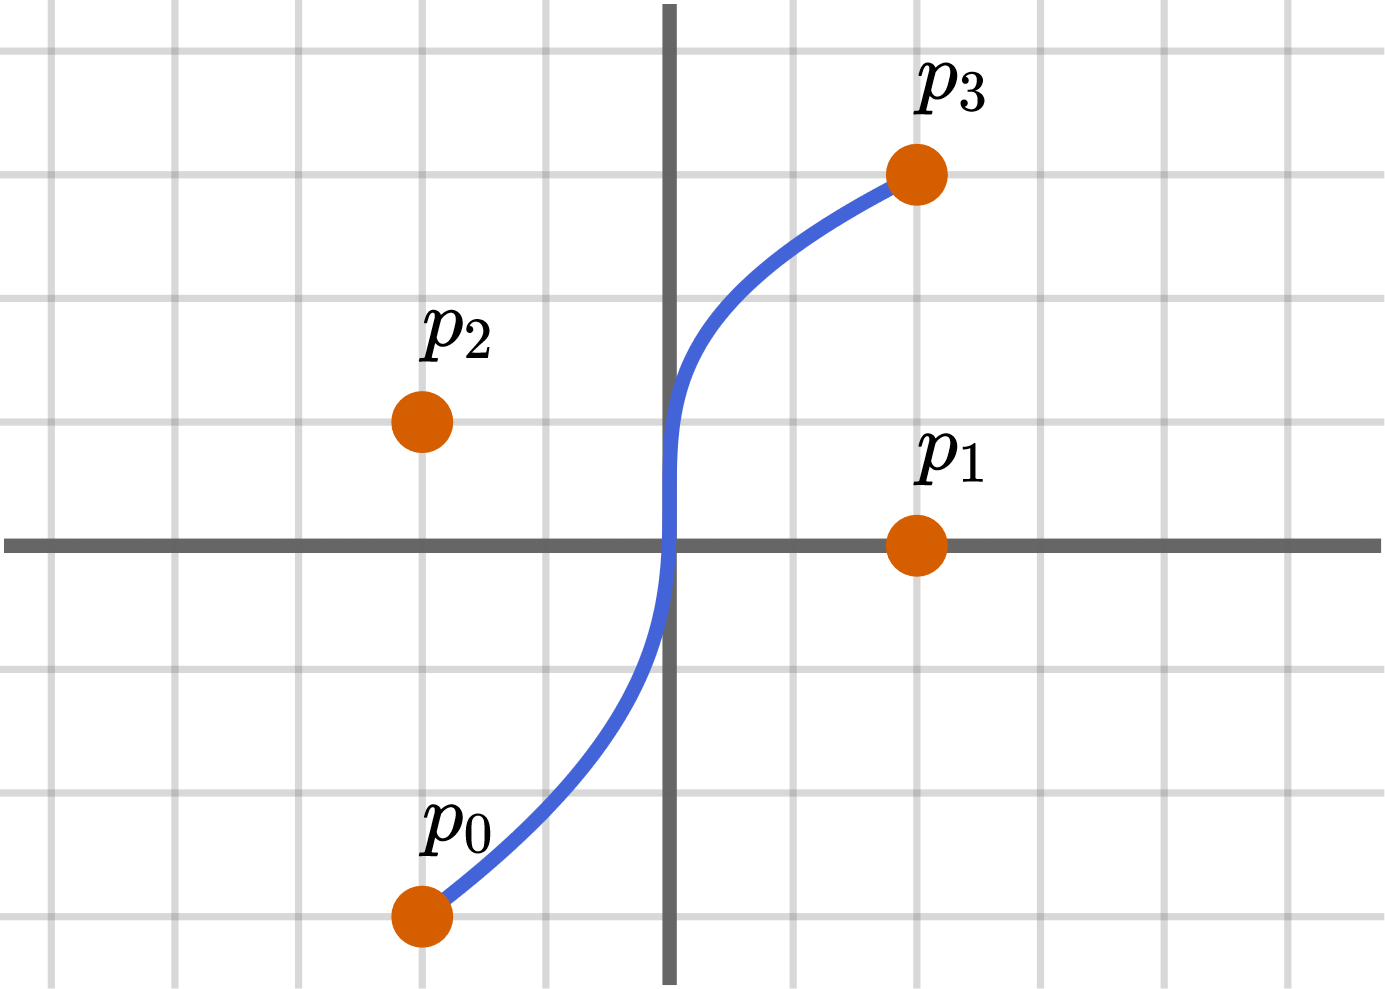
\includegraphics[width = \groupimagewidth]{images/afine-transform-rotate}}
        \caption{Afine transformacije Bézierjeve krivulje.}
        \label{fig:bezier-affine-transform}
    \end{figure}
    \begin{figure}[ht!]
        \captionsetup[subfigure]{labelformat=empty}
        \centering
        \subfloat[]{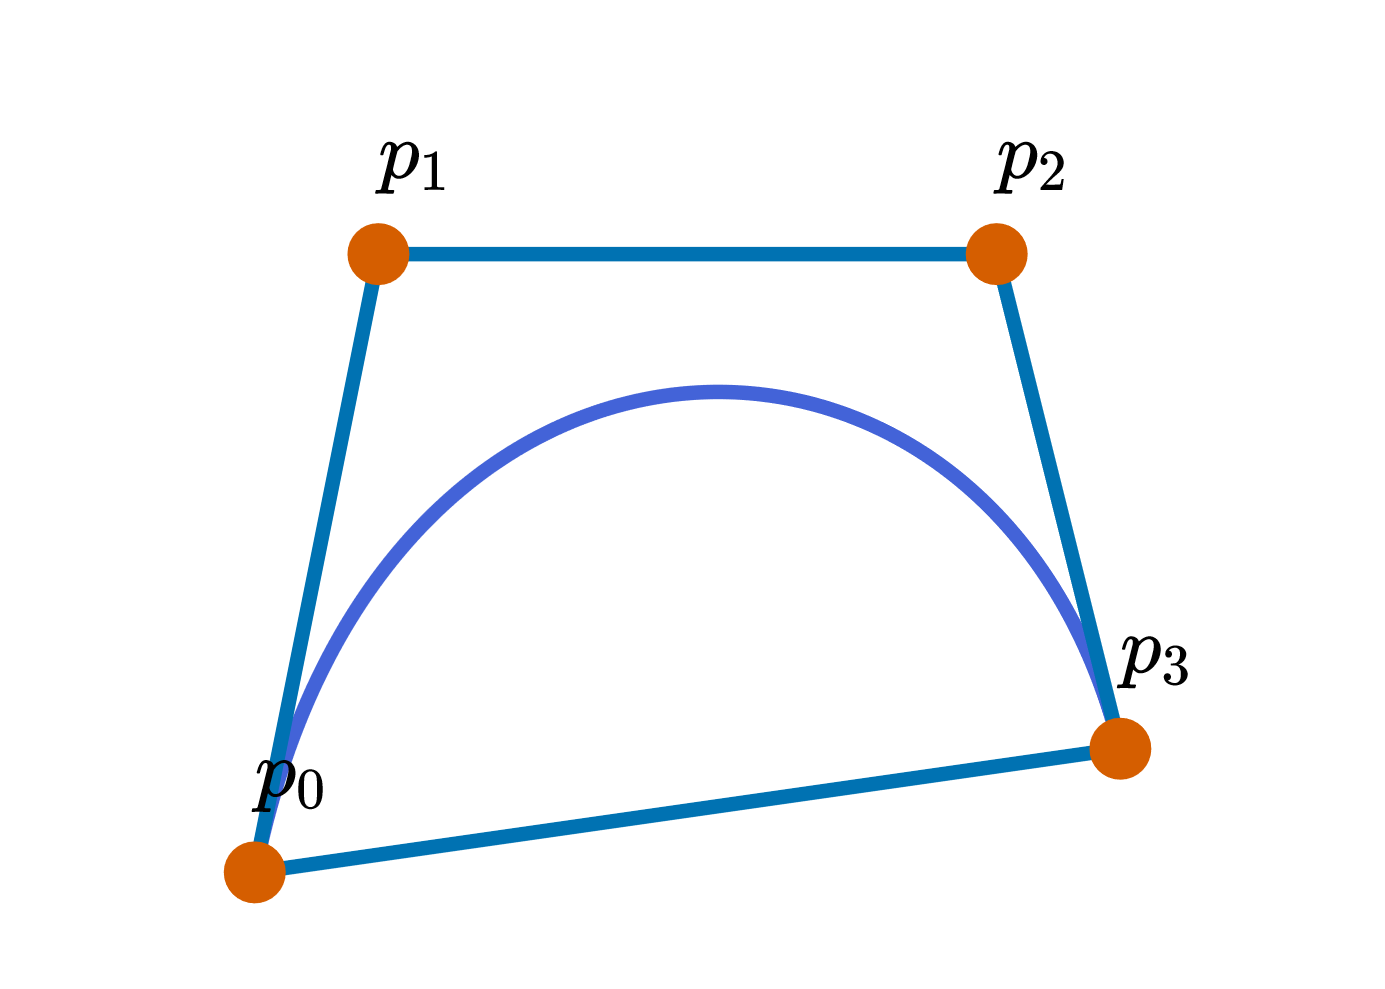
\includegraphics[width = \groupimagewidth]{images/bezier-curve-convex-hull-1}}
        \qquad
        \subfloat[]{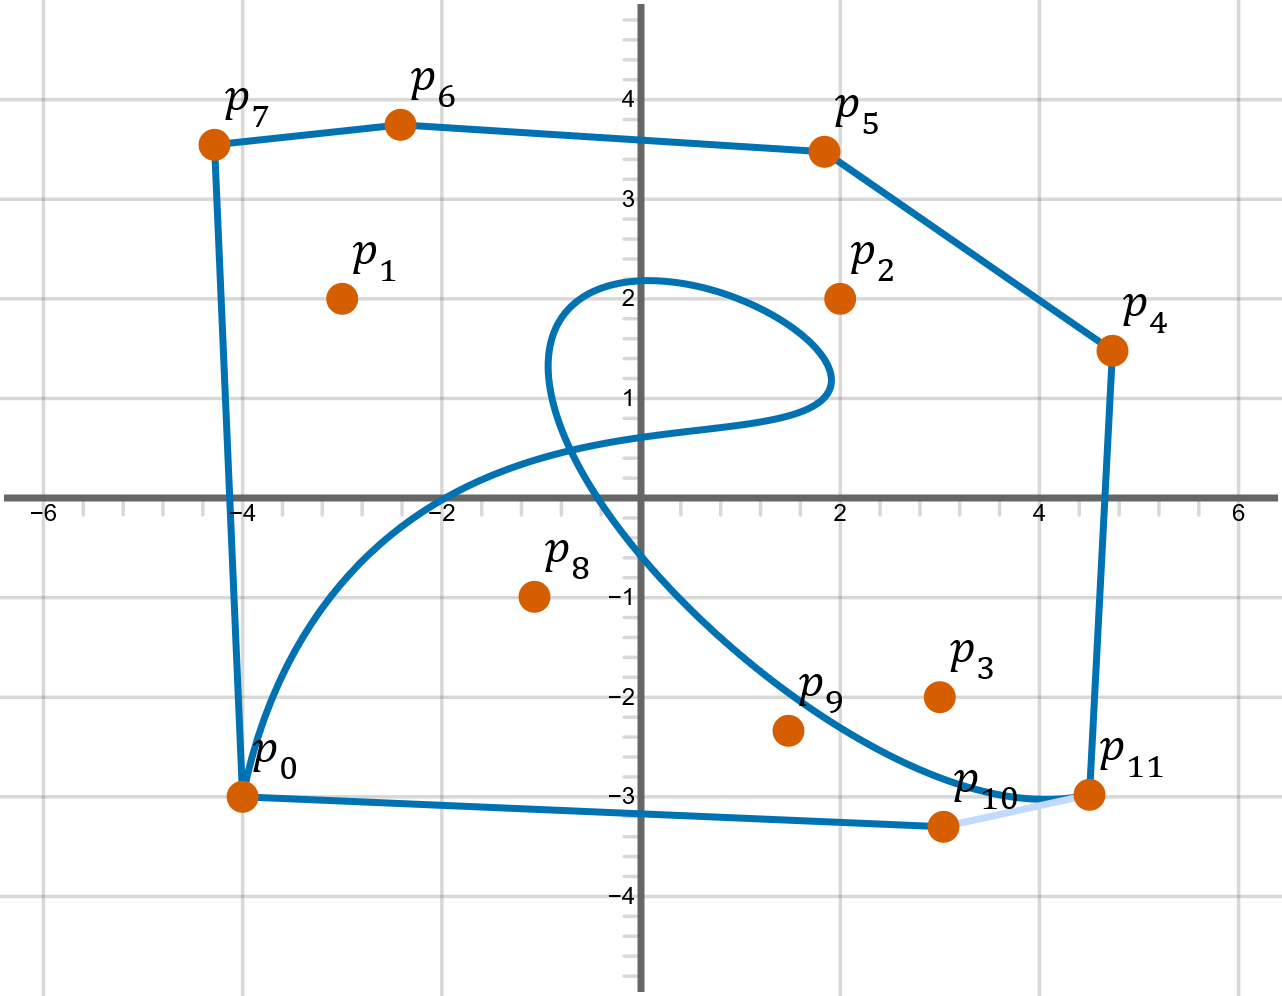
\includegraphics[width = \groupimagewidth]{images/bezier-curve-convex-hull-2}}
        \caption{Konveksni ovojnici kontrolnih točk Bézierjevih krivulj.}
        \label{fig:bezier-convex-hull}
    \end{figure}
%    Izrek~\ref{izrek:lastnosti-bezierjevih-krivulj} sedaj tudi dokažimo.
%    \begin{dokaz}
%        \noindent Lastnost (1) dokažemo s pomočjo izreka~\ref{izrek:bernsteinovi_lastnosti}.
%        Iz njega sledi
%        \[ \bigbbod{n}{0}=\sum_{i=0}^{n}\p_{i}B_i^n(t)(0) = \sum_{i=0}^{n}\p_{i}\delta_{0,i} = \p_0.\]%,\ \text{in} \ \bigbbod{n}{1}=\sum_{i=0}^{n}\p_{i}B_i^n(t)(1) = \sum_{i=0}^{n}\p_{i}\delta_{n,i} = \p_n\]
%        Podobno lahko naredimo tudi za $\bigbbod{n}{1}.$
%        Dokažimo sedaj lastnost (2).
%        Naj bo $\varphi$ afina preslikava.
%        Zanjo torej velja $\varphi(x) = A\mathbf{x} + \mathbf{b}$.
%        Potem za afino transformacijo Bézierjeve krivulje velja
%        \begin{align*}
%            \varphi\left(\sum_{i=0}^{n}\p_{i}B_i^n(t)(t)\right) &= A\left(\sum_{i=0}^{n}\p_{i}B_i^n(t)(t)\right) + \mathbf{b} &&=  \sum_{i=0}^{n}A\p_{i}B_i^n(t)(t) + \mathbf{b}  \\
%            &= \sum_{i=0}^{n}A\p_{i}B_i^n(t)(t) + \sum_{i=0}^{n}\mathbf{b}B_i^n(t)(t) &&= \sum_{i=0}^{n}(A\p_{i}+\mathbf{b})B_i^n(t)(t) \\
%            &= \bernsteinsumtritri{i}{n}{\varphi(\p_i).}
%        \end{align*}
%        Kar smo tudi želeli dokazati.
%        Za lastnost (3) posežemo po definiciji konveksne ovojnice.
%        Konveksna ovojnica kontrolnih točk Bézierjeve krivulje je množica vseh konveksnih kombinacij teh točk, tj.\ $\sum_{i=0}^{n}\lambda_i\p_{i}$, kjer so $\lambda_i$ nenegativna realna števila za katere velja $\lambda_0 + \lambda_1 + \dots + \lambda_n = 1$.
%        Ker so Bernsteinovi polinomi razčlenitev enote in nenegativni na intervalu $[0,1]$, lahko zapišemo $\lambda_i=B_i^n(t)$.
%    \end{dokaz}

    \subsection{De Casteljaujev algoritem}
    Stabilnost metod je v CAD in CAGD sistemih bistvene narave.
    Direktno računanje vrednosti Bernsteinovih polinomov preko izrazov iz definicije~\ref{def:bernstein} pa ni stabilno~\cite{stability}.
    Da lahko točke Bézierjevih krivulj računamo stabilno, potrebujemo sledeč izrek.
    \begin{izrek}
        \label{izrek:decastelaju-rekurzija}
        Označimo z $\mathbf{B}_{[\p_0,\p_1,\dots,\p_n]}$ Bézierjevo krivuljo s kontrolnimi točkami \\
        $\p_0,\p_1,\dots,\p_n$.
        Potem za poljubno realno število $t$ in naravno število $n$ velja rekurzivna zveza \[\bigbbt_{[\p_0,\p_1,\dots,\p_n]} = (1-t)\bigbbt_{[\p_0,\p_1,\dots,\p_{n-1}]} +t\bigbbt_{[\p_1,\p_2,\dots,\p_n]}.\]
    \end{izrek}
    \noindent Izrek s pomočjo indukcije tudi dokažimo.
    \begin{dokaz}
        Za $n=1$ zveza drži, saj je  \[\bigbbt_{[\p_0,\p_1]} = (1-t)\p_2 +t\p_1 = (1-t)\bigbbt_{[\p_0]} +t\bigbbt_{[\p_1]}.\]
        Indukcijski korak pa dokažemo tako, da v desni del rekurzivne zveze iz izreka vstavimo parametrizaciji Bézierjevih krivulj in dobimo
        \[ (1-t) \bigbbt_{[\p_0,\p_1,\dots,\p_{n-1}]}+t\bigbbt_{[\p_1,\p_2,\dots,\p_n]} = (1-t)\bernsteinsump{i}{n-1}+t\sum_{i=0}^{n-1} \p_{i+1}B_i^{n-1}(t).\]
        Nato zamaknemo indeks desne vsote in skupne točke postavimo pod eno vsoto.
        Od tod sledi
        \begin{align*}
            &(1-t)\bernsteinsump{i}{n-1}+ t\sum_{i=1}^{n} \p_{i}B_{i-1}^{n-1}(t) \\
            %  &= \p_0(1-t)B_{0}^{n-1}(t) + \sum_{i=1}^{n-1}\p_{i}(1-t)B_i^{n-1}(t) +  \sum_{i=1}^{n-1} \p_{i}tB_{i-1}^{n-1}(t) + \p_n B_{n-1}^{n-1}(t) \\
            &= \p_0(1-t)B_{0}^{n-1}(t) + \sum_{i=1}^{n-1}\left((1-t)B_i^{n-1}(t) + tB_{i-1}^{n-1}(t)\right)\p_{i} + \p_n B_{n-1}^{n-1}(t). \\
        \end{align*}
        Uporabimo še rekurzivno zvezo Bernsteinovih baznih polinomov iz izreka~\ref{izrek:bernsteinovi_lastnosti:rekruzija}, da dobimo
        \begin{align*}
            \p_0B_{0}^{n}(t) + \sum_{i=1}^{n-1}\p_{i}B_i^n(t) + \p_n B_{n}^{n}(t) = \sum_{i=0}^{n}\p_{i}B_i^n(t).
        \end{align*}
    \end{dokaz}
    \noindent Na sliki~\ref{fig:decasteljau-2} lahko vidimo, kako lahko točke Bézierjeve krivulje $\mathbf{B}_{[\p_0,\p_1,\p_2,\p_3,\p_4]}$ računamo s pomočjo točk Bézierjevih krivulj $\mathbf{B}_{[\p_0,\p_1,\p_2,\p_3]}$ in $\mathbf{B}_{[\p_1,\p_2,\p_3,\p_4]}$.
    \begin{figure}[H]
        \captionsetup[subfigure]{labelformat=empty}
        \centering
        \subfloat[$t=0.25$]{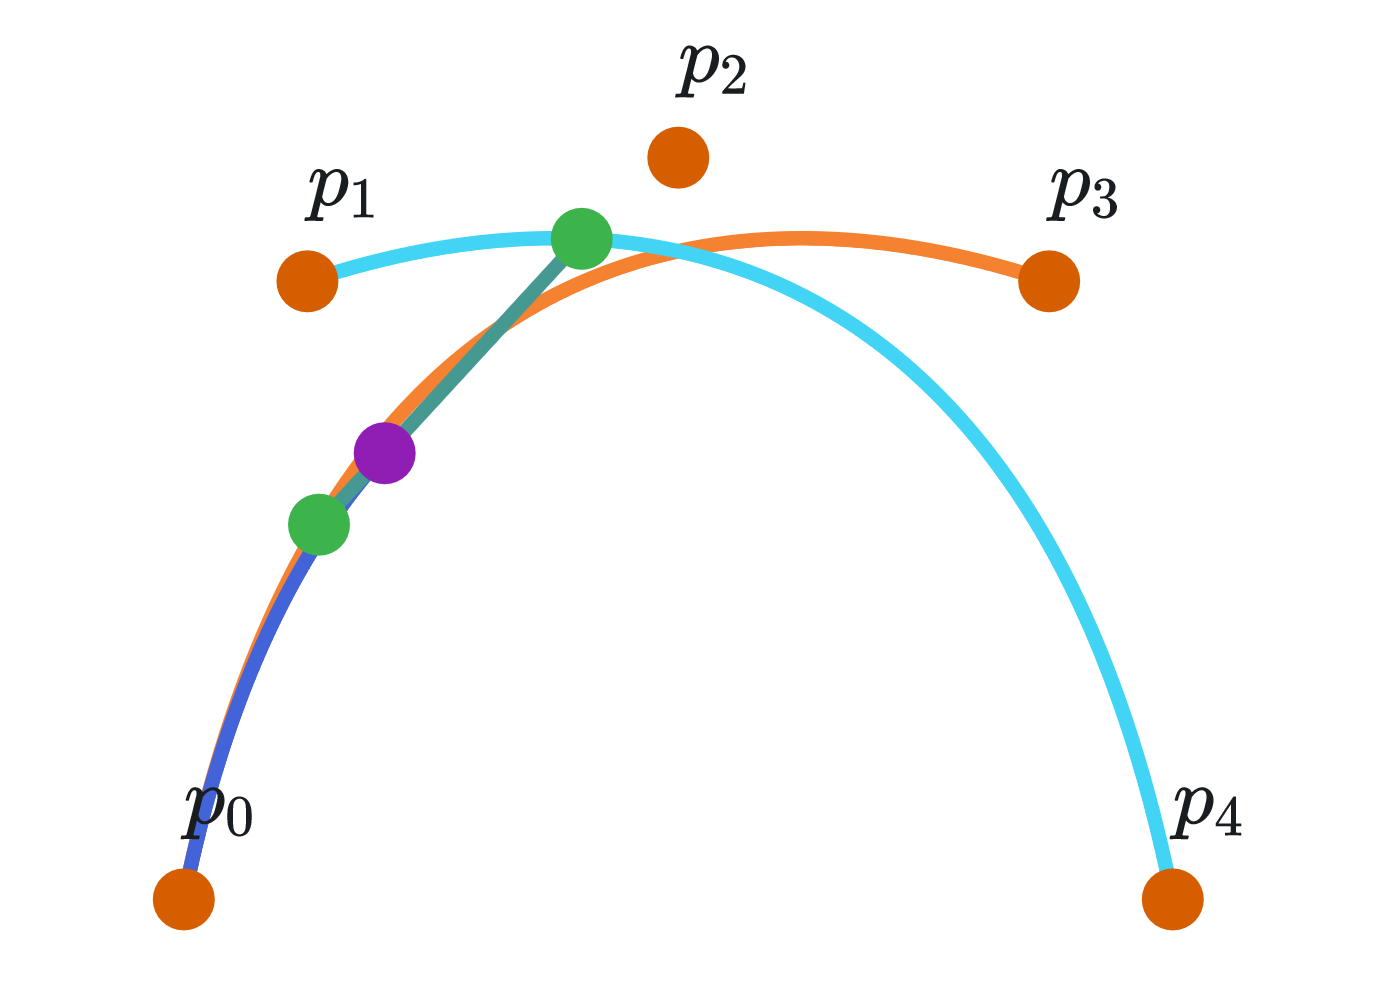
\includegraphics[width = \groupimagewidth]{images/decasteljau-2-t-025}}
        \qquad
        \subfloat[$t=0.5$]{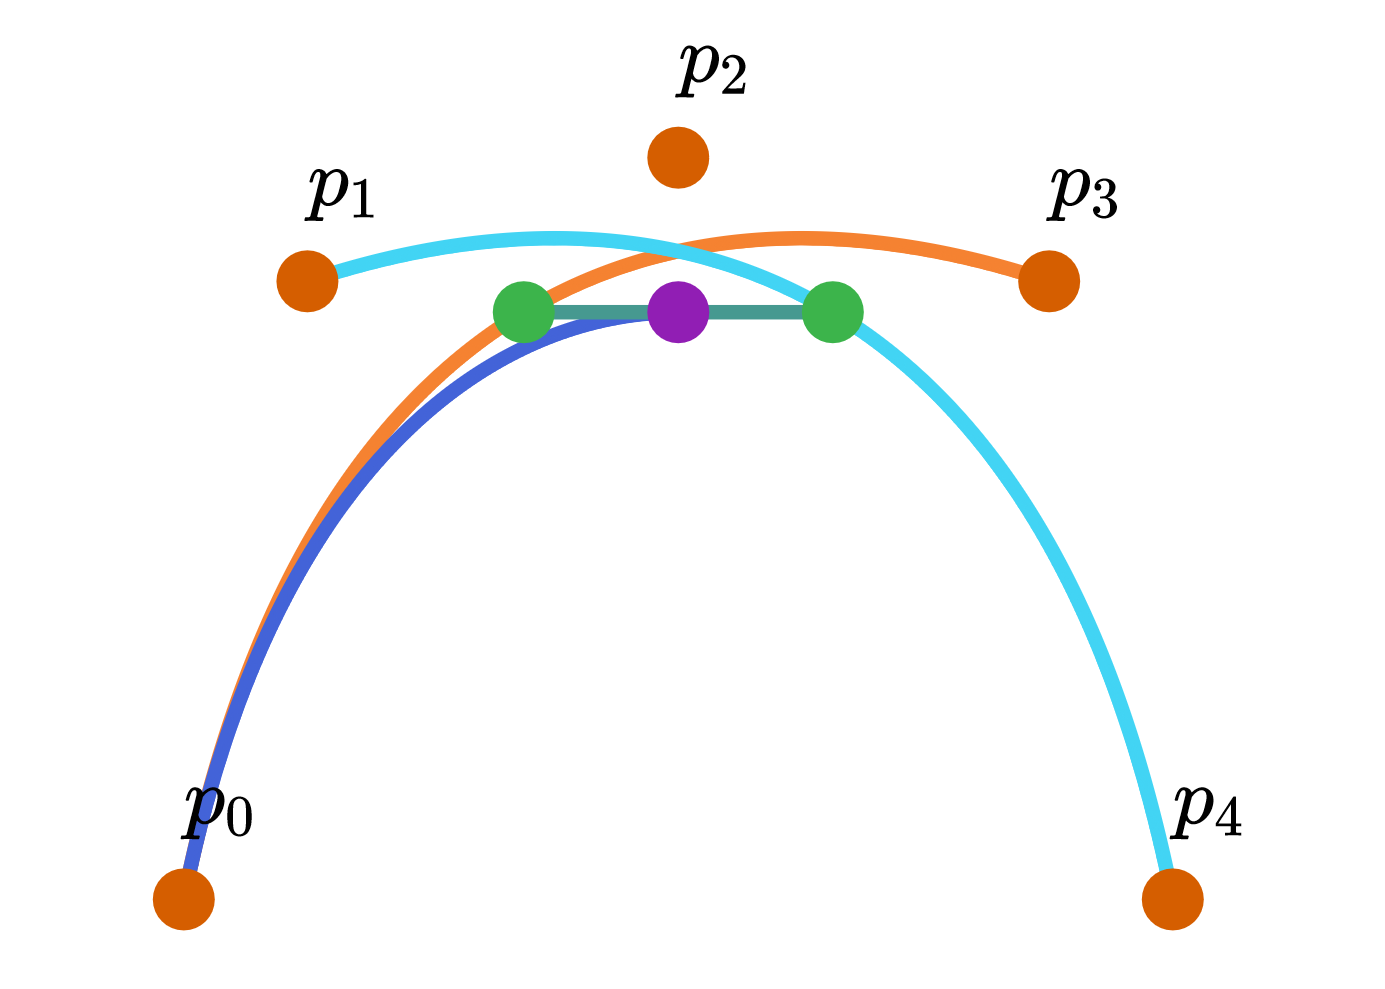
\includegraphics[width = \groupimagewidth]{images/decasteljau-2-t-05}}\\
        \subfloat[$t=0.75$]{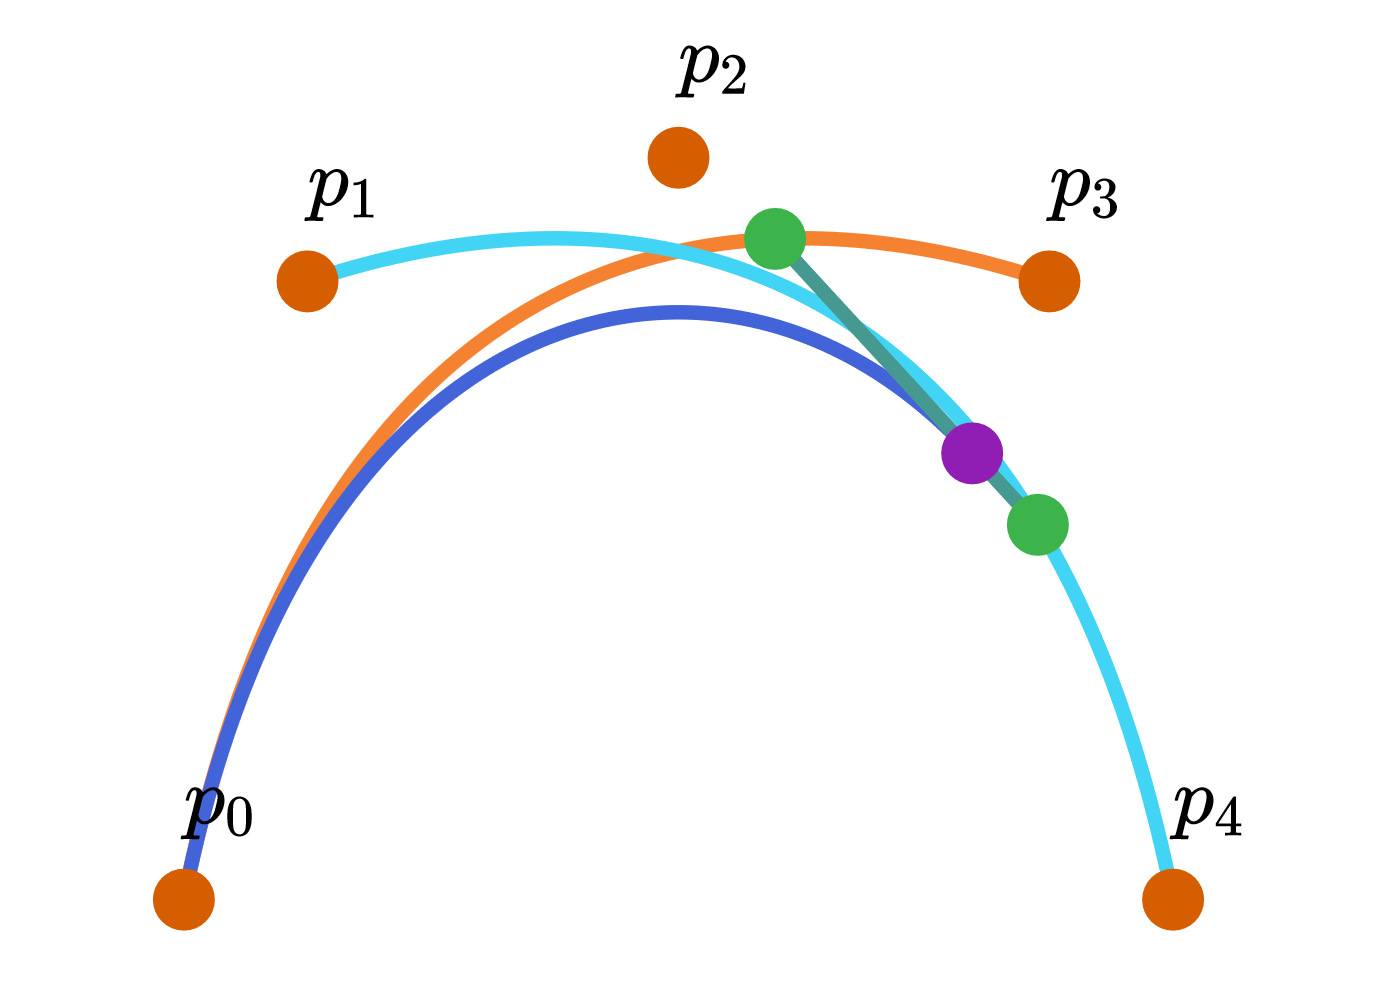
\includegraphics[width = \groupimagewidth]{images/decasteljau-2-t-075}}
        \qquad
        \subfloat[$t=1$]{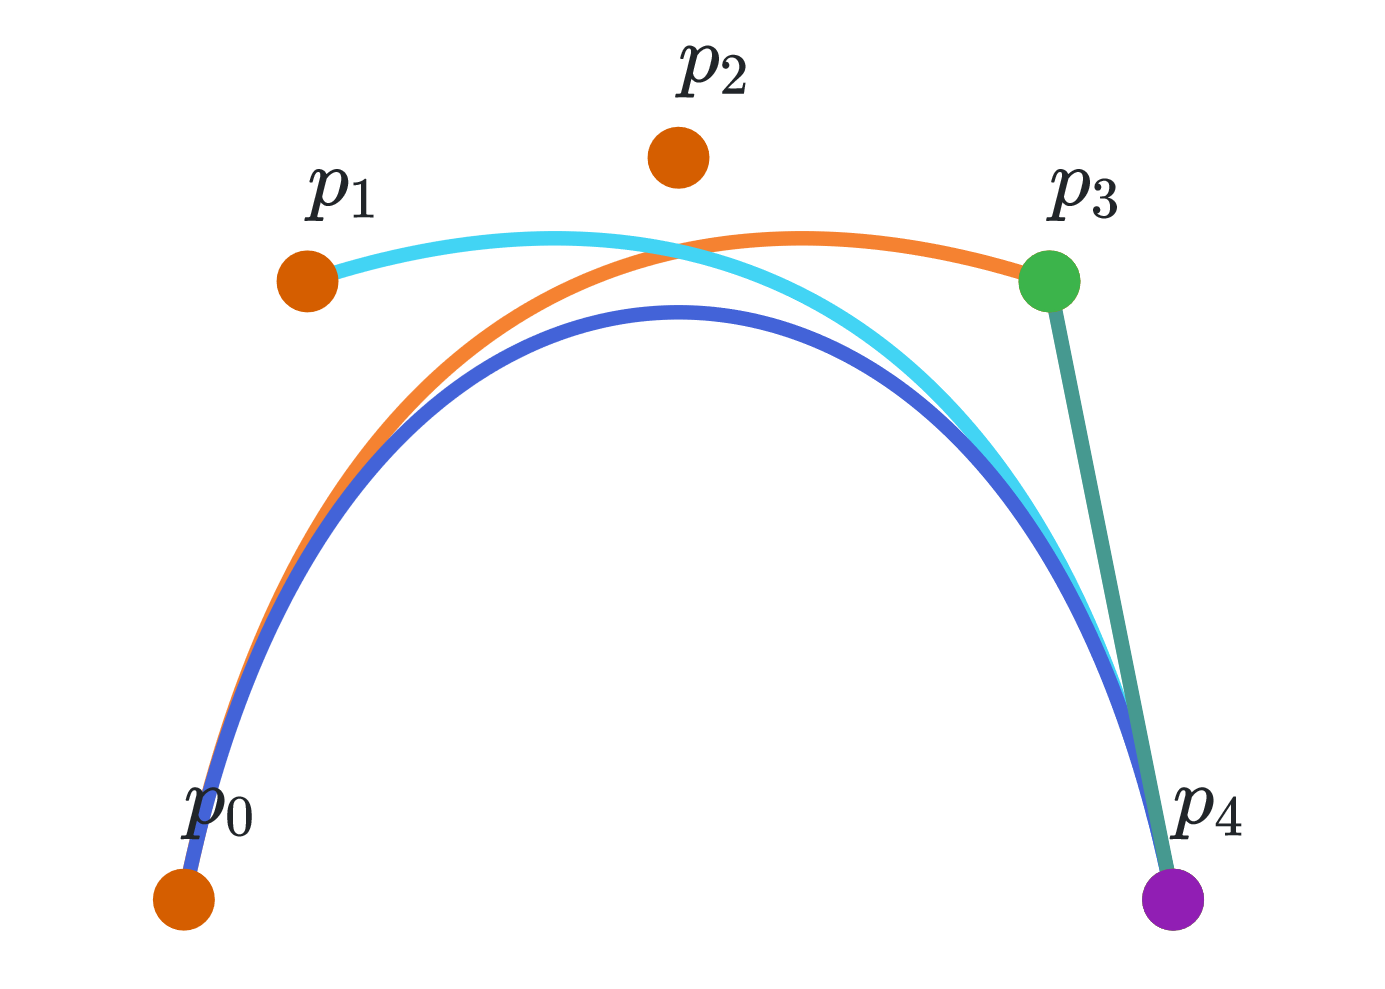
\includegraphics[width = \groupimagewidth]{images/decasteljau-2-t-1}}
        \caption{Izračun točke Bézierjeve krivulje.}
        \label{fig:decasteljau-2}
    \end{figure}

    Označimo sedaj $\p_{i}^r(t) = \bigbbt_{[\p_i,\p_{i+1},\dots,\p_{i+r}]}$.
    Velja torej $\p_{i}^0(t)=\p_i$ in  $\p_{0}^n(t)=\bigbbt_{[\p_0,\p_1,\dots,\p_n]}$.
    Iz izreka~\ref{izrek:decastelaju-rekurzija} sledi, da lahko točke Bézierjeve krivulje $\bigbbt_{[\p_0,\p_1,\dots,\p_n]}$ računamo s pomočjo \textit{de Casteljaujeve sheme}, ki jo lahko vidimo na sliki~\ref{fig:decasteljau-scheme}.
    V shemi diagonalne puščice ponazarjajo množenje točke z vrednostjo $t$, vertikalne pa z vrednostjo $1-t$.
    V vrhu puščic dobljene vrednosti seštejemo.
    \begin{figure}[H]
        \label{fig:decasteljau-scheme}
        \begin{tabular}{ c c c c c c c c c c c}
            $\p_{0}^n(t)$     &            &                   &            &               &            &          &            &                 &            &               \\
            $\uparrow$        & $\nwarrow$ &                   &            &               &            &          &            &                 &            &               \\
            $\p_{0}^{n-1}(t)$ &            & $\p_{1}^{n-1}(t)$ &            &               &            &          &            &                 &            &               \\
            $\vdots$          & $\vdots$   & $\vdots$          & $\vdots$   & $\vdots$      &            & $\vdots$ &            &                 &            &               \\
            $\uparrow$        & $\nwarrow$ & $\uparrow$        & $\nwarrow$ & $\uparrow$    & $\nwarrow$ & $\cdots$ & $\nwarrow$ &                 &            &               \\
            $\p_{0}^1(t)$     &            & $\p_{1}^1(t)$     &            & $\p_{2}^1(t)$ &            & $\cdots$ &            & $\p_{n-1}^1(t)$ &            &               \\
            $\uparrow$        & $\nwarrow$ & $\uparrow$        & $\nwarrow$ & $\uparrow$    & $\nwarrow$ & $\cdots$ & $\nwarrow$ & $\uparrow$      & $\nwarrow$     &\\
            $\p_{0}^0(t)$     &            & $\p_{1}^0(t)$     &            & $\p_{2}^0(t)$ &            & $\cdots$ &            & $\p_{n-1}^0(t)$ &            & $\p_{n}^0(t)$
        \end{tabular}
        \caption{De Casteljaujeva shema.}
    \end{figure}
    \noindent Izračun točke Bézierjeve krivulje pri poljubnem parametru $t$ lahko sedaj podamo v obliki \textit{de Casteljaujevega algoritma}~\ref{alg:decasteljau}.
    \begin{algorithm}[H]
        \caption{De Casteljaujev algoritem}
        \label{alg:decasteljau}
        \begin{algorithmic}
            \State $\p \gets \p_0,\p_1,\dots,\p_n$
            \State $t \gets t$
            \For{$i = 0,1,\dots n$}
                \State $\p_i^0(t)=\p_i$
            \EndFor
            \For{$r = 1,2,\dots n$}
                \For{$i=0,1,\dots,n-r$}
                    \State $\p_i^r(t)=(1-t)\p_i^{r-1}(t)+t\p_{i+1}^{r-1}(t)$
                \EndFor
            \EndFor
            \State \Return $\p_0^n(t)$
        \end{algorithmic}
    \end{algorithm}
    \noindent De Casteljaujev algoritem ima tudi geometrijski pomen.
    Pri stopnji $n=1$ se prevede na interpolacijo dveh točk, kar lahko vidimo na sliki~\ref{fig:dec-alg-n1}.
    Pri višjih stopnjah $n$ pa algoritem predstavlja zaporedno interpolacijo točk, saj v njem za vsak nivo $r=1,2,\ldots,n$ interpoliramo sosednje točke prejšnjega nivoja.
    Slednje lahko vidimo na slikah~\ref{fig:dec-alg-n2} in~\ref{fig:dec-alg-n3}.
    \begin{figure}[h!]
        \captionsetup[subfigure]{labelformat=empty}
        \centering
        \subfloat[$t=0.25$]{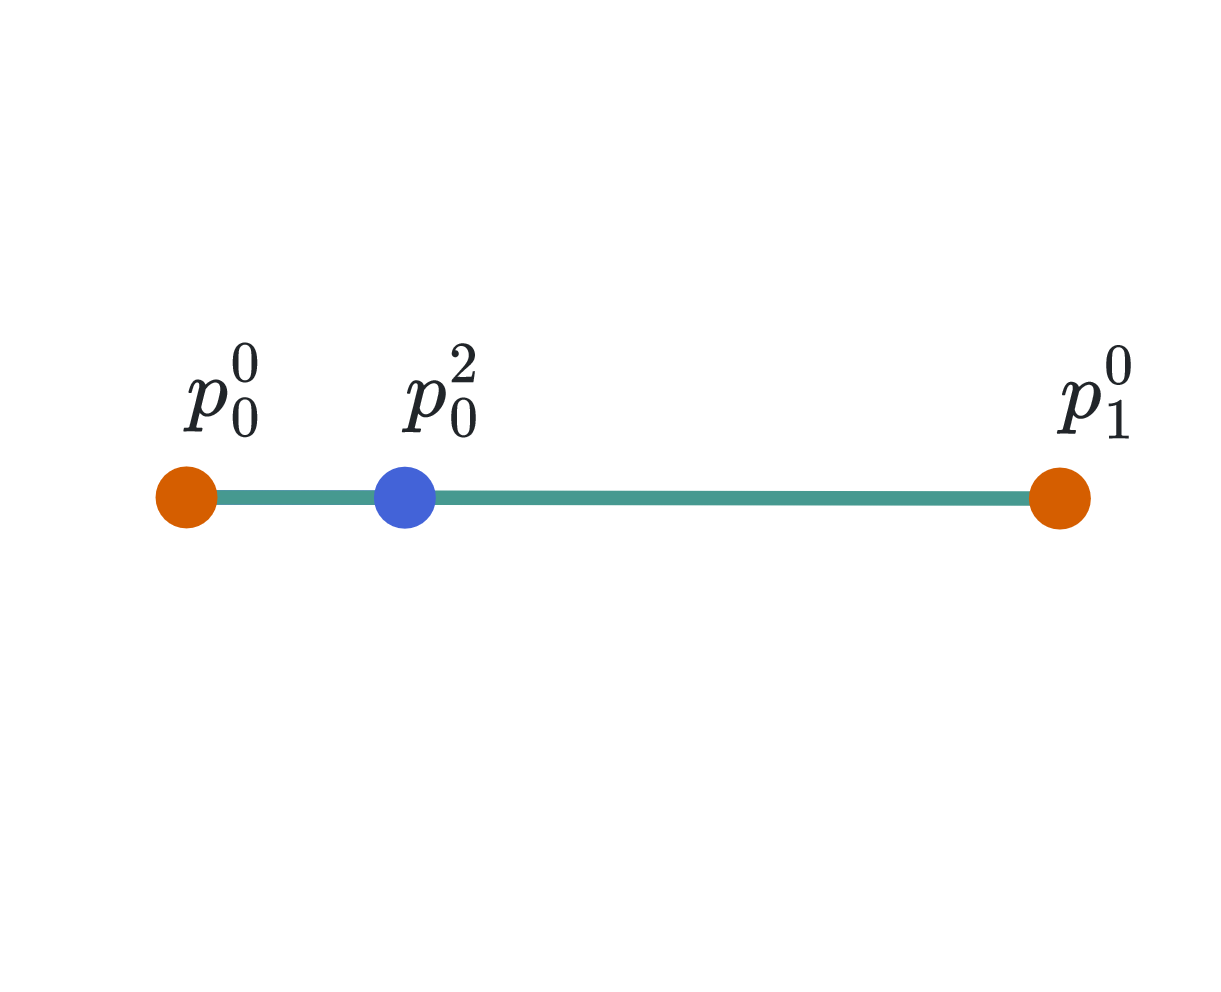
\includegraphics[width = \groupimagewidth]{images/decasteljau-n-1-t-025}}
        \qquad
        \subfloat[$t=0.5$]{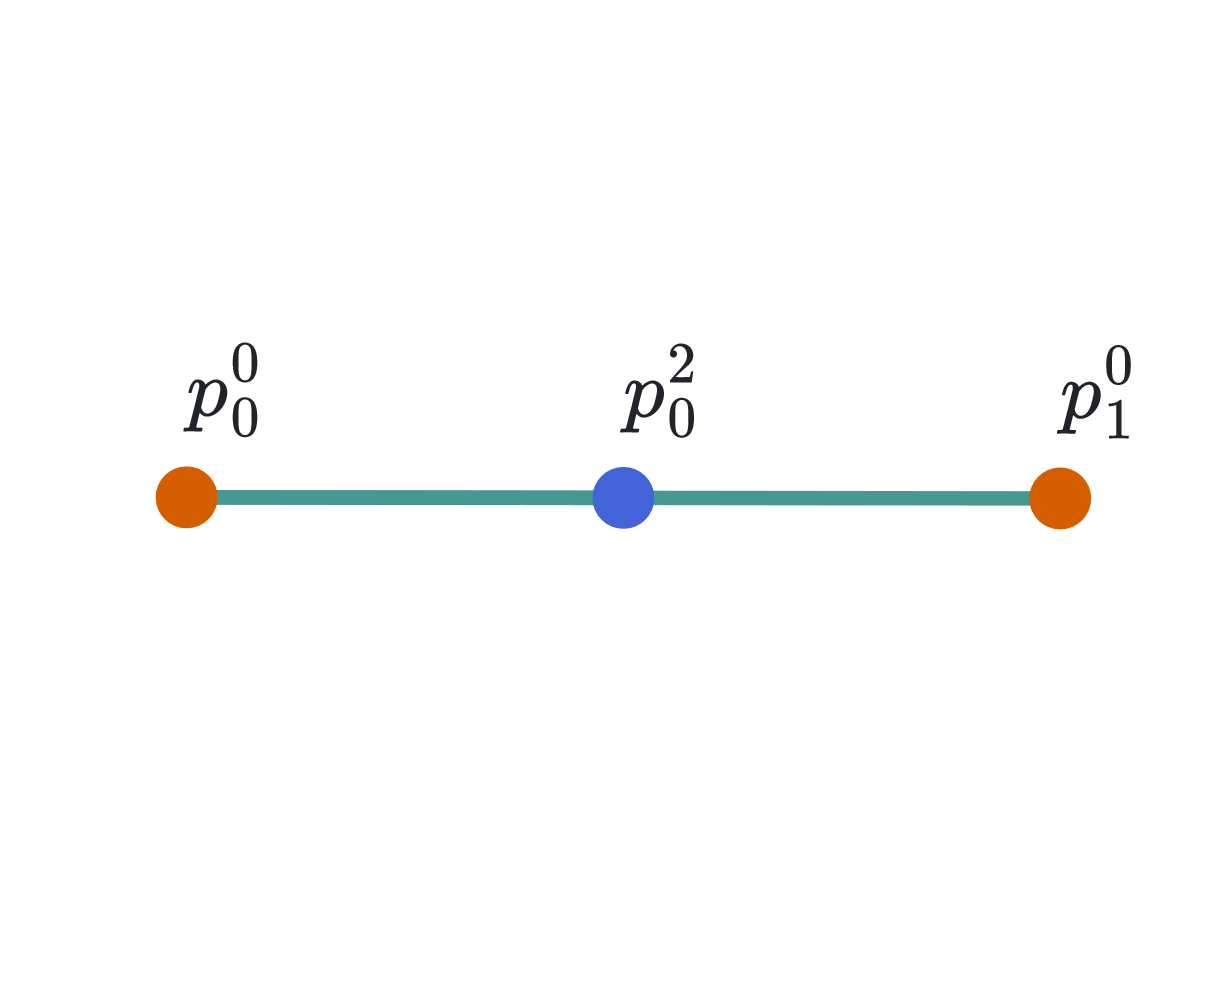
\includegraphics[width = \groupimagewidth]{images/decasteljau-n-1-t-05}}
        \\
        \subfloat[$t=0.75$]{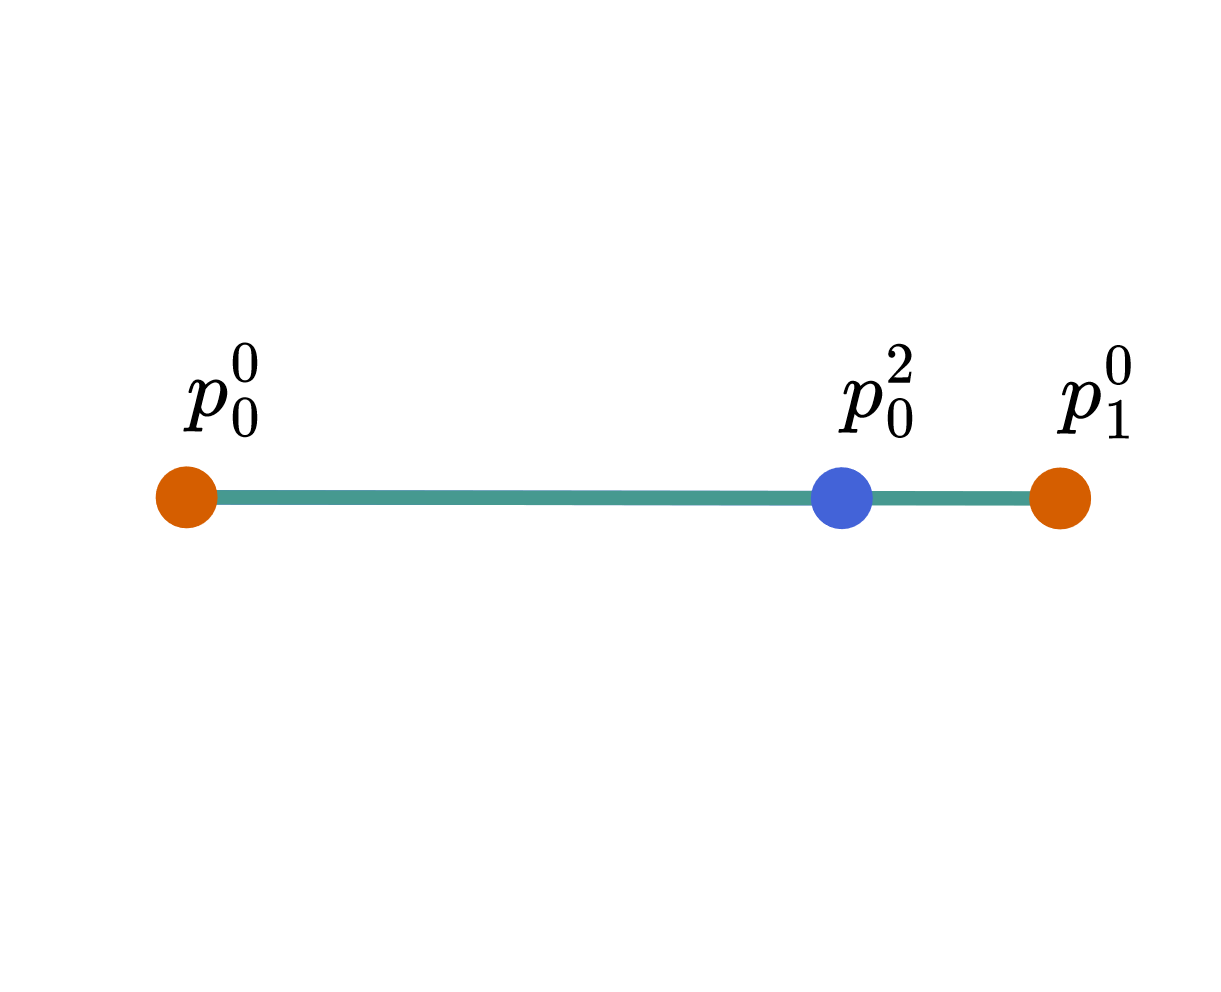
\includegraphics[width = \groupimagewidth]{images/decasteljau-n-1-t-075}}
        \qquad
        \subfloat[$t=1$]{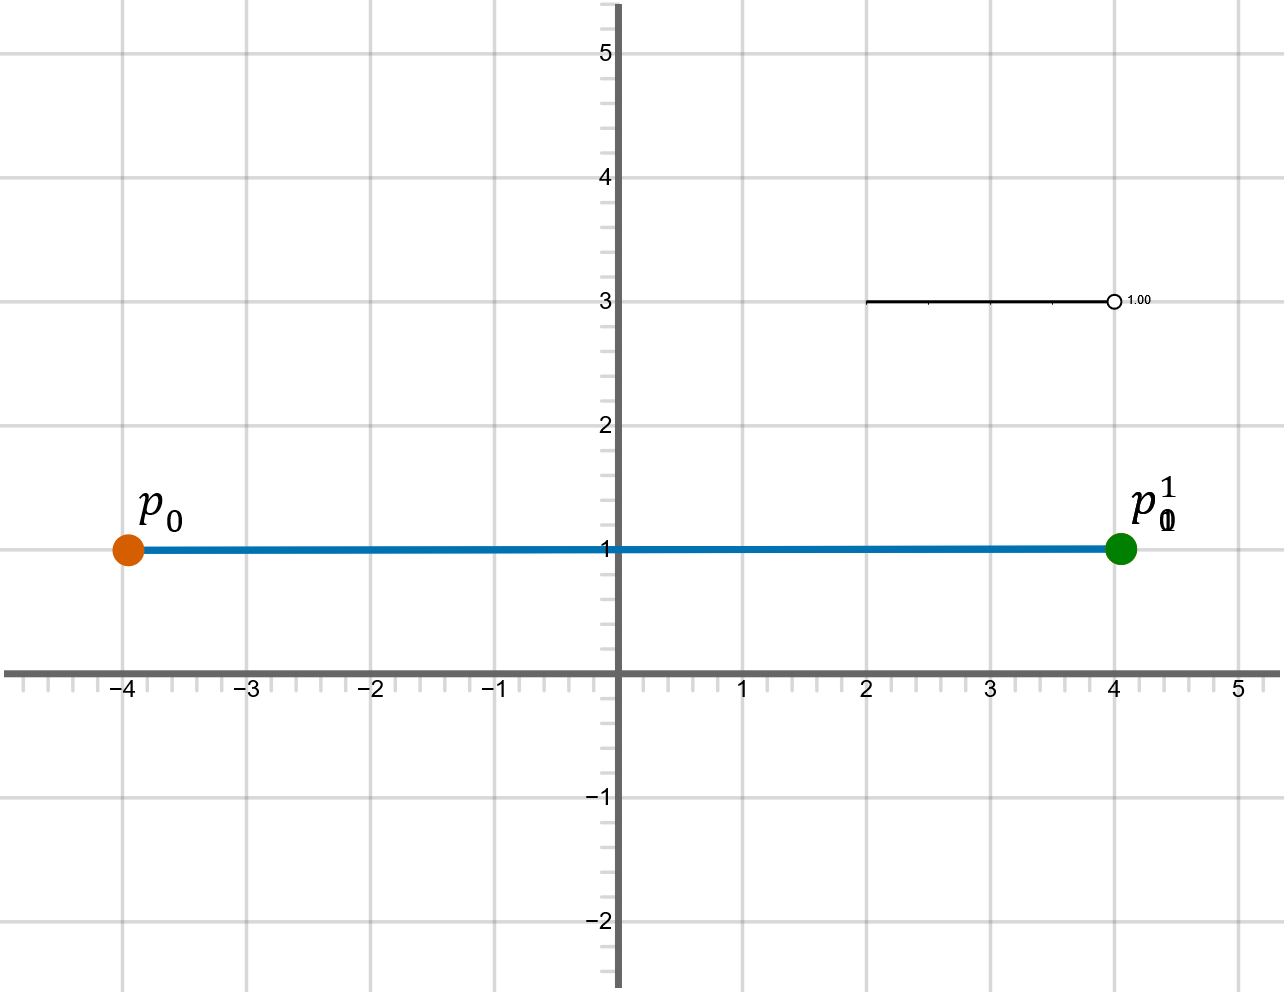
\includegraphics[width = \groupimagewidth]{images/decasteljau-n-1-t-1}}
        \caption{De Casteljaujev algoritem za $n=1$.}
        \label{fig:dec-alg-n1}
    \end{figure}
    \begin{figure}[h!]
        \captionsetup[subfigure]{labelformat=empty}
        \centering
        \subfloat[$t=0.25$]{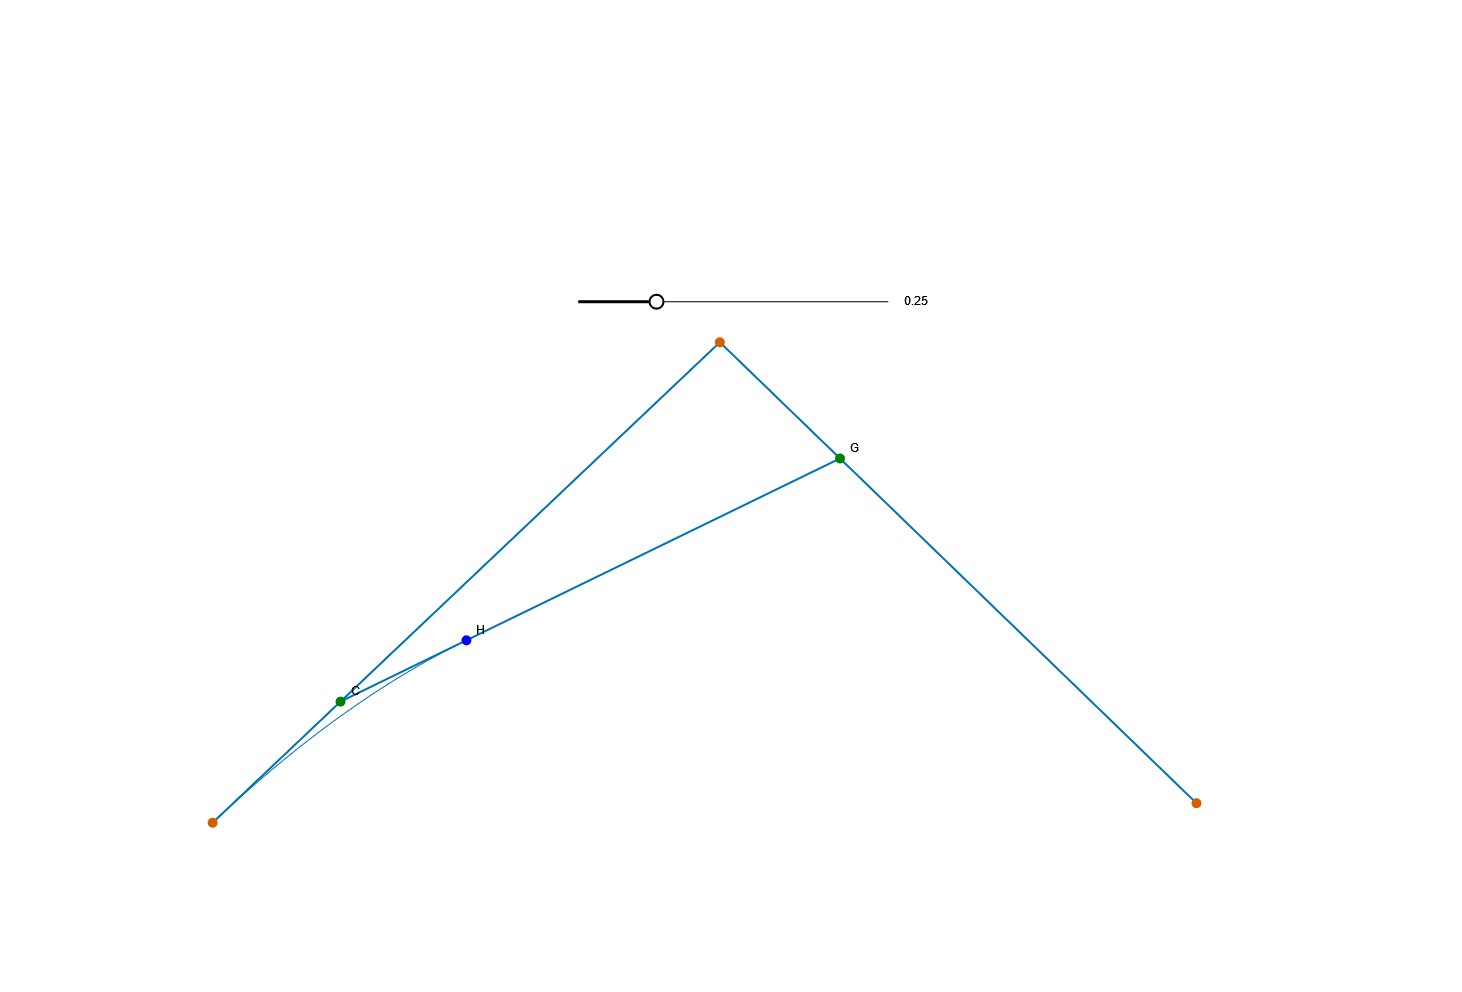
\includegraphics[width = \groupimagewidth]{images/decasteljau-n-2-t-025}}
        \qquad
        \subfloat[$t=0.5$]{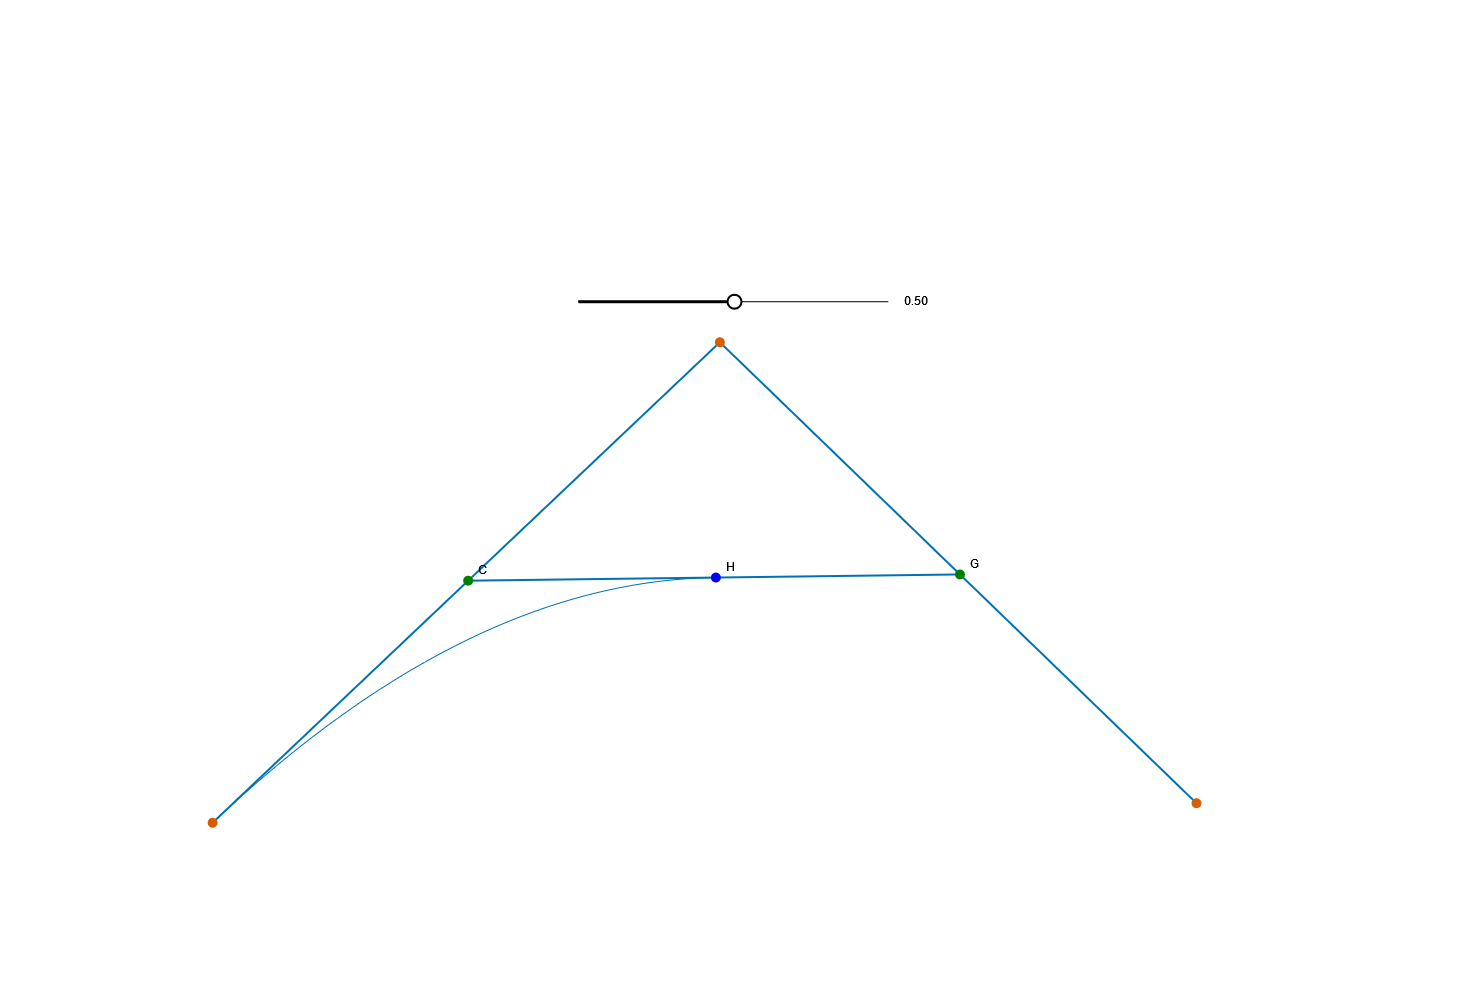
\includegraphics[width = \groupimagewidth]{images/decasteljau-n-2-t-05}}
        \\
        \subfloat[$t=0.75$]{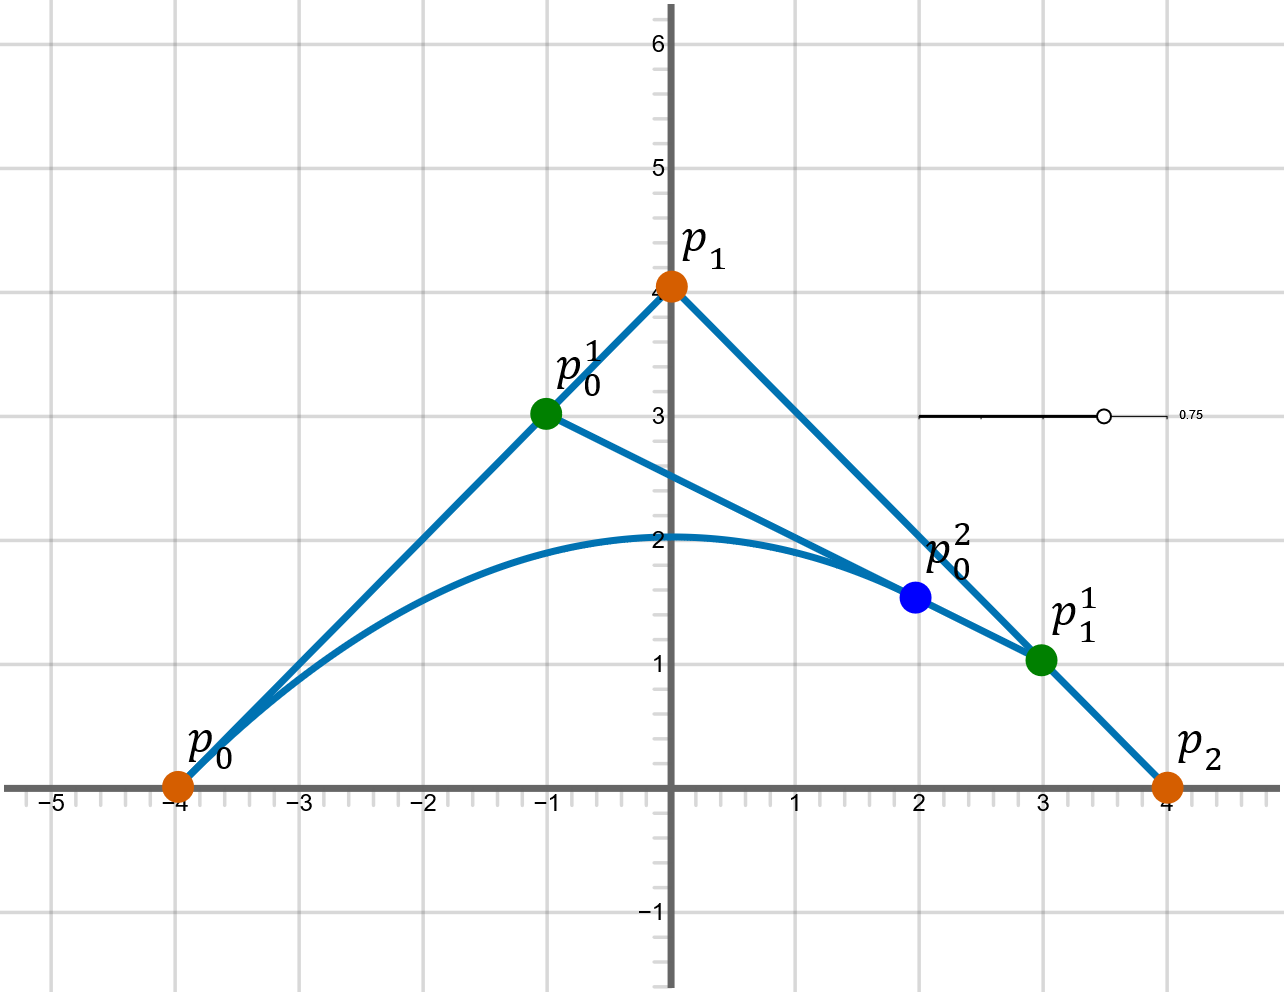
\includegraphics[width = \groupimagewidth]{images/decasteljau-n-2-t-075}}
        \qquad
        \subfloat[$t=1$]{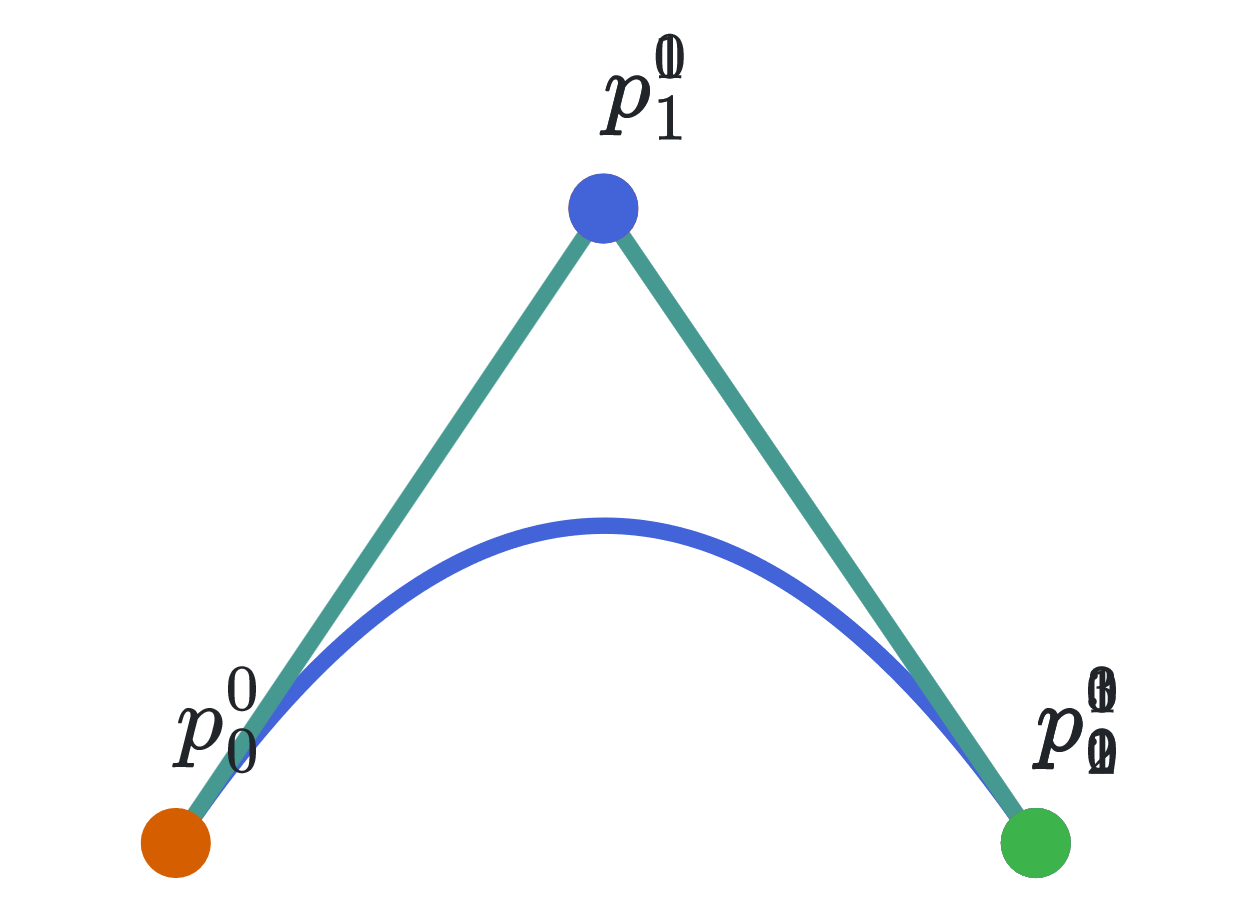
\includegraphics[width = \groupimagewidth]{images/decasteljau-n-2-t-1}}
        \caption{De Casteljaujev algoritem za $n=2$.}
        \label{fig:dec-alg-n2}
    \end{figure}
    \begin{figure}[h!]
        \captionsetup[subfigure]{labelformat=empty}
        \centering
        \subfloat[$t=0.25$]{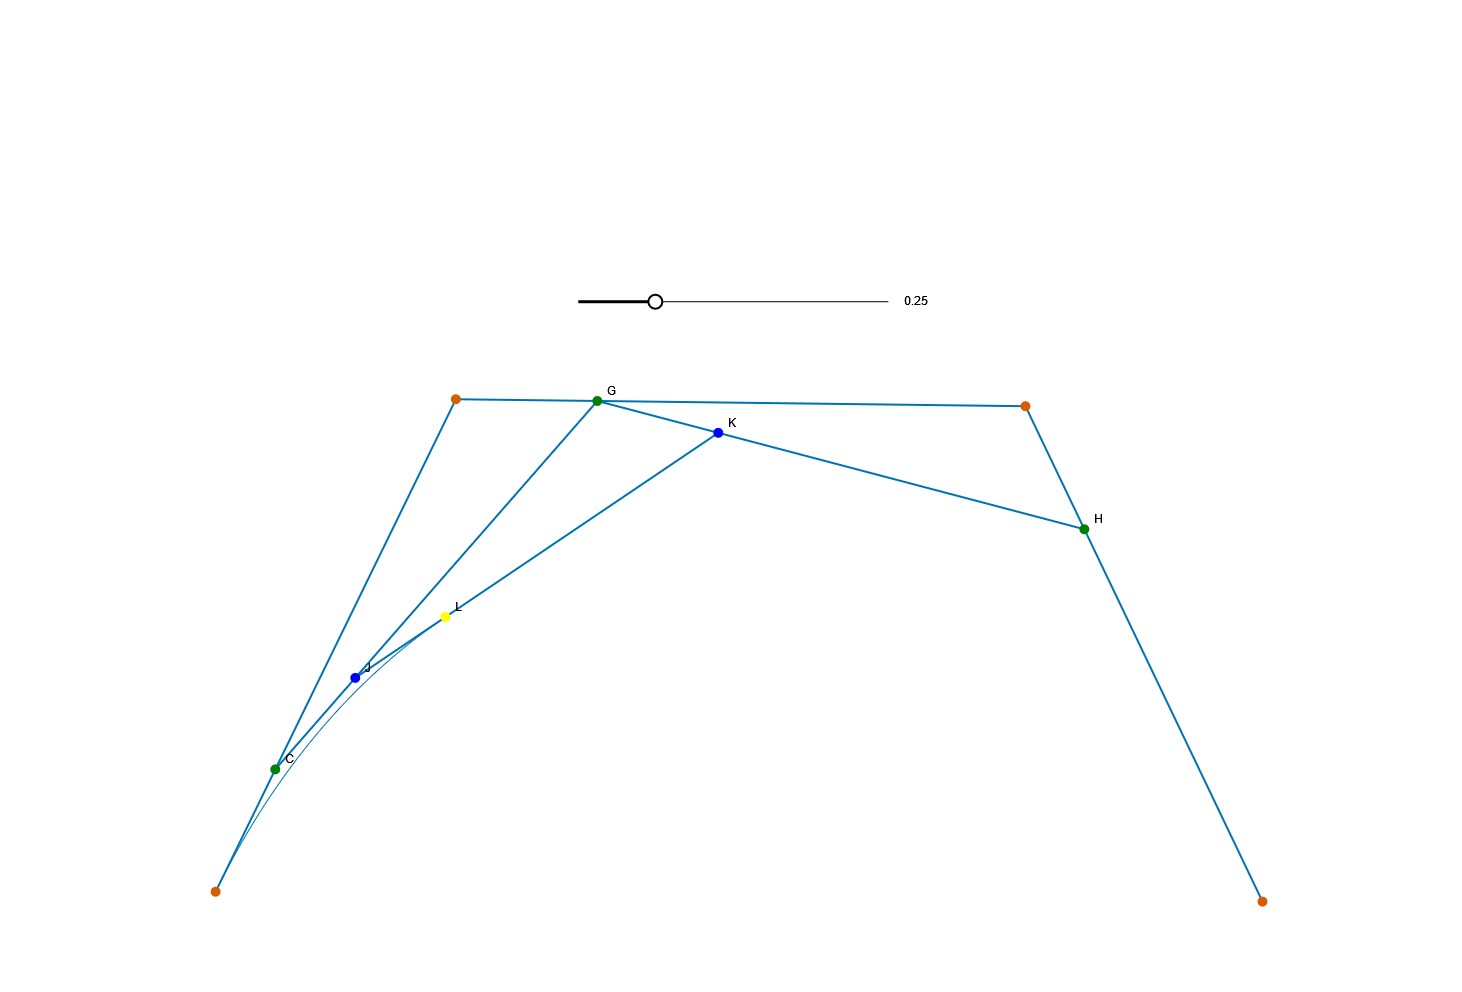
\includegraphics[width = \groupimagewidth]{images/decasteljau-n-3-t-025}}
        \qquad
        \subfloat[$t=0.5$]{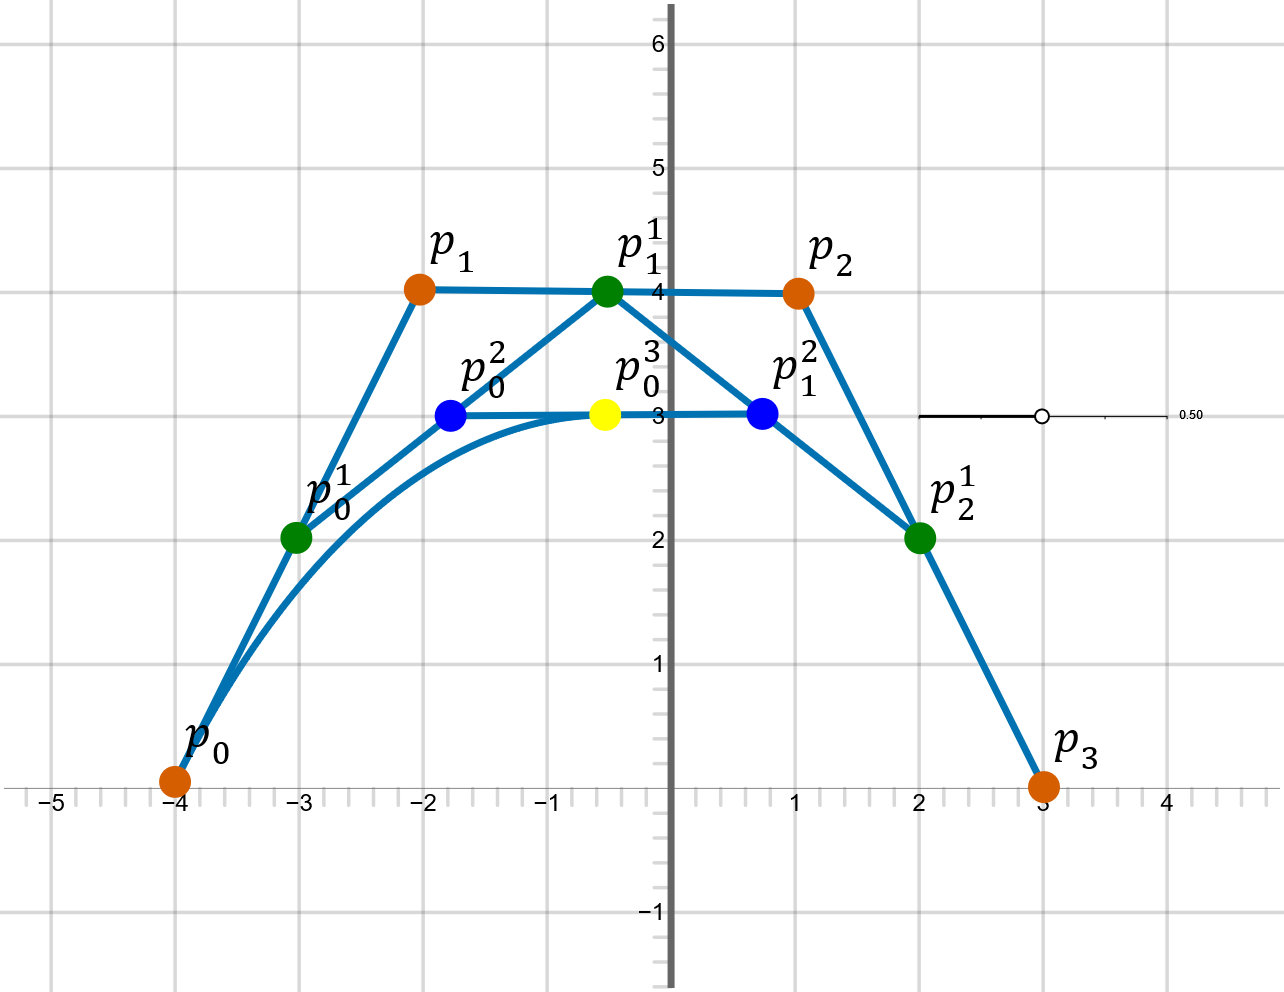
\includegraphics[width = \groupimagewidth]{images/decasteljau-n-3-t-05}}
        \\
        \subfloat[$t=0.75$]{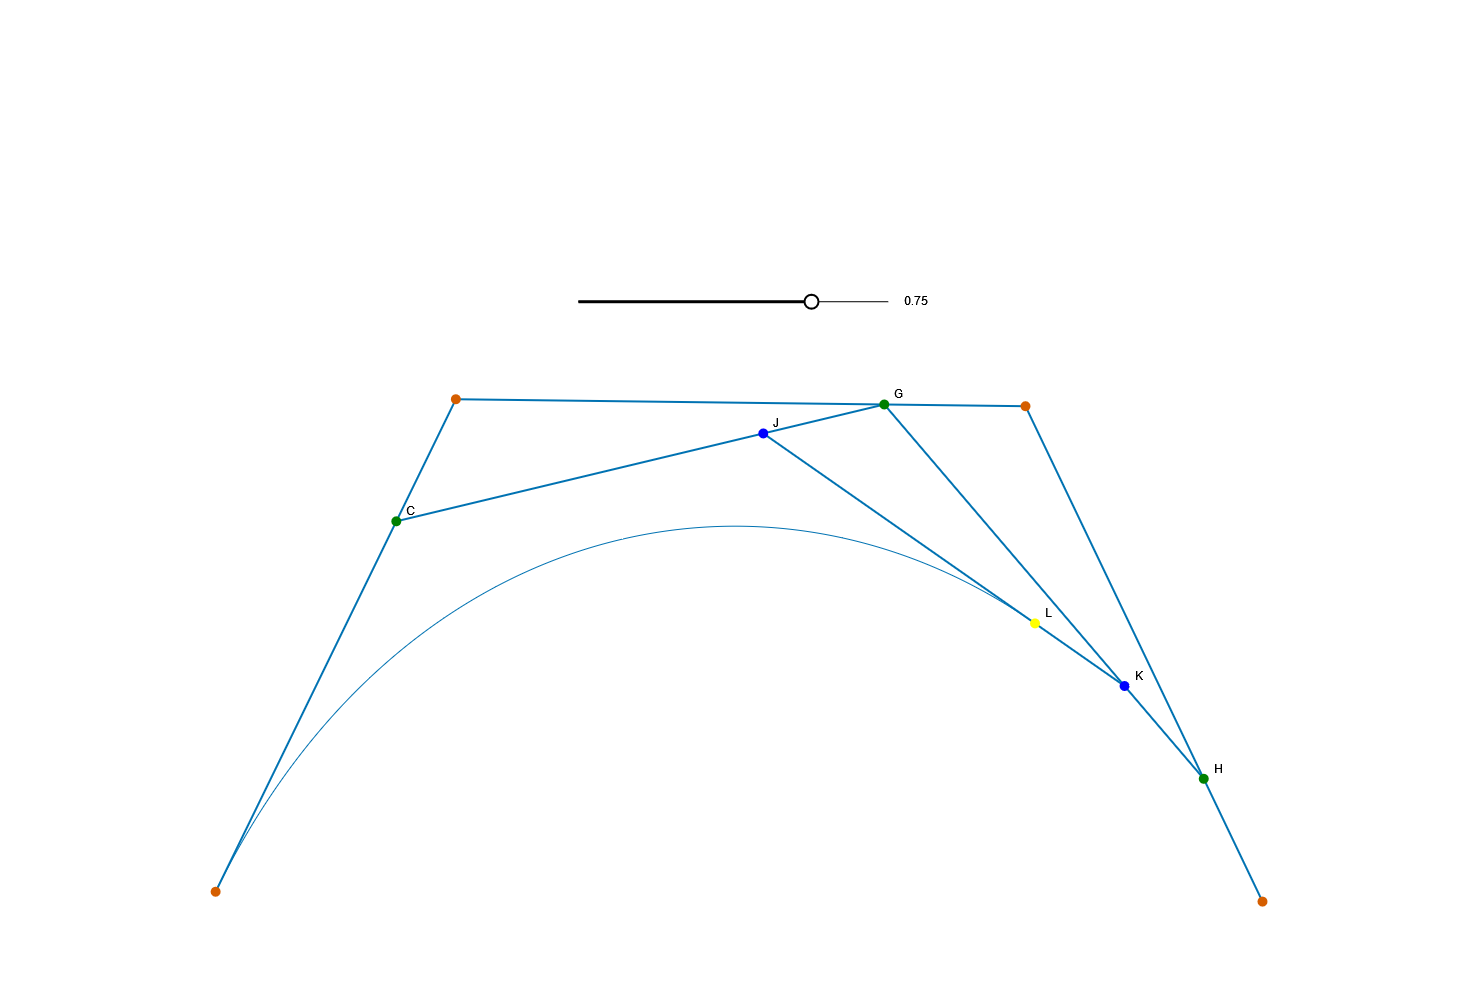
\includegraphics[width = \groupimagewidth]{images/decasteljau-n-3-t-075}}
        \qquad
        \subfloat[$t=1$]{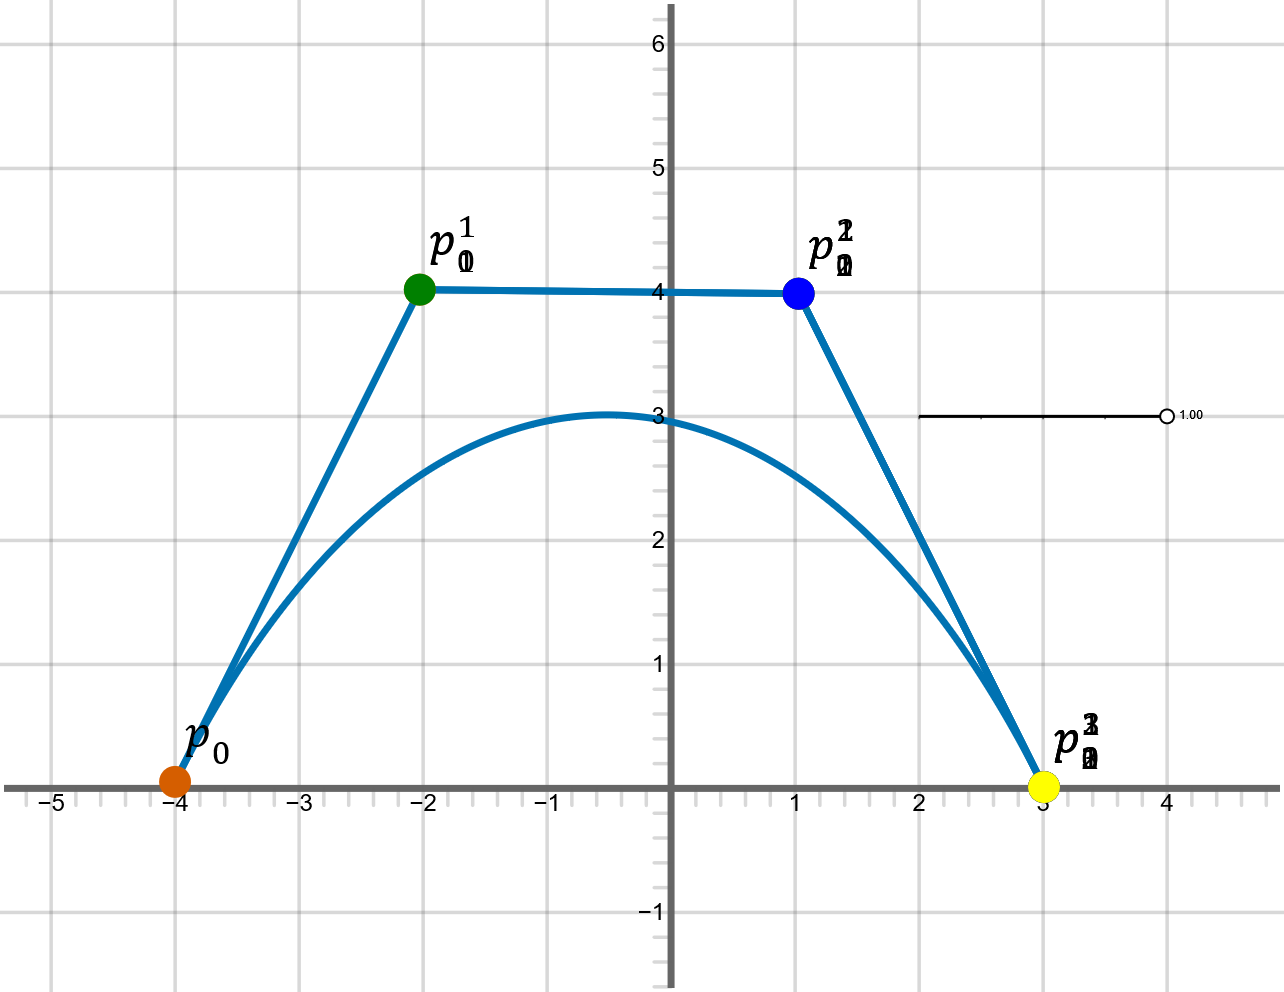
\includegraphics[width = \groupimagewidth]{images/decasteljau-n-3-t-1}}
        \caption{De Casteljaujev algoritem za $n=3$.}
        \label{fig:dec-alg-n3}
    \end{figure}
%    \begin{figure}[h!]
%        \captionsetup[subfigure]{labelformat=empty}
%        \centering
%        \subfloat[$t=0.25$]{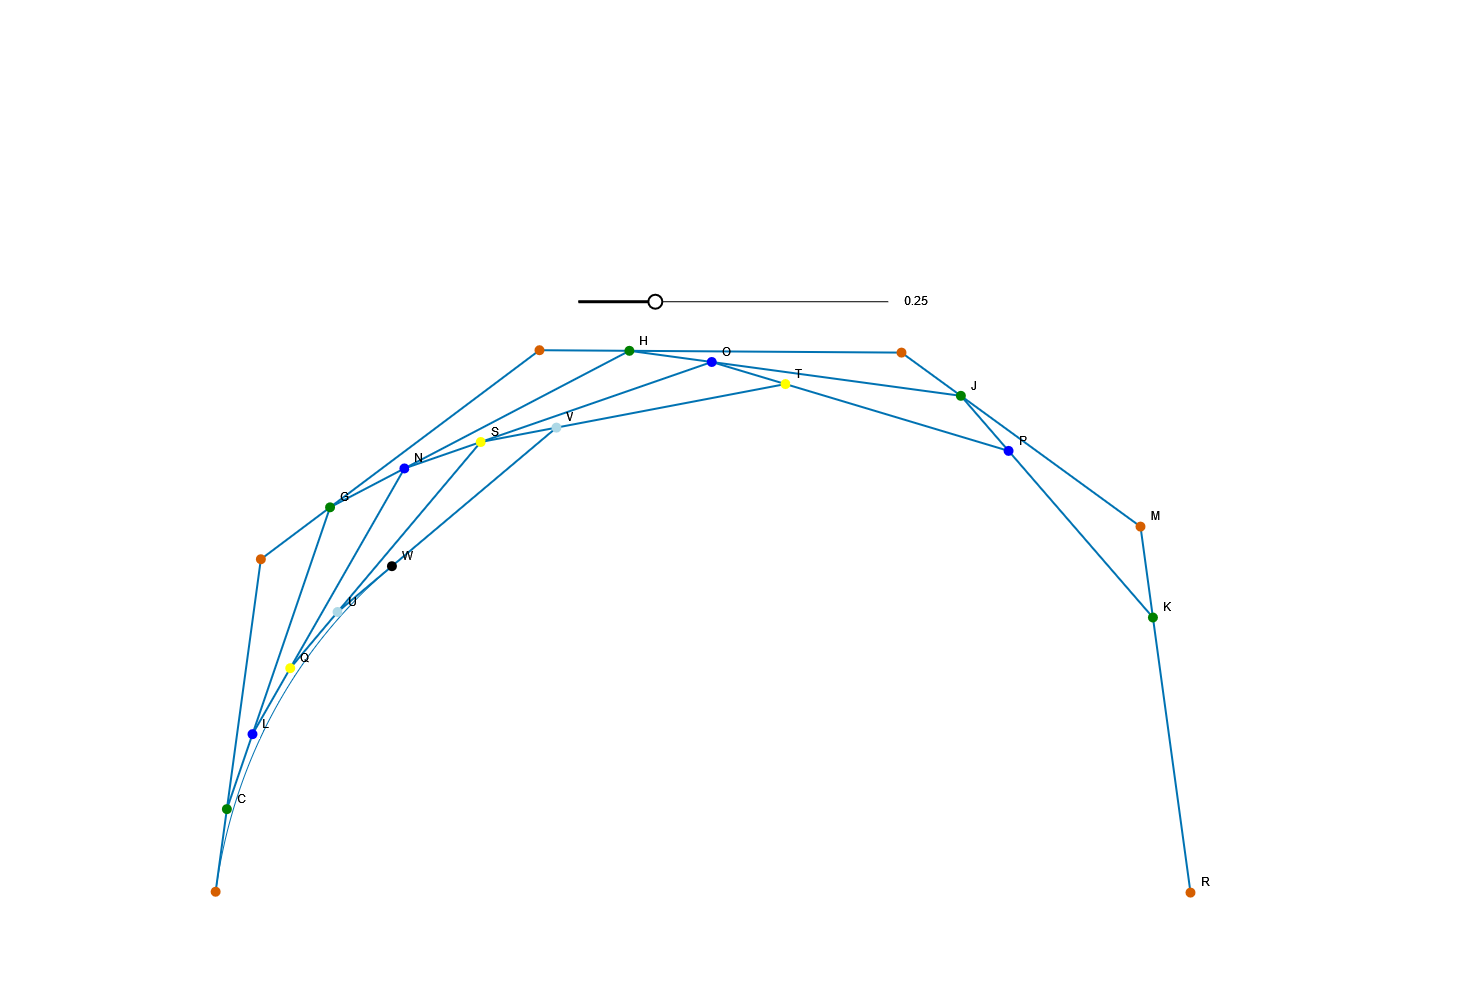
\includegraphics[width = \groupimagewidth]{images/decasteljau-n-5-t-025}}
%        \qquad
%        \subfloat[$t=0.5$]{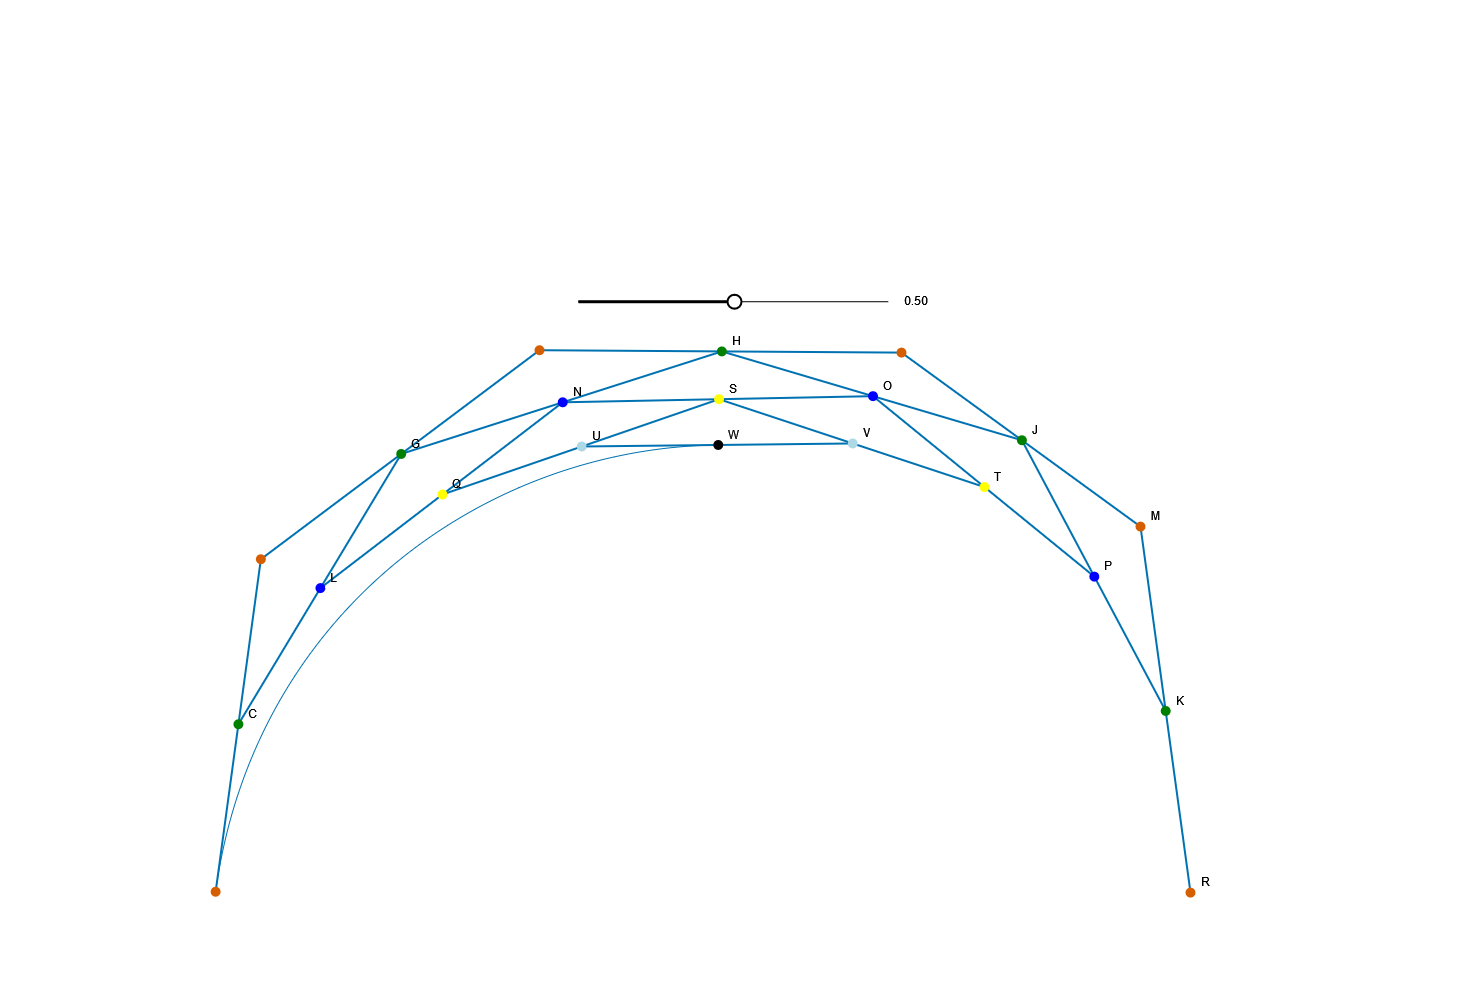
\includegraphics[width = \groupimagewidth]{images/decasteljau-n-5-t-05}}
%        \qquad
%        \subfloat[$t=0.75$]{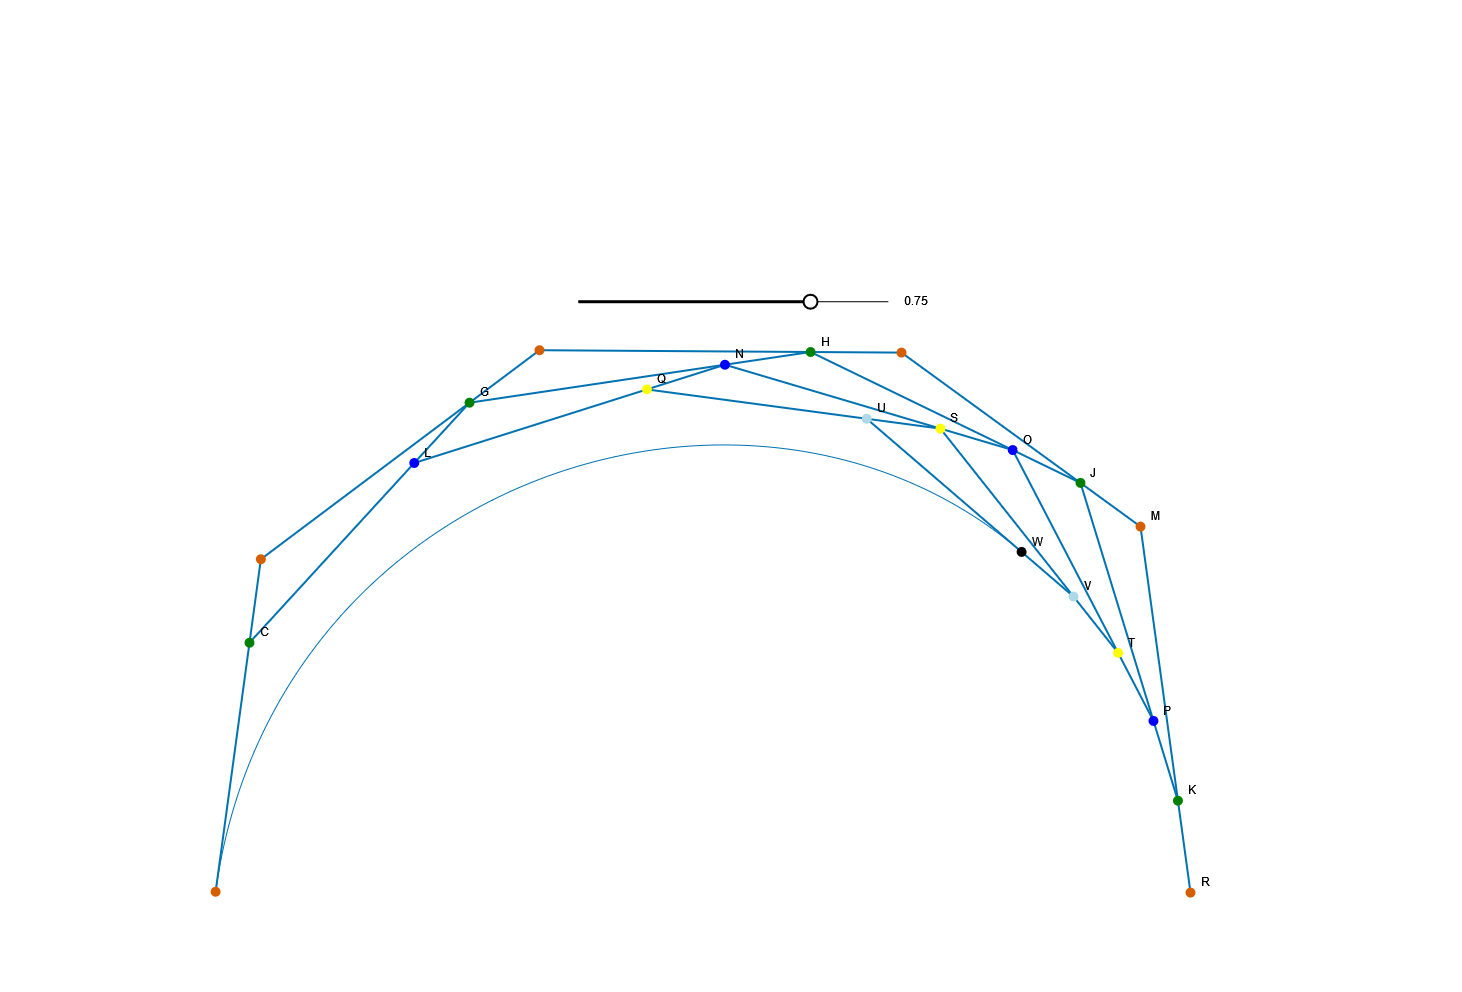
\includegraphics[width = \groupimagewidth]{images/decasteljau-n-5-t-075}}
%        \qquad
%        \subfloat[$t=1$]{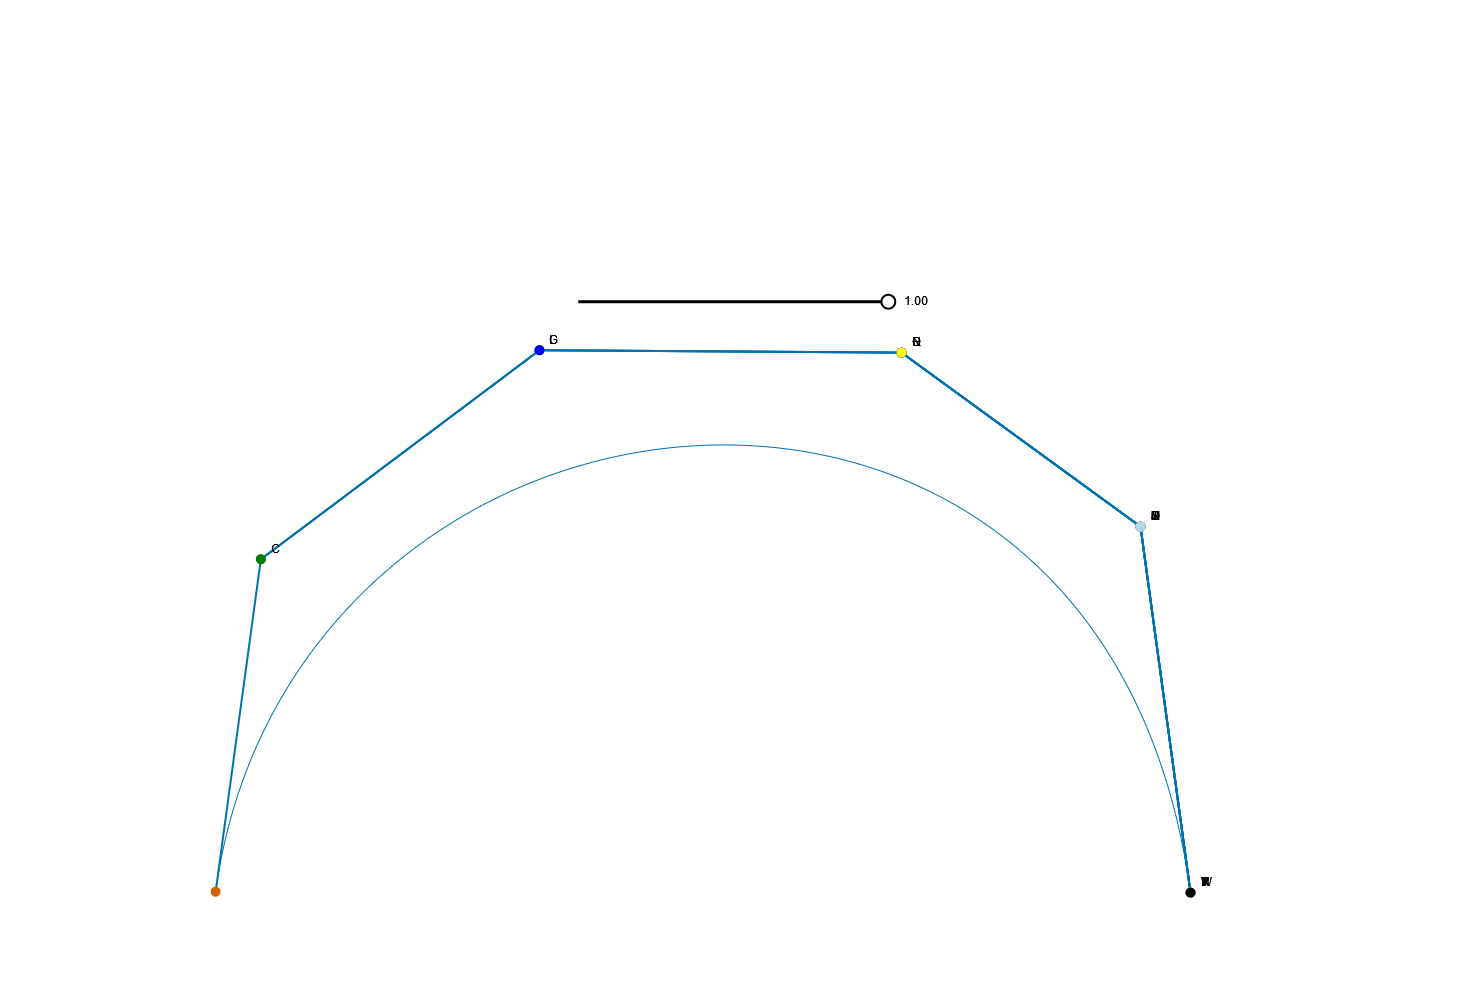
\includegraphics[width = \groupimagewidth]{images/decasteljau-n-5-t-1}}
%        \caption{De Casteljaujev algoritem za $n=5$}
%        \label{fig:dec-alg-n5}
%    \end{figure}

    \subsection{Subdivizija}
    V CAD in CAGD sistemih se mnogokrat zgodi, da uporabnik želi ohraniti le en del Bézierjeve krivulje.
    Naj bo to tisti del krivulje, ki ga dobimo tako, da za prvotno krivuljo parameter $t$ omejimo na interval $[0,t_0]$, za neko pozitivno realno število $t_0<1$.
    Ta del krivulje označimo z $B_{t_0-}$.
    Izkaže se, da lahko krivuljo $B_{t_0-}$ podamo kot Bézierjevo krivuljo s kontrolnimi točkami $\p_0^i(t_0)$ za $i=0,1,\ldots,n$, kjer točke $\p_0^i(t_0)$ dobimo iz de Casteljaujeve sheme pri $t=t_0$.
    Podobno se izkaže tudi to, da lahko preostali del krivulje, $B_{t_0+}$, podamo kot Bézierjevo krivuljo s kontrolnimi točkami $\p_i^i(t_0)$,  $i=0,1,\ldots,n$.
    Procesu deljenja krivulje na dva dela pravimo \textit{subdivizija}.
    Radovedni bralci lahko dokaz trditev najdejo v delu~\cite{farouki}.
    Primer si lahko ogledamo na sliki~\ref{fig:subdivizija}.
    \begin{figure}[h]
        \centering
        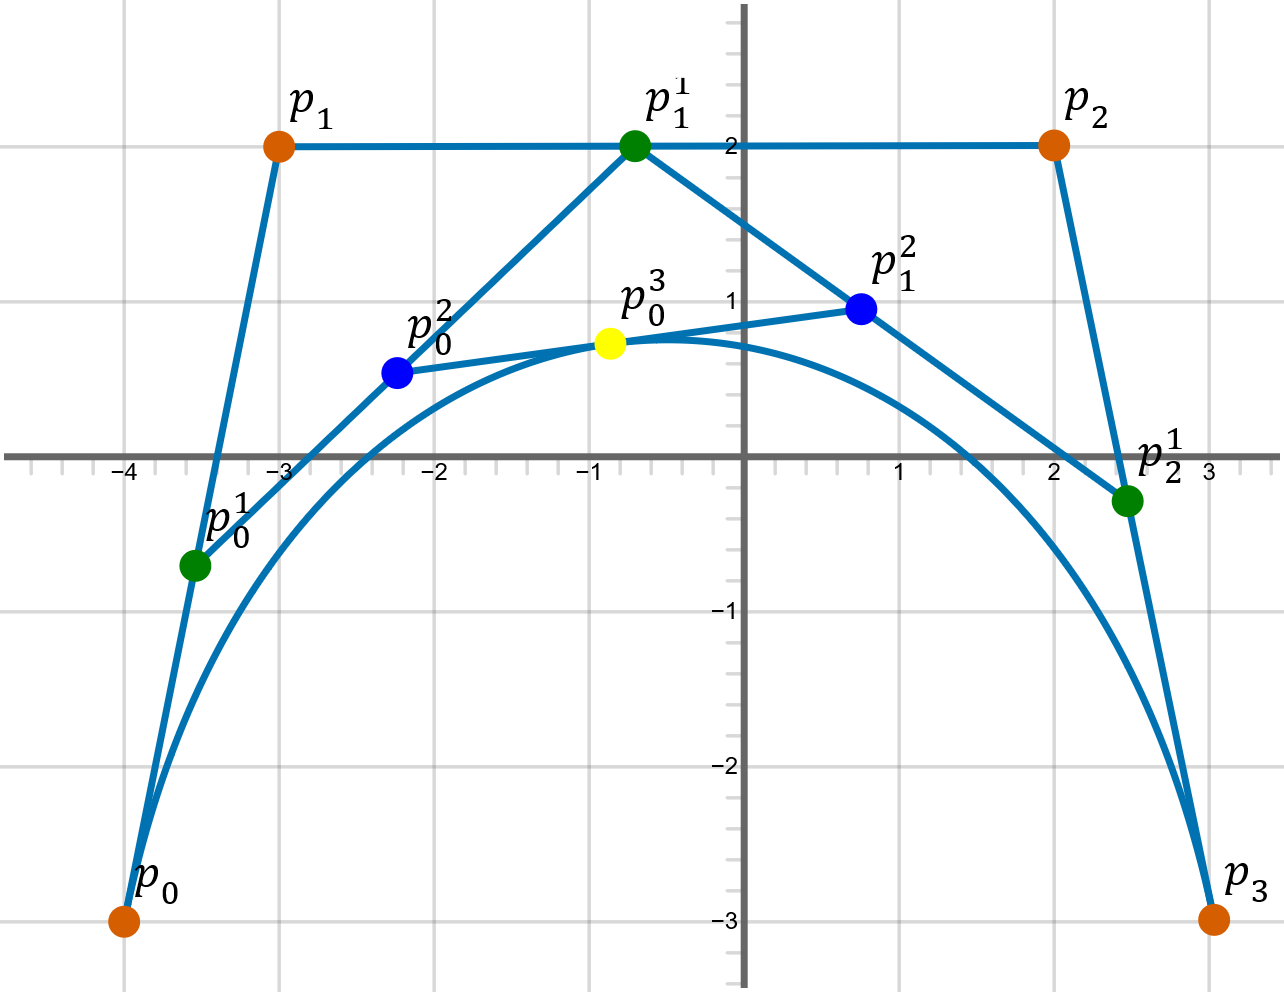
\includegraphics[width=\groupimagewidth]{images/subdivizija}
        \qquad
        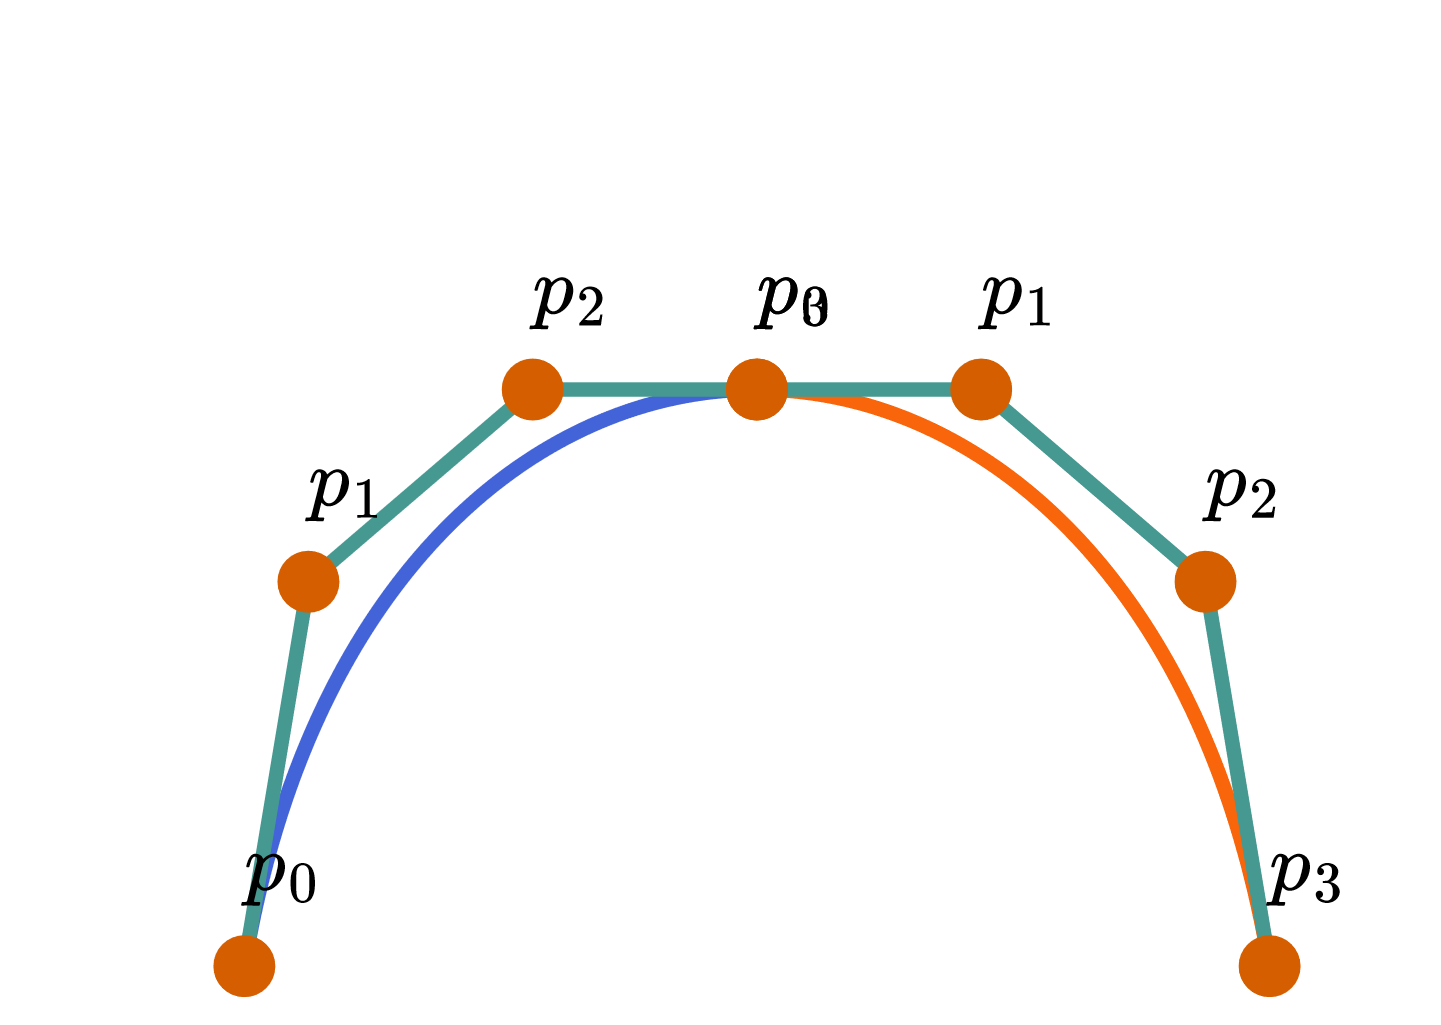
\includegraphics[width=\groupimagewidth]{images/subdivision-split}
        \caption{De Casteljaujeva shema pri $t=t_0$ razdeli krivuljo na dva dela, modrega, $B_{t_0-}$, in oranžnega, $B_{t_0+}$. }
        \label{fig:subdivizija}
    \end{figure}

    Če izberemo sedaj $t_0=\frac{1}{2}$ in krivuljo subdiviziramo, dobimo dve krivulji.
    Če subdivizijo nato na dobljenih krivuljah ponavljamo, dobimo po $k$ korakih $2^k$ krivulj.
    Na sliki~\ref{fig:subdivizija-ponavljanje} si lahko ogledamo postopek za prve tri korake.
    Opazimo, da so kontrolni poligoni dobljenih krivulj vse bližje krivulji.
    \begin{figure}[h]
        \captionsetup[subfigure]{labelformat=empty}
        \centering
        \subfloat[začetna krivulja]{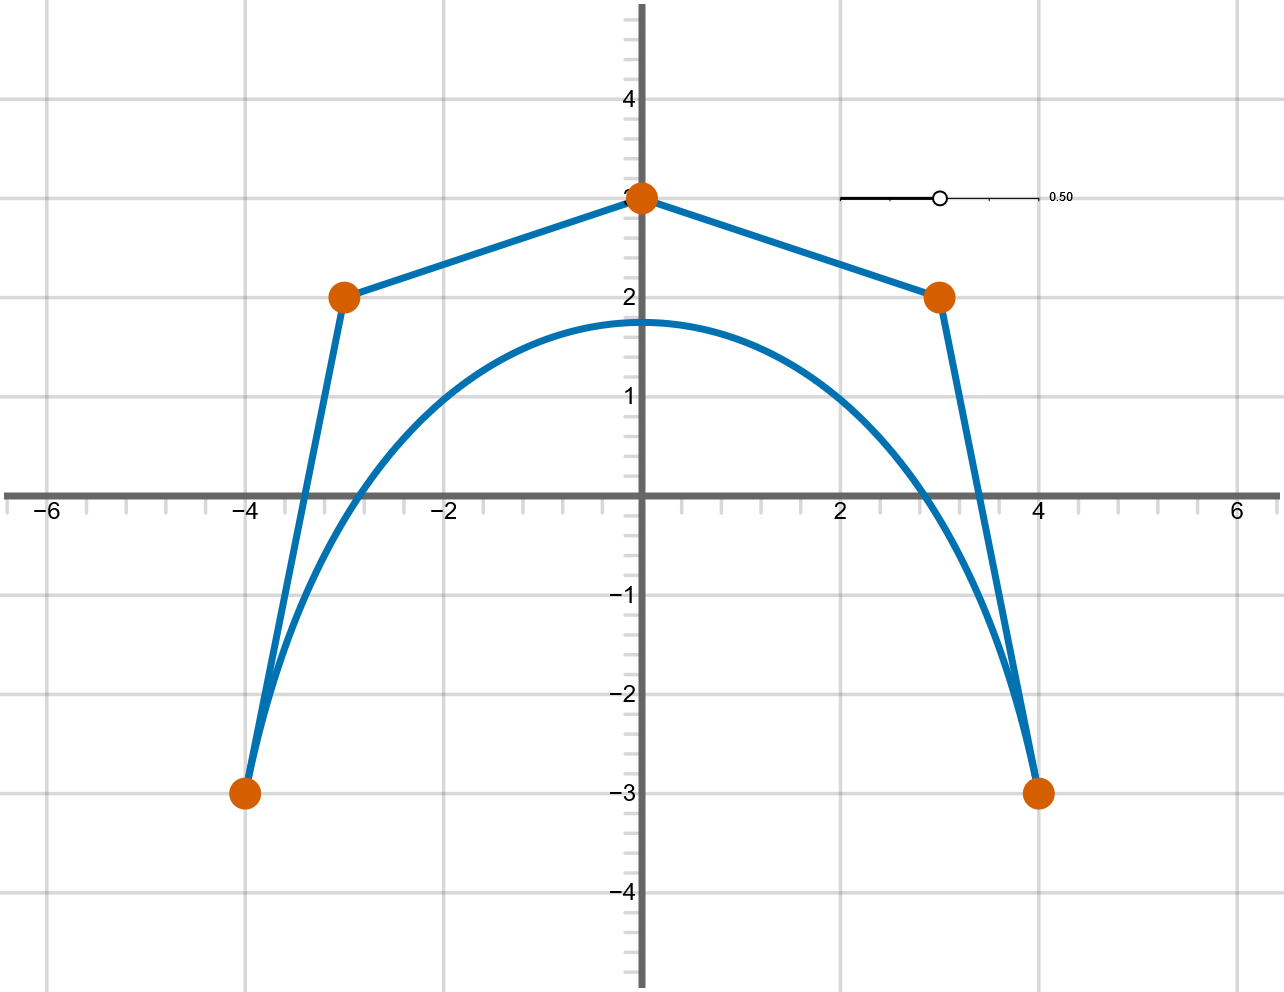
\includegraphics[width = \groupimagewidth]{images/subdivizija-k-0}}
        \qquad
        \subfloat[$2$ krivulji]{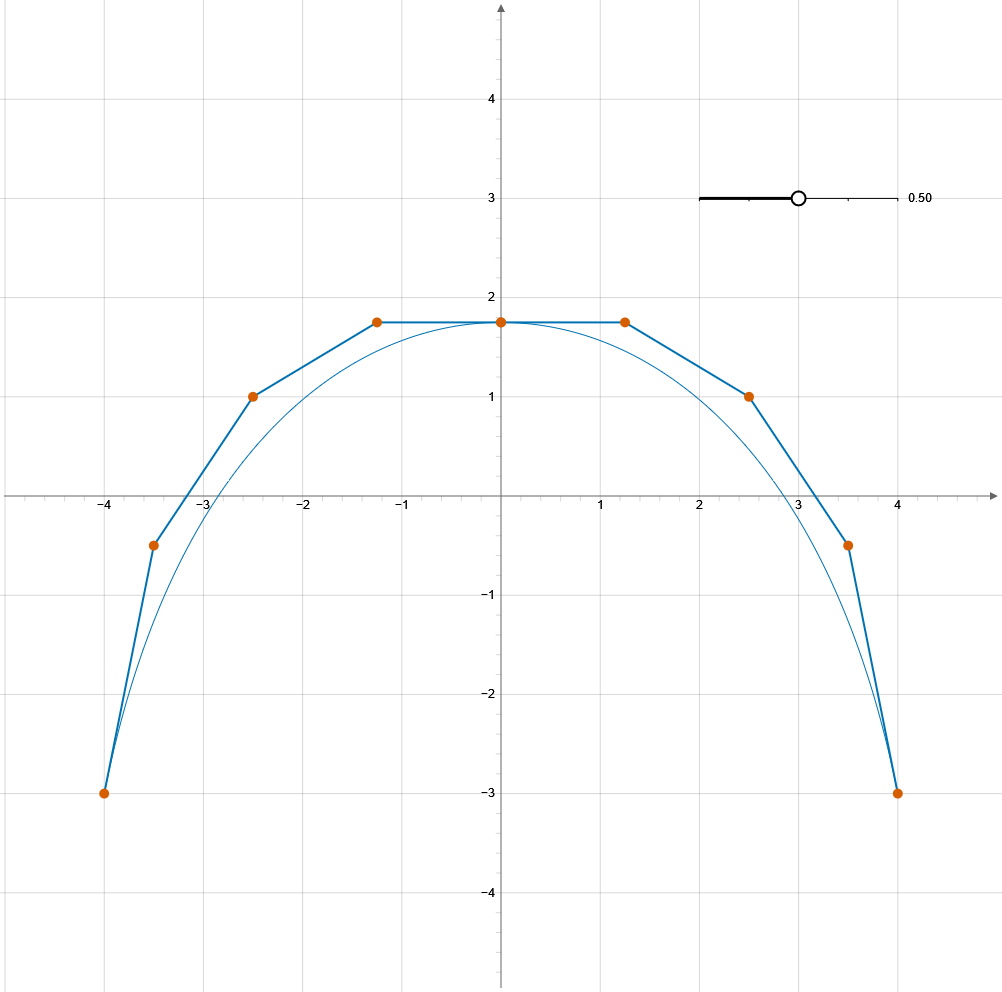
\includegraphics[width = \groupimagewidth]{images/subdivizija-k-1}}

        \subfloat[$4$ krivulje]{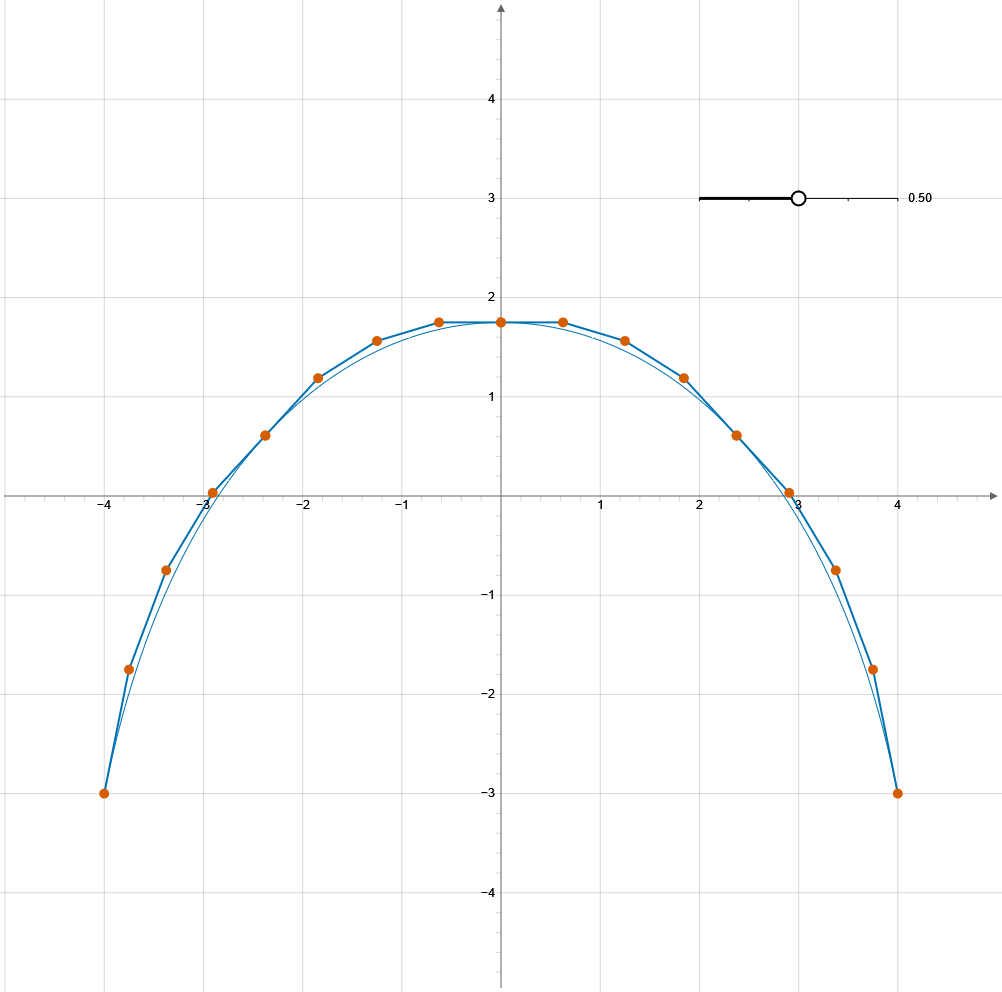
\includegraphics[width = \groupimagewidth]{images/subdivizija-k-2}}
        \qquad
        \subfloat[$8$ krivulj]{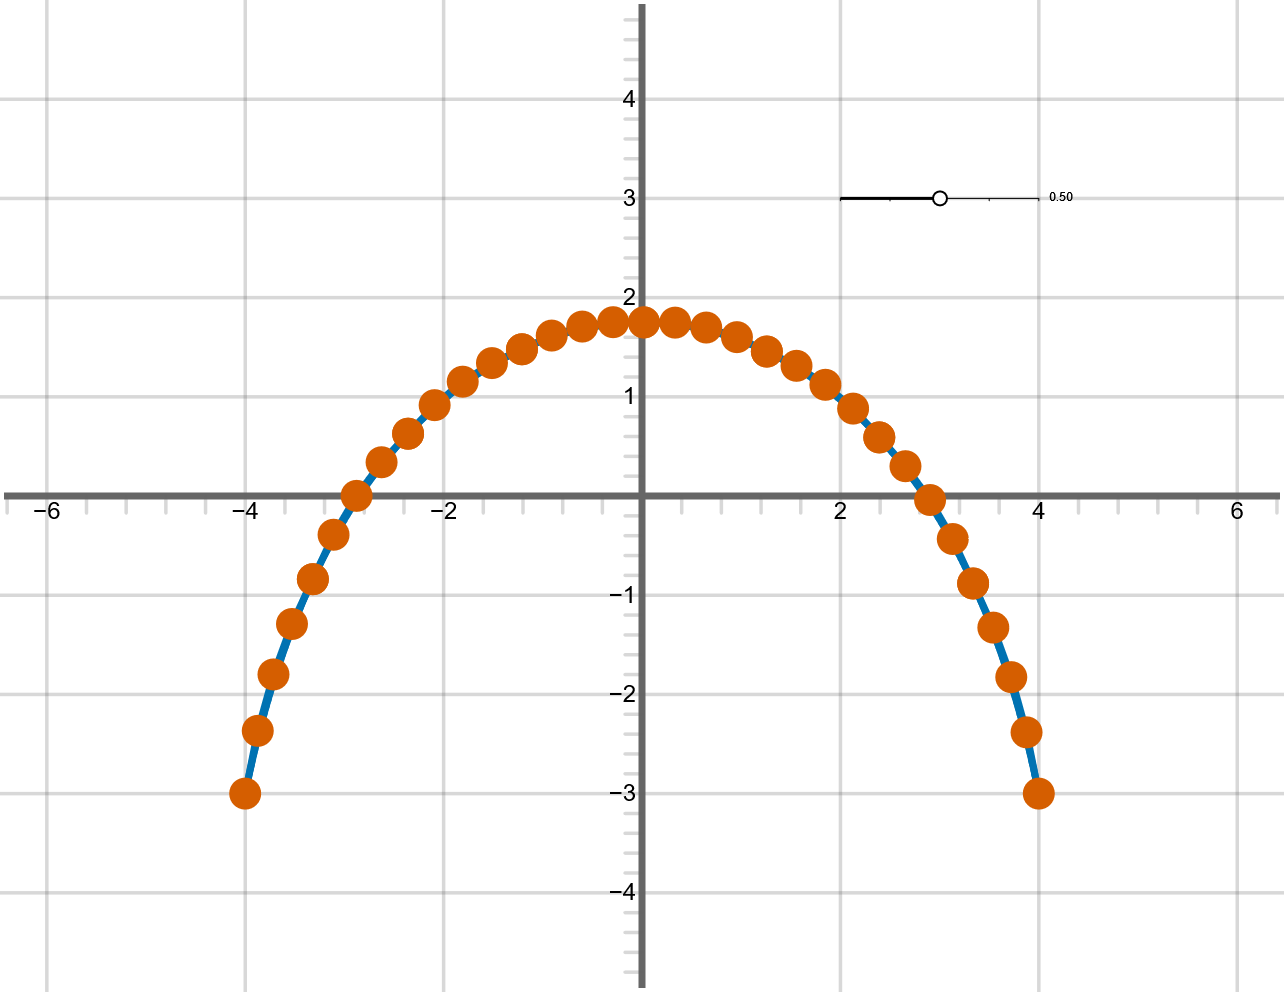
\includegraphics[width = \groupimagewidth]{images/subdivizija-k-3}}
        \caption{Ponavljanje subdivizije.}
        \label{fig:subdivizija-ponavljanje}
    \end{figure}


%    \begin{dokaz}
%        \begin{align*}
%            B_{t_0}(t) = B(t_{0}t) &= \sum_{i=0}^{n}\mathbf{p}_{i}\binom{n}{i}(t_{0}t)^i(1-tt_0)^{n-i}\\
%            &= \sum_{i=0}^{n}\mathbf{p}_{i}\binom{n}{i}(t_{0}t)^i \sum_{j=0}^{n-i} \binom{n-i}{j}(-tt_0)^{j}  \\
%            &= \sum_{i=0}^{n}\mathbf{p}_{i}\binom{n}{i}(tt_0)^i \sum_{j=0}^{n-i} \binom{n-i}{j}(-t)^{j}(t_0)^{j}\\
%            &= \sum_{i=0}^{n}\mathbf{p}_{i}\binom{n}{i}(tt_0)^i \sum_{j=0}^{n-i} \binom{n-i}{j}(-t)^{j}(t_0)^{j}
%        \end{align*}
%        Želimo dobiti
%
%        \begin{align*}
%            \sum_{i=0}^{n}\p_{0}^i(t_0)\binom{n}{i}t^i(1-t)^{n-i} = \sum_{i=0}^{n}\binom{n}{i}t^i(1-t)^{n-i}  \sum_{j=0}^{n-i} \binom{n-i}{j}t_0^j(1-t_0)^{n-i-j}  \p_{j}
%        \end{align*}
%
%    \end{dokaz}

    \subsection{Ekstrapolacija}\label{subsec:ekstrapolacija}
    Ker so Bernsteinovi bazni polinomi definirani za vsa realna števila $t$, lahko Bézierjeve krivulje rišemo tudi izven domene $[0,1]$.
    Recimo, da želimo neko Bézierjevo krivuljo risati na domeni $[0,t_0]$, kjer je $t_0>1$.
    Bézierjevo krivuljo na domeni $[0,t_0]$ lahko predstavimo kot Bézierjevo krivuljo na domeni $[0,1]$.
    Pri tem kontrolne točke krivulje preberemo iz de Casteljaujeve sheme, kakor smo to storili za točke krivulje  $B_{t_0-}$ v prejšnjem razdelku, krivulja $B_{t_0+}$ pa predstavlja ekstrapoliran del krivulje.
    Na sliki~\ref{fig:ekstrapolacija} lahko na prvem grafu vidimo risanje krivulje izven intervala $[0,1]$, na drugem pa ekstrapolirano krivuljo.
    \begin{figure}[h]
        \captionsetup[subfigure]{labelformat=empty}
        \centering
        \subfloat[pred ekstrapolacijo]{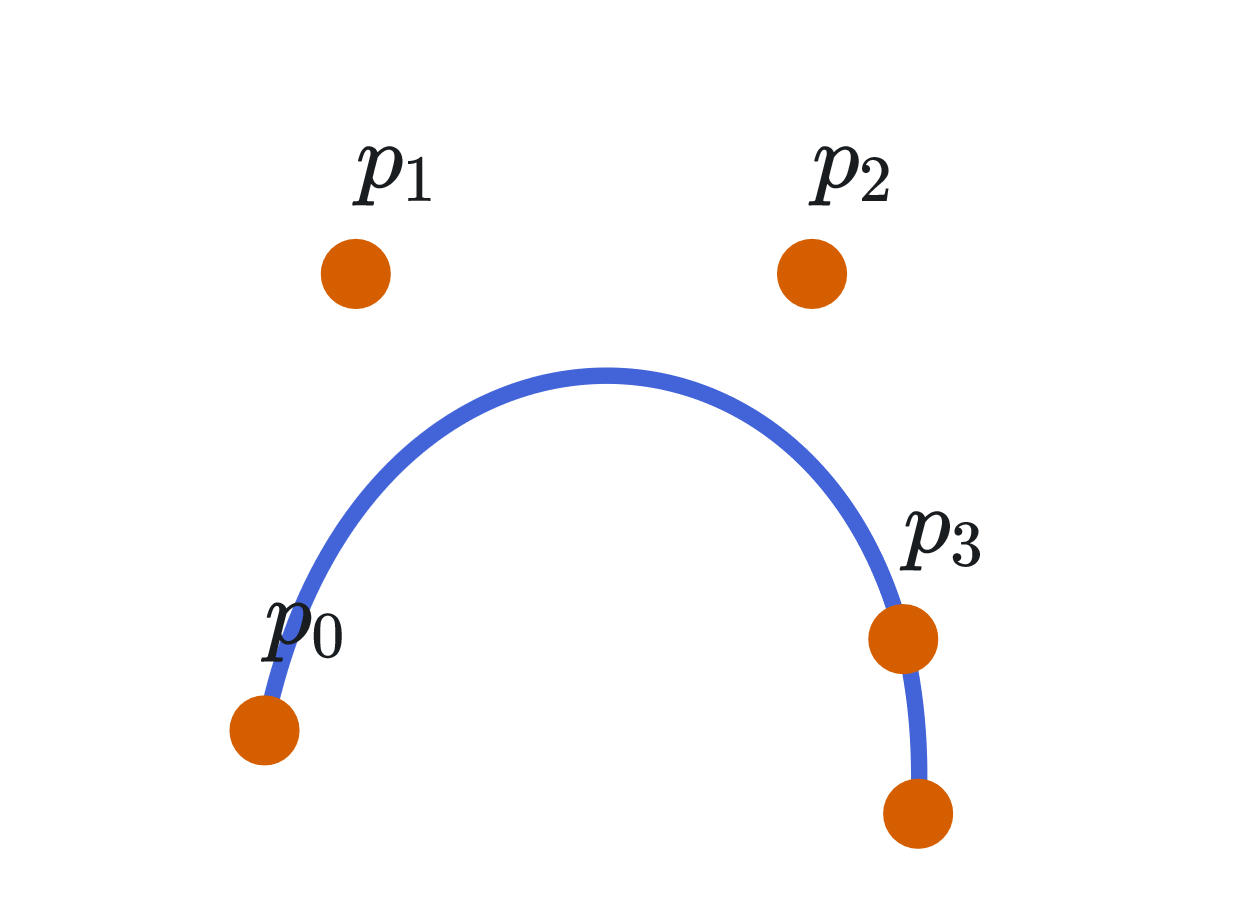
\includegraphics[width = \groupimagewidth]{images/extrapolation-before}}
        \qquad
        \subfloat[po ekstrapolaciji]{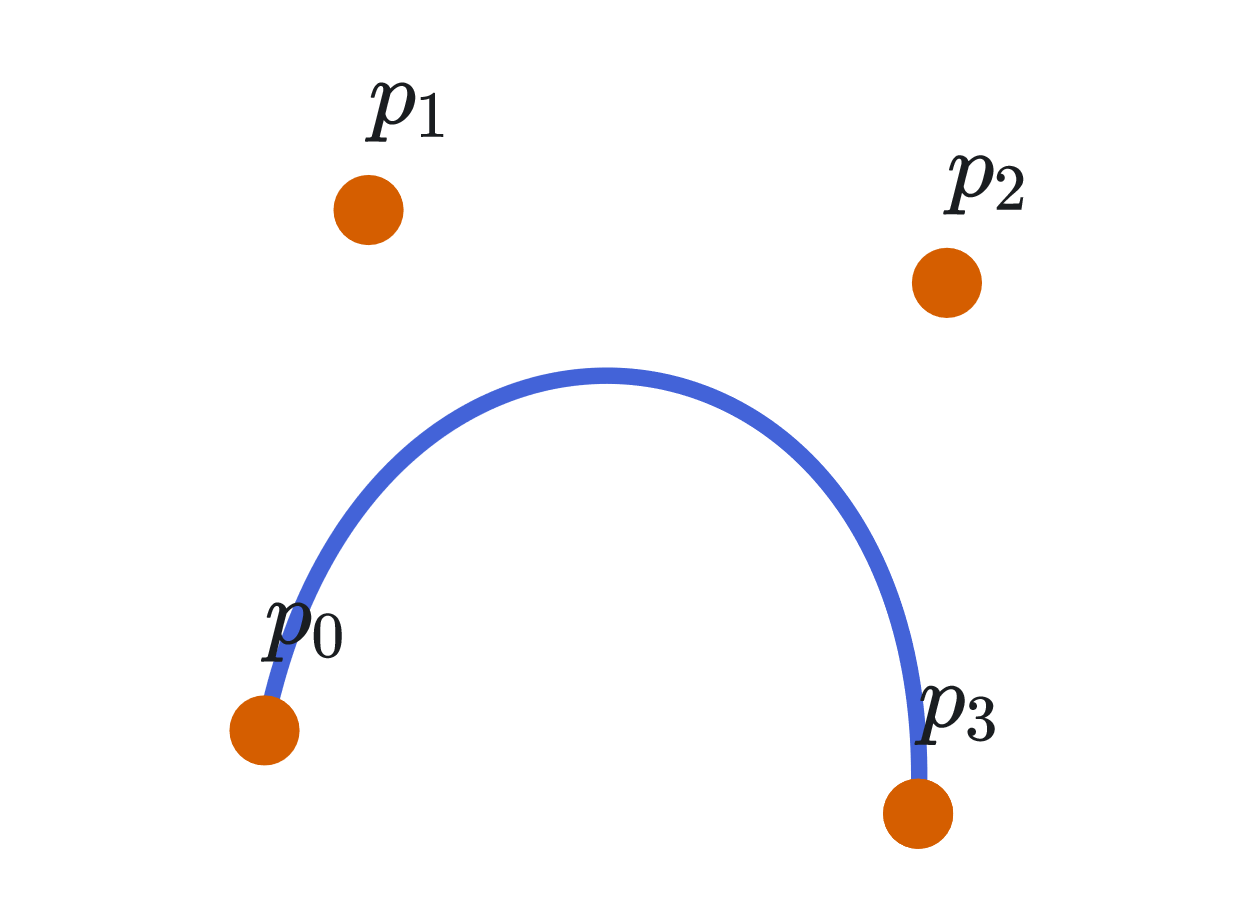
\includegraphics[width = \groupimagewidth]{images/extrapolation-after}}
        \caption{Ekstrapolacija Bézierjeve krivulje.}
        \label{fig:ekstrapolacija}
    \end{figure}

    \subsection{Višanje stopnje}
    Nekateri algoritmi v CAD in CAGD sistemih za vhod potrebujejo dve Bézierjevi krivulji iste stopnje
    Recimo, da imamo Bézierjevo krivuljo $\B$ stopnje $n$, ki jo želimo predstaviti kot Bézierjevo krivuljo stopnje $n+1$.
    Upoštevajoč $1-t+t=1$, lahko parametrizacijo krivulje $\B$ zapišemo tudi kot
    \begin{align}
        \B(t) = (1-t)\B(t)+t\B(t) = \sum_{i=0}^{n}\mathbf{p}_{i}(1-t)B_i^n(t) +\sum_{i=0}^{n}\mathbf{p}_{i}tB_i^n(t). \label{eq:visanje-param}
    \end{align}
    Če sedaj zvezi za Bernsteinove bazne polinome
    \begin{align*}
    (1-t)
        B_i^n(t) &= & \frac{n+1-i}{n+1} \binom{n+1}{i}&t^i(1-t)^{n+1-i} & &=\frac{n+1-i}{n+1}B_{i}^{n+1}(t), \\
        % &= \frac{n!}{(n-i)!i!}t^i(1-t)^{n+1-i}   &=\frac{n+1-i}{n+1}\frac{(n+1)!}{(n+1-i)!i!}t^i(1-t)^{n+1-i}
        tB_i^n(t) &= & \frac{i+1}{n+1}\frac{(n+1)!}{(n-i)!(i+1)!}&t^{i+1}(1-t)^{n+1-i-1} & &= \frac{i+1}{n+1}B_{n+1}^{n+1}(t),
        %t\binom{n}{i}t^i(1-t)^{n-i} \\
        %&= \frac{n!}{(n-i)!i!}t^{i+1}(1-t)^{n+1-i-1} \\
    \end{align*}
    vstavimo v izraz~\eqref{eq:visanje-param}, dobimo
    \begin{align*}
        \B(t) &= \sum_{i=0}^{n}\mathbf{p}_{i}\frac{n+1-i}{n+1}B_{i}^{n+1}(t) +\sum_{i=0}^{n}\mathbf{p}_{i}\frac{i+1}{n+1}B_{i+1}^{n+1}(t)\\
        &= \sum_{i=0}^{n}\mathbf{p}_{i}\frac{n+1-i}{n+1}B_{i}^{n+1}(t) +\sum_{i=1}^{n+1}\mathbf{p}_{i-1}\frac{i}{n+1}B_{i}^{n+1}(t).
%&=\mathbf{p}_{0} + \sum_{i=1}^{n}\left(\mathbf{p}_{i}\frac{n+1-i}{n+1} + \mathbf{p}_{i-1}\frac{i}{n+1}\right)B_{i}^{n+1}(t)+\mathbf{p}_{n}.
    \end{align*}
    Od tod sledi, da lahko krivuljo $\B$ predstavimo kot Bézierjevo krivuljo stopnje $n+1$ s kontrolnimi točkami \[\mathbf{c}_0=\p_0, \quad \mathbf{c}_i=\mathbf{p}_{i}\frac{n+1-i}{n+1} + \mathbf{p}_{i-1}\frac{i}{n+1},\quad \mathbf{c}_{n+1}=\p_n. \]
    Oglejmo si kako višanje stopnje poteka na neki dani krivulji.
    Na sliki~\ref{fig:višanje} je na prvem grafu narisana Bézierjeva krivulja stopnje $3$.
    Na drugem grafu, smo stopnjo krivulje zvišali za $1$, na tretjem in četrtem grafu pa smo naredili $10$ oziroma $20$ višanj stopnje začetne krivulje.
    Krivulja je na vseh grafih enaka, imamo le več kontrolnih točk.
    Opaziti je tudi možno, da so kontrolne točke z vsakim višanjem stopnje bližje začetni krivulji, kontrolni poligon pa se vedno bolj prilega začetni krivulji.
    \begin{figure}[h]
        \captionsetup[subfigure]{labelformat=empty}
        \centering
        \subfloat[začetna krivulja]{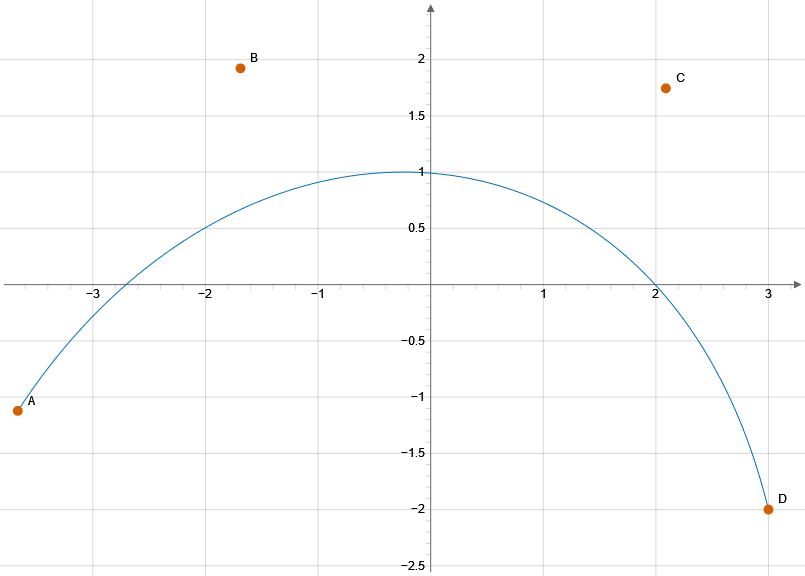
\includegraphics[width = \groupimagewidth]{images/dvig-prej}}
        \qquad
        \subfloat[eno višanje]{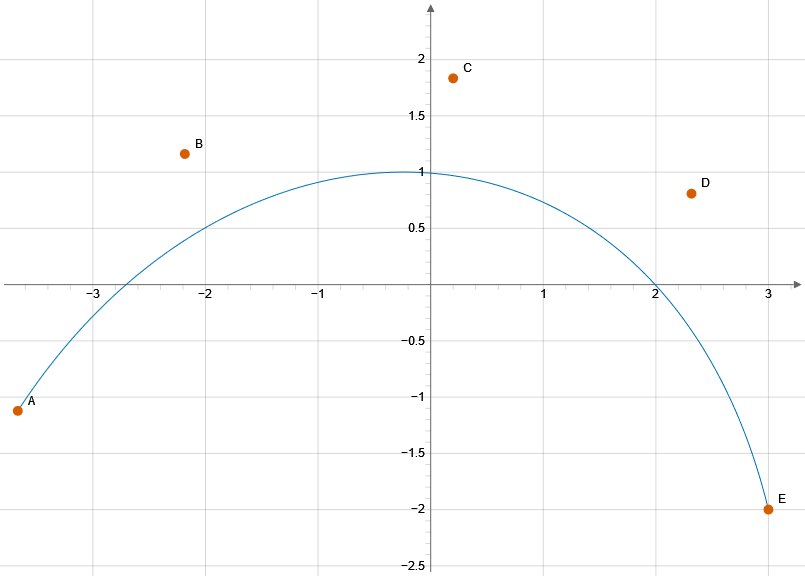
\includegraphics[width = \groupimagewidth]{images/dvig-po}} \\
        \subfloat[10 višanj]{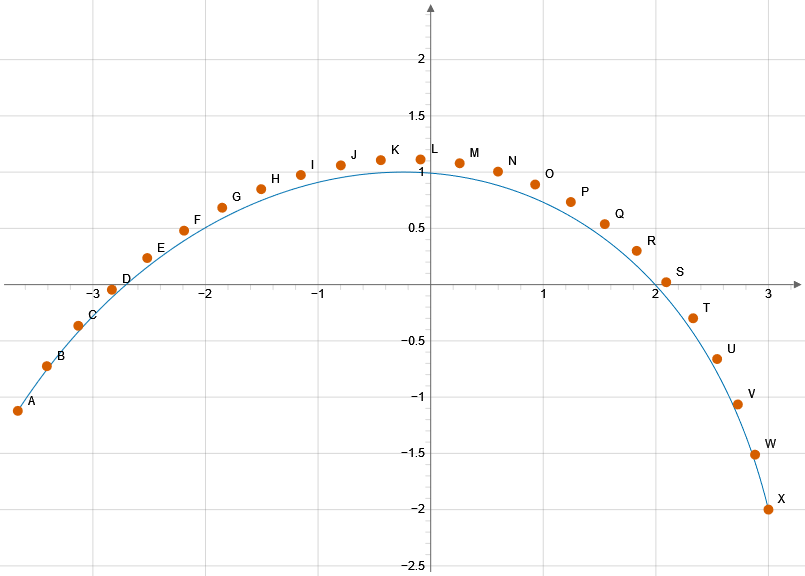
\includegraphics[width = \groupimagewidth]{images/dvig-n}}
        \qquad
        \subfloat[20 višanj]{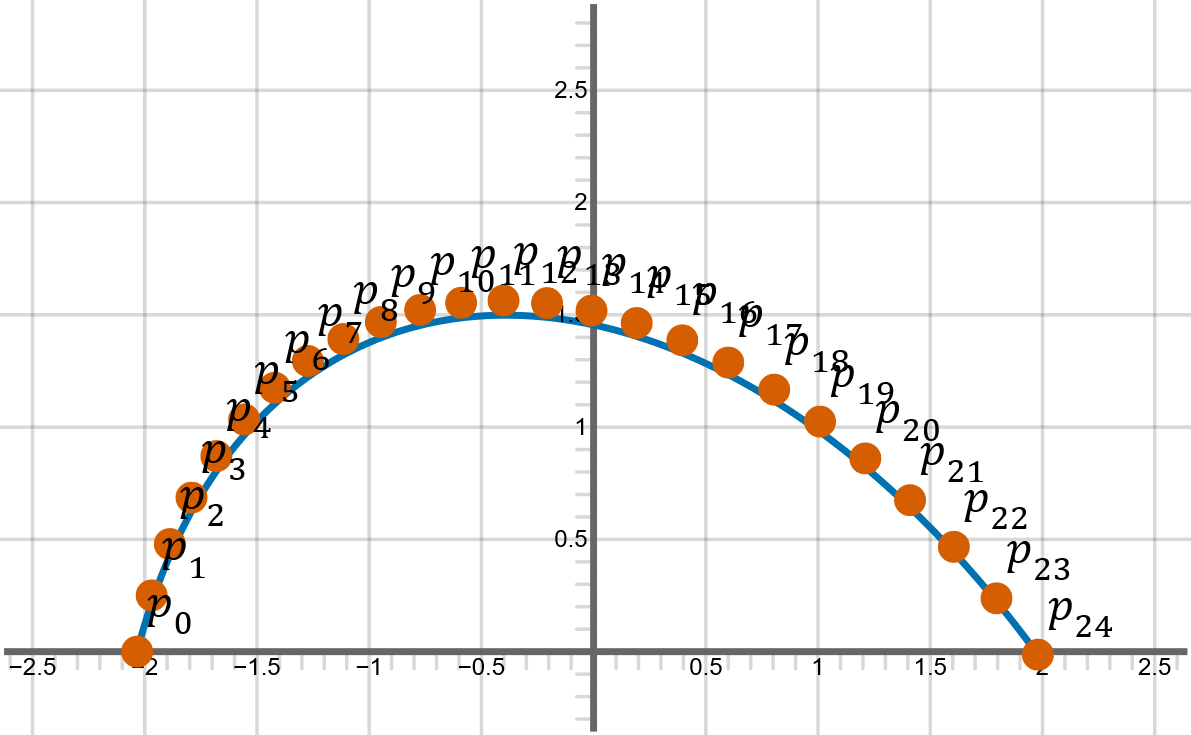
\includegraphics[width = \groupimagewidth]{images/dvig-n2}}
        \caption{Višanje stopnje Bézierjeve krivulje.}
        \label{fig:višanje}
    \end{figure}

    \subsection{Odvodi Bézierjeve krivulje}
    V kasnejših razdelkih bomo potrebovali odvode Bézierjevih krivulj, zato jih na tem mestu izpeljimo.
    Z upoštevanjem izreka~\ref{izrek:bernstein-odvod} o odvodu Bernsteinovih baznih polinomov dobimo
    \begin{align*}
        \mathbf{B}'(t) &=   &  &  &\left(\sum_{i=0}^{n}\p_{i}B_i^n(t)\right)' & & & =n \sum_{i=0}^{n}\p_{i}\left(B_{i-1}^{n-1}(t) - B_i^{n-1}(t)\right) \\
        &=            &  & &n \left( \sum_{i=1}^{n}\p_{i}B_{i-1}^{n-1}(t) - \sum_{i=0}^{n-1}\p_{i}B_i^{n-1}(t)\right) & & &= n \sum_{i=0}^{n-1}(\p_{i+1}-\p_{i})B_i^{n-1}(t).
    \end{align*}
    Za krajše zapise višjih odvodov Bézierjeve krivulje bomo uvedli operator  \textit{prema diferenca}, ki ga označimo z $\Delta$.
    Operator deluje na točki $\p_i$, definiramo pa ga rekurzivno kot
    \[\Delta^0\p_i=\p_i,\quad  \Delta^1\p_i= \Delta\p_i=\p_{i+1}-\p_{i}, \quad \Delta^k\p_i=\Delta^{k-1}\p_{i+1}-\Delta^{k-1}\p_{i}.\]
    Za naravno število $k$ lahko v zaključeni obliki podamo ekvivalenten zapis
    \[ \Delta^k\p_i= \sum_{j=0}^k\binom{k}{j}(-1)^{k-j}\p_{i+j}.\]
    \begin{opomba}
        Iz definicije je očitno, da je operator $\Delta^k$ definiran le na kontrolnih točkah z indeksi manjšimi ali enakimi $n-k$.
    \end{opomba}
    \noindent Odvode Bézierjeve krivulje lahko sedaj predstavimo s pomočjo preme diference.
    \begin{izrek}
        \label{izrek:odvod}
        Naj bo $\mathbf{B}$ Bézierjeva krivulja s kontrolnimi točkami $\p_i$, $i=0,1,\ldots,n$.
        Za njene odvode velja
        \[ \mathbf{B}^{(k)}(t) = \frac{n!}{(n-k)!} \sum_{i=0}^{n-k}\Delta^{k}\p_{i}B_i^{n-k}(t),\quad k=0,1,\ldots,n.\]
    \end{izrek}
    \noindent Izrek je enostavno dokazati s pomočjo indukcije, zato bomo dokaz izpustili.


    \section{Racionalne Bézierjeve krivulje}
    Pogosto s polinomskimi Bézierjevimi krivuljami ne moremo dovolj dobro (ali eksaktno) predstaviti določenih praktično uporabnih krivulj.
    Med njimi so tudi takšne, ki so za CAGD sisteme zelo pomembne, na primer krožni loki.
    Za opis takšnih krivulj lahko posežemo po racionalnih Bézierjevih krivuljah.
    Racionalno Bézierjevo krivuljo stopnje $n$ v $\R^d$ dobimo tako, da Bézierjevo krivuljo stopnje $n$ v $\R^{d+1}$ projiciramo na hiperravnino $w=1$.
    Točke iz $\R^{d+1}$ pri tem definiramo kot $(w,x_1,\ldots,x_n)$, projekcijo pa s predpisom $(w,\mathbf{x})\to(1,\frac{\mathbf{x}}{w})$.
    Takšna izpeljava privede do naslednje definicije.
    \begin{definicija}
        \label{def:racionalna}
        Racionalna Bézierjeva krivulja stopnje $n\in\N$ je racionalna krivulja podana s kontrolnimi točkami $\p_i\in\R^d$ in \textit{utežmi} $w_i\in\R$, $i=0,1,\ldots,n$, ter parametrizacijo $\mathbf{R}:[0,1]\to \R^d$  določeno s predpisom \[\mathbf{R}(t) = \frac{\sum^{n}_{i=0}w_i\p_i B^n_i(t)}{\sum^{n}_{i=0}w_i B^n_i(t)}.\]
    \end{definicija}
    \noindent Uteži so prosti parametri, ki jih lahko uporabimo pri oblikovanju.
    Kadar so vse uteži enake, je racionalna Bézierjeva krivulja polinomska Bézierjeva krivulja z istimi kontrolnimi točkami.
    Da bi se izognili težavam pri deljenju z $0$, ponavadi privzamemo, da so vse uteži pozitivne.
    Vpliv uteži si poglejmo na sliki~\ref{fig:uteži}.
    Utež spreminjamo le pri kontrolni točki $\p_1$, vse ostale uteži puščamo enake $1$.
    Na grafu (a) je utež nastavljena na število $1$, krivulja na sliki je zato polinomska Bézierjeva krivulja.
    Na grafih (b) in (c) lahko vidimo, da se z višanjem uteži, krivulja bliža točki $\p_1$.
    Na grafu (c) pa lahko vidimo, da se z nižanjem uteži, krivulja od točke $\p_1$ oddaljuje.
    \begin{figure}[h]
        \centering
        \subfloat[]{\includegraphics[width = \groupimagewidth]{images/racionalnaw1}}
        \qquad
        \subfloat[]{\includegraphics[width = \groupimagewidth]{images/racionalnaw2}}\\
        \subfloat[]{\includegraphics[width = \groupimagewidth]{images/racionalnaw4}}
        \qquad
        \subfloat[]{\includegraphics[width = \groupimagewidth]{images/racionalnaw05}}
        \caption{Vpliv uteži na racionalno Bézierjevo krivuljo.}
        \label{fig:uteži}
    \end{figure}

    Iz zapisa parametrizacije v definiciji~\ref{def:racionalna} lahko hitro vidimo, da množenje vseh uteži s poljubnim neničelnim številom krivulje ne spremeni.
    Tako lahko brez izgube splošnosti poljubno utež fiksiramo na $1$.
    Naslednji izrek pa pove, da lahko to storimo za dve uteži.
    \begin{izrek}
        \label{izrek:racionalne-utezi-1}
        Racionalno Bézierjevo krivuljo s pozitivnimi utežmi $w_i$ in parametrizacijo $\mathbf{R}$ lahko reparametriziramo v $\mathbf{\tilde{R}}$ s pozitivnimi utežmi $\tilde{w}_i$ tako, da velja $\tilde{w}_0=\tilde{w}_{n}=1.$
    \end{izrek}
    \noindent Dokaz izreka bo konstrukcijske narave.
    Našli bomo torej uteži $\tilde{w}_i$, katere lahko zamenjamo z utežmi $w_i$ tako, da ohranimo isto krivuljo.
    \begin{dokaz}
        Naj bo $\mathbf{R}$ racionalna Bézierjeva funkcija s poljubnimi pozitivnimi utežmi.
        Uporabimo reparametrizacijsko funkcijo $\varphi(t):[0,1]\to[0,1]$ s predpisom $\varphi(t)=\frac{t}{\rho(1-t)+t}$, kjer je $\rho$ pozitivno realno število.
        Če reparametrizacijsko funkcijo vstavimo v $i$-ti Bernsteinov bazni polinom dobimo
        \begin{align*}
            B^n_i(\varphi(t)) &=  \binom{n}{i}\left(\frac{t}{\rho (1-t)+t}\right)^i\left(1-\frac{t}{\rho (1-t)+t}\right)^{n-i} \\
            &=  \binom{n}{i}\left(\frac{t}{\rho (1-t)+t}\right)^i\left(\frac{\rho(1-t)}{\rho (1-t)+t}\right)^{n-i} \\
            &= \binom{n}{i}\frac{\rho^{n-1}t^{i}(1-t)^{n-i}}{(\rho(1-t)+t)^n} =  \frac{\rho^{n-1}}{(\rho(1-t)+t)^n}B^n_i(t).
        \end{align*}
        Reparametrizirane Bernsteinove bazne polinome sedaj vstavimo v parametrizacijo racionalne Bézierjeve krivulje, da dobimo
        \[\mathbf{\tilde{R}}(t)=\mathbf{R}(\varphi(t)) = \frac{\sum^{n}_{i=0}\rho^{n-i}w_i\p_i B^n_i(t)}{\sum^{n}_{i=0}\rho^{n-i}w_i B^n_i(t)}. \]
        Nove uteži izrazimo s starimi $\hat{w}_i=\rho^{n-i}w_i$.
        Želimo, da bi veljalo $\hat{w}_0=\hat{w}_n$, zato nastavimo $\rho= \sqrt[n]{\frac{w_n}{w_0}}$.
        Ker velja $\hat{w}_n=w_n$ lahko uteži $\hat{w}_i$ delimo z utežjo $w_n$, da dobimo željene uteži \[\tilde{w_i}=\frac{1}{w_n}\hat{w_i} = \frac{w_i}{\sqrt[n]{w^{i}_nw_0^{n-i}}}.\]
    \end{dokaz}
    \begin{posledica}
        Z uvedbo racionalnih Bézierjevih krivulj smo dobili le $n-1$ dodatnih prostih parametrov, glede na polinomske Bézierjeve krivulje z istim številom kontrolnih točk.
    \end{posledica}
    \begin{opomba}
        Če velja $w_0=w_n=1$ pravimo, da je racionalna Bézierjeva krivulja predstavljena v \textit{standardni obliki}.
    \end{opomba}
    Brez dokaza povejmo, da lastnosti Bézierjevih krivulj, ki smo jih podali v izreku~\ref{izrek:lastnosti-bezierjevih-krivulj}, veljajo tudi za racionalne Bézierjeve krivulje s pozitivnimi utežmi.
    Subdiviziranje, ekstrapoliranje in višanje stopnje polinomske Bézierjeve krivulje lahko na racionalne Bézierjeve krivulje stopnje $d$ razširimo tako, da krivuljo zapišemo kot polinomsko Bézierjevo krivuljo stopnje $d+1$ s kontrolnimi točkami  $(w_i,w_{i}\p_i)\in \R^{d+1}$.
    Polinomsko krivuljo nato subdiviziramo/ekstrapoliramo/ji zvišamo stopnjo in iz dobljenih kontrolnih točk $(\tilde{w}_i,\tilde{w}_{i}\tilde{\p}_i)\in\R^{d+1}$ preberemo nove kontrolne točke $\tilde{\p_i}\in\R^d$ in uteži $\tilde{w_i}\in\R$.
    Pri takšnem procesu samo ekstrapolacija ne ohranja pozitivnosti uteži.
    Primere si lahko ogledamo na sliki~\ref{fig:razsirjene-metode}.
    \begin{figure}[h]
        \captionsetup[subfigure]{labelformat=empty}
        \centering
        \subfloat[začetna krivulja]{\includegraphics[width = \groupimagewidth]{images/racionalna-start}}
        \qquad
        \subfloat[subdivizija]{\includegraphics[width = \groupimagewidth]{images/racionalna-subdivizija}}\\
        \subfloat[ekstrapolacija]{\includegraphics[width = \groupimagewidth]{images/racionalna-ekstrapolirana}}
        \qquad
        \subfloat[višanje stopnje]{\includegraphics[width = \groupimagewidth]{images/racionalna-dvig}}
        \caption{Subdivizija, ekstrapolacija ter višanje stopnje racionalne Bézierjeve krivulje z utežmi $w_1=2$, $w_0=w_2=w_3=1$.}
        \label{fig:razsirjene-metode}
    \end{figure}
%    Interpolacijo točk lahko dokažemo na podoben način, kakor smo to storili pri dokazu izreka~\ref{izrek:lastnosti-bezierjevih-krivulj}.
%    Da dokažemo, da je racionalna Bézierjeva krivulja afino invariantna, ter da leži znotraj konveksne ovojnice kontrolnih točk, pa posežemo po naslednjem zapisu.
%    \[\mathbf{R}(t)=\sum^n_{i=0}\p_i N^n_i, \quad N^n_i(t)\coloneqq \frac{w_i B^n_i(t)}{\sum^n_{i=0}w_i B^n_i(t)}\]
%    Če pri dokazu izreka~\ref{izrek:lastnosti-bezierjevih-krivulj} namesto Bernsteinovih polinomov $B_i^n(t)$ vstavimo funkcijo $N^n_i$ iz zgornjega zapisa, dobimo dokaz lastnosti za racionalne Bézierjeve krivulje.

    \subsection{De Casteljaujev algoritem za racionalne Bézierjeve krivulje}
    Točke racionalnih Bézierjevih krivulj dimenzije $d$ bi lahko računali s pomočjo de Casteljaujevega algoritma za polinomske Bézierjeve krivulje stopnje $d+1$ na podoben način, kot smo v prejšnjem razdelku razširili subdivizijo, ekstrapolacijo in višanje stopnje krivulje.
    Takšno računanje točk se izkaže za nestabilno~\cite{stability-rational}, zato na tem mestu podamo algoritem~\ref{alg:racionalni-decasteljau}, ki je razširitev de Casteljaujevega algoritma za racionalne Bézierjeve krivulje in točke racionalne Bézierjeve krivulje računa stabilno.
    \begin{algorithm}[h!]
        \caption{Racionalni de Casteljaujev algoritem}
        \begin{algorithmic}
            \State $\p \gets \p_0,\p_1,\dots,\p_n$
            \State $w\gets w_0,w_1,\dots,w_n$
            \For{$i = 0,1,\dots n$}
                \State $\p_i^0(t)=\p_i$
                \State $w_i^0(t)=w_i$
            \EndFor
            \For{$r = 1,2,\dots n$}
                \For{$i=0,1,\dots,n-r$}
                    \State $w_i^r(t)=(1-t)w_{i}^{r-1}(t)+tw_{i+1}^{r-1}(t)$
                    \State $\p_i^r(t)=(1-t)\frac{w_{i}^{r-1}(t)}{w_{i}^{r}(t)}\p_i^{r-1}(t)+t\frac{w_{i+1}^{r-1}(t)}{w_{i}^{r}(t)}\p_{i+1}^{r-1}(t)$
                \EndFor
            \EndFor
            \State \Return $\p_0^n(t)$
        \end{algorithmic}\label{alg:racionalni-decasteljau}
    \end{algorithm}
    \noindent Brez dokaza z naslednjim izrekom podajmo pravilnost algoritma~\ref{alg:racionalni-decasteljau}.
    \begin{izrek}
        Naj bo $t\in\R$ in $\p_i^r(t)$ vmesne točke iz algoritma~\ref{alg:racionalni-decasteljau}.
        Potem je
        \[\p_i^r(t)= \frac{\sum^{r}_{j=0}w_{i+j}\p_{i+j} B^r_j(t)}{\sum^{n}_{i=0}w_{i+j} B^r_j(t)}. \]
    \end{izrek}

    \subsection{Farinove točke}
    Uporabniku CAGD sistema želimo nuditi čim bolj naraven način kontroliranja uteži racionalne Bézierjeve krivulje.
    V ta namen lahko uteži predstavimo s \textit{Farinovimi točkami}.
    Farinove točke ležijo na daljicah kontrolnega poligona, kjer $i$-ta Farinova točka $\mathbf{f}_i$ deli $i$-to daljico kontrolnega poligona v razmerju $w_{i+1}:w_{i}$.
    Slednje lahko zapišemo kot \[\frac{||\mathbf{f}_i-\p_i||}{||\mathbf{f}_i-\p_{i+1}||} = \frac{w_{i+1}}{w_{i}}.\]
    S kontrolnimi točkami in utežmi lahko Farinove točke izrazimo kot
    \[\mathbf{f}_i \coloneqq \frac{w_{i}}{w_{i}+w_{i+1}}\p_i +  \frac{w_{i+1}}{w_{i}+w_{i+1}}\p_{i+1}.\]
    Da bi uporabnik lahko s Farinovimi točkami kontroliral uteži, želimo s Farinovimi točkami izraziti uteži.
    Brez izgube splošnosti lahko za prvo utež izberemo $w_0=1$.
    Ostale točke lahko nato rekurzivno izračunamo s pomočjo izraza
    \[w_{i+1} = w_i\frac{||\mathbf{f}_i-\p_i||}{||\mathbf{f}_i-\p_{i+1}||}.\]
    Po želji lahko uteži tudi standardiziramo s pomočjo formule \[\tilde{w}_{i} = \frac{w_i}{\sqrt[n]{w_n^i}},\]
    ki sledi iz dokaza izreka~\ref{izrek:racionalne-utezi-1}.

    Na sliki~\ref{fig:farinove-tocke} si lahko ogledamo delovanje Farinovih točk.
    Uteži na sliki niso standardizirane zato, da lahko bolje vidimo razmerja med njimi.
    Na grafu (a) Farinove točke ležijo na sredini pripadajočih daljic.
    Posledično so vsa razmerja $||\p_i-\mathbf{f}_i||:||\p_{i+1}-\mathbf{f}_i||$ enaka in vse uteži enake $1$.
    Na grafu (b) lahko vidimo, da se s premikom prve Farinove točke bližje k točki $\p_0$, k njej približa tudi krivulja.
    Utež $w_1$, ki predstavlja razmerje $||\p_0-\mathbf{f}_0||:||\p_{1}-\mathbf{f}_0||$, je zato manjša kot $1$.
    Na grafu (c) lahko vidimo premik Farinove točke bližje k točki $\p_1$.
    Krivulja se točki približa, utež $w_1$ pa se poveča na več kot $1$.
    Ker na grafih (b) in (c) druga in tretja Farinova točka ležita na sredini ustreznih daljic, so uteži $w_1$,$w_2$ in $w_3$ enake.
    Na grafih (d) in (e) lahko vidimo, kako se krivulja in uteži obnašajo ob premiku druge Farinove točke.
    Na grafih (f) ter (g) pa lahko vidimo obnašanje krivulje, ko premaknemo prvo ter tretjo Farinovo točko hkrati višje oziroma nižje.
    Poglejmo še, kaj se zgodi, če vse tri točke premaknemo pomaknemo tako, da so razmerja na vseh daljicah enaka.
    Na levem grafu slike~\ref{fig:farinove-tocke-2} lahko vidimo, da krivulja izgleda kakor začetna.
    Če uteži standardiziramo, kar smo storili na desnem grafu, vidimo, da je temu res tako.
    Da bi preprečili takšno izbiro Farinovih točk, lahko po vsakem premiku Farinove točke uteži standardiziramo, ter ponovno izračunamo Farinove točke.
    \begin{figure}[h!]
        \centering
        \subfloat[]{\includegraphics[width = \groupimagewidth]{images/farinove-tocke-premik-0}}\\
        \subfloat[]{\includegraphics[width = \groupimagewidth]{images/farinove-tocke-premik-leva-1}}
        \qquad
        \subfloat[]{\includegraphics[width = \groupimagewidth]{images/farinove-tocke-premik-leva-2}}
        \qquad
        \subfloat[]{\includegraphics[width = \groupimagewidth]{images/farinove-tocke-premik-zgornja-1}}
        \qquad
        \subfloat[]{\includegraphics[width = \groupimagewidth]{images/farinove-tocke-premik-zgornja-2}}
        \qquad
        \subfloat[]{\includegraphics[width = \groupimagewidth]{images/farinove-tocke-premik-obe-1}}
        \qquad
        \subfloat[]{\includegraphics[width = \groupimagewidth]{images/farinove-tocke-premik-obe-2}}
        \caption{Kontroliranje krivulje s Farinovimi točkami.}
        \label{fig:farinove-tocke}
    \end{figure}

    \begin{figure}[h!]
        \centering
        \subfloat[]{\includegraphics[width = \groupimagewidth]{images/farinove-tocke-premik-vsetri-0}}
        \qquad
        \subfloat[]{\includegraphics[width = \groupimagewidth]{images/farinove-tocke-premik-vsetri-1}}
        \caption{Krivulja z enakimi premiki vseh Farinovih točk, pred in po standardizaciji.}
        \label{fig:farinove-tocke-2}
    \end{figure}

%    \subsubsection{Izsek krožnice}
%    V uvodu podrazdelka smo povedali, da se nekaterih krivulj ne da opisati z navadnimi Bézierjevimi krivuljami.
%    Kot enega izmed primerov smo podali izsek krožnice.
%    V tem delu podrazdelka bomo izpeljali kontrolne točke in uteži racionalne Bézierjeve krivulje, da bo krivulja predstavljala izsek krožnice s polmerom $R$ in \mycomment{kotom $\alpha$}.
%    Izsek krožnice bomo podali s kvadratičnimi racionalnimi Bézierjevimi krivuljami.
%    Za konstrukcijo imamo na voljo kontrolne točke $\p_0,\p_1$ in $\p_2$, ter uteži $w_0,w_1$ in $w_2$.
%    Iz izreka~\ref{izrek:racionalne-utezi-1} sledi, da lahko robni uteži fiksiramo na $w_0=w_2=1$.
%    Točki $\p_0$ in $\p_2$ morata ležati na začetku ter koncu izseka krožnice, saj racionalne Bézierjeve krivulje interpolirajo končne točke.
%    Ker so racionalne Bézierjeve krivulje afino invariantne, lahko brez izgube splošnosti postavimo točki $\p_0$ in $\p_2$ tako, da velja $\p_0=-\p_2$.
%    Parametrizacija željene krivulje izgleda takole
%    \[\mathbf{R}(t) = \frac{\sum^{2}_{i=0}w_i\p_i B^2_i(t)}{\sum^{2}_{i=0}w_i B^2_i(t)} = \frac{\p_0 (1-t)^2 + w_1\p_1 2t(1-t) + \p_2 t^2}{(1-t)^2 + w_1 2t(1-t) + t^2}.\]
%    Velja torej $T=R(\frac{1}{2})= \frac{w_1\p_1}{w_1+1}$.
%    Poglejmo si sliko\mycomment{referenca}.
%    Iz nje lahko razberemo zvezi
%    \begin{align*}
%        ||OT||=||ST||-||SO|| = R - R\sin\frac{\alpha}{2} = R(1-\sin\frac{\alpha}{2})\\
%        ||O\p_1|| = ||S\p_1||-||SO|| = \frac{R}{\sin\frac{\alpha}{2}} - R\sin\frac{\alpha}{2} = R\frac{1-\sin^2\frac{\alpha}{2}}{\sin\frac{\alpha}{2}}
%    \end{align*}
%    Iz zveze $\frac{||OT||}{||O\p_1||} = \frac{\sin\frac{\alpha}{2}}{\sin\frac{\alpha}{2}+1} = \frac{w_1}{w_1+1}$ nato sledi $w_1=\sin\frac{\alpha}{2}$.
%    Pričakujemo, da bo točka $\p_1$ oblike $(0,y)$.
%    Velja torej $||O\p_1||=y=R\frac{1-\sin^2\frac{\alpha}{2}}{\sin\frac{\alpha}{2}}$.
%
%%
%%
%%%    po komponentah pa
%%%    \begin{align*}
%%%        x(t) &= \frac{(1-t)^2 + w_1R\cos\left(\frac{\alpha}{2}\right) 2t(1-t) + \cos(\alpha)t^2}{(1-t)^2 + w_1 2t(1-t) + t^2} \\
%%%        y(t) &= \frac{w_12t(1-t)R\sin\left(\frac{\alpha}{2}\right) + \sin(\alpha)t^2}{(1-t)^2 + w_1 2t(1-t) + t^2}.
%%%    \end{align*}
%%    Tangenta na enotsko krožnico je v točki $(1,0)$ vzporedna z ordinatno osjo, zato mora veljati $x'(0)=0$.
%%    \mycomment{Odvod racionalne Bézierjeve krivulje v točki $(1,0)$ je enak $2(\p_{1}-\p_{0}) = 2\left(R\sin\left(\frac{\alpha}{2}\right)-r,R\cos\left(\frac{\alpha}{2}\right)\right)$.}
%%    Iz česar sledi $R=\frac{r}{\cos\left(\frac{\alpha}{2}\right)}$.
%%    \begin{align*}
%%        w_1\left(\frac{r}{\sin\left(\frac{\alpha}{2}\right)}-r\right)\sin\left(\frac{\alpha}{2}\right)  &= r\sin\left(\frac{\alpha}{2}\right) - \frac{r}{2}\sin(\alpha) \\
%%        w_1 &= \frac{r\sin\left(\frac{\alpha}{2}\right) - \frac{r}{2}\sin(\alpha)}{\left(\frac{r}{\sin\left(\frac{\alpha}{2}\right)}-r\right)\sin\left(\frac{\alpha}{2}\right) }
%%    \end{align*}
%%
%%
%%    Zaradi simetrije mora krivulja v $t=\frac{1}{2}$ interpolirati točko $\left(\cos\left(\frac{\alpha}{2}\right),\sin\left(\frac{\alpha}{2}\right)\right)$ iz česar sledi
%%    \begin{align*}
%%        x\left(\frac{1}{2}\right) &= \frac{\frac{1}{4} +  \frac{1}{2}w_1R\cos\left(\frac{\alpha}{2}\right) + \frac{1}{4}\cos(\alpha)}{\frac{1}{4}+ w_1\frac{1}{2} + \frac{1}{4}} = \frac{ \frac{1}{2} + w_1R\cos\left(\frac{\alpha}{2}\right) + \frac{1}{2}\cos(\alpha)}{1+w_1} = \cos\left(\frac{\alpha}{2}\right) \\
%%        y\left(\frac{1}{2}\right) &= \frac{\frac{w_1}{2}R\sin\left(\frac{\alpha}{2}\right) + \frac{1}{4}\sin(\alpha)}{\frac{1}{4}+ w_1\frac{1}{2} + \frac{1}{4}} =  \frac{w_1R\sin\left(\frac{\alpha}{2}\right) + \frac{1}{2}\sin(\alpha)}{1+w_1} = \sin\left(\frac{\alpha}{2}\right).
%%    \end{align*}
%%    Iz enačbe izpostavimo $w_1$
%%    \begin{align*}
%%        \frac{1}{2} + w_1R\cos\left(\frac{\alpha}{2}\right) + \frac{1}{2}\cos(\alpha) &= (1+w_1)\cos\left(\frac{\alpha}{2}\right) \\
%%        w_1R\cos\left(\frac{\alpha}{2}\right) - w_1\cos\left(\frac{\alpha}{2}\right) &= \cos\left(\frac{\alpha}{2}\right)-\frac{1}{2} - \frac{1}{2}\cos(\alpha) \\
%%        w_1(R-1)\cos\left(\frac{\alpha}{2}\right) &= \left(\cos\left(\frac{\alpha}{2}\right)-\frac{1}{2} - \frac{1}{2}\cos(\alpha)\right)
%%    \end{align*}
%%    NEXT
%%    \begin{align*}
%%        w_1R\sin\left(\frac{\alpha}{2}\right) + \frac{1}{2}\sin(\alpha) &= (1+w_1)\sin\left(\frac{\alpha}{2}\right) \\
%%        w_1(R-1)\sin\left(\frac{\alpha}{2}\right)  &= \sin\left(\frac{\alpha}{2}\right) - \frac{1}{2}\sin(\alpha)
%%    \end{align*}
%%
%%    \begin{align*}
%%        \frac{r}{2} + w_1R\cos\left(\frac{\alpha}{2}\right) + \frac{r}{2}\cos(\alpha) &=(1+w_1) r\cos\left(\frac{\alpha}{2}\right) \\
%%        w_1R\cos\left(\frac{\alpha}{2}\right) - w_1r\cos\left(\frac{\alpha}{2}\right) &= r\cos\left(\frac{\alpha}{2}\right)-\frac{r}{2}\cos(\alpha)-\frac{r}{2} \\
%%        w_1(R-r)\cos\left(\frac{\alpha}{2}\right) &= r\cos\left(\frac{\alpha}{2}\right)-\frac{r}{2}\cos(\alpha)-\frac{r}{2} \\
%%        w_1 &=\frac{r\cos\left(\frac{\alpha}{2}\right)-\frac{r}{2}\cos(\alpha)-\frac{r}{2}}{(R-r)\cos\left(\frac{\alpha}{2}\right)}\\
%%        w_1 &=\frac{r\cos\left(\frac{\alpha}{2}\right)-\frac{r}{2}\cos(\alpha)-\frac{r}{2}}{(R=\frac{r}{\cos\left(\frac{\alpha}{2}\right)}-r)\cos\left(\frac{\alpha}{2}\right)}
%%    \end{align*}
%%
%%
%%
%%    \begin{align*}
%%        w_1\left(\frac{r}{\sin\left(\frac{\alpha}{2}\right)}-r\right)\sin\left(\frac{\alpha}{2}\right)  &= r\sin\left(\frac{\alpha}{2}\right) - \frac{r}{2}\sin(\alpha) \\
%%        w_1 &= \frac{r\sin\left(\frac{\alpha}{2}\right) - \frac{r}{2}\sin(\alpha)}{\left(\frac{r}{\sin\left(\frac{\alpha}{2}\right)}-r\right)\sin\left(\frac{\alpha}{2}\right) }
%%    \end{align*}
%%    Izračunajmo sedaj za $r=1$ in $\alpha = \frac{\pi}{2}$. $R=\frac{1}{\cos\left(\frac{\pi}{4}\right)} = \sqrt{2}.$
%%    \[ w_1 = \frac{\frac{\sqrt{2}-1}{2}}{(\sqrt{2}-1)\frac{\sqrt{2}}{2}} = \frac{\sqrt{2}-1}{(\sqrt{2}-1)\sqrt{2}} = \frac{\sqrt{2}}{2} \]
%
    \clearpage


    \section{Zlepki Bézierjevih krivulj}
    Če si ponovno ogledamo de Casteljaujev algoritem~\ref{alg:decasteljau}, lahko hitro opazimo, da je časovna kompleksnost algoritma $O(n^2)$.
    Računanje točk kompleksnejše Bézierjeve krivulje, z veliko kontrolnimi točkami,  je zato zamudno.
    Da bi ohranili uporabniku naravno kontrolo krivulj ter hiter izračun točk, posežemo po zlepkih Bézierjevih krivulj.
    \begin{definicija}
        Zlepek krivulj $\mathbf{S}:[a,b]\to \R^d$ nad zaporedjem stičnih točk \[a=u_0 < u_1 < \cdots < u_{m-1} < u_m = b\] je parametrično podana polinomska krivulja stopnje $n\in\N$, katere komponente so odsekoma polinomske funkcije $\mathbf{S}|_{[u_{l-1},u_l]} \in \Pn^d$, $l=1,2\ldots,m$.
    \end{definicija}
    \noindent Želimo, da bi zlepki tvorili gladko neprekinjeno krivuljo, saj so takšne krivulje v CAGD sistemih najbolj uporabne.
    Krivulja je po definiciji na posameznih odsekih polinomska in zato tudi gladka, problem je le v stičnih točkah.
    Naj bo
    \begin{align}
        \mathbf{S}(u) = \begin{dcases}
                            \mathbf{S}_1(u) = \sum_{i=0}^n \p_i^{(1)}B_i^n\left(\frac{u-u_0}{\Delta u_0}\right), & u \in [u_0,u_1),  \\
                            \mathbf{S}_2(u) = \sum_{i=0}^n \p_i^{(2)}B_i^n\left(\frac{u-u_1}{\Delta u_1}\right), & u \in [u_1,u_2],
        \end{dcases} \label{eq:zlepek-def}
    \end{align}
    zlepek dveh Bézierjevih krivulj.
    Da bo zlepek zvezen, mora v stični točki $u_1$ veljati $\mathbf{S}_1(u_1) = \mathbf{S}_2(u_1)$ oziroma
    \begin{align}
        \label{c0-zlepek-ref}
        \p_n^{(1)} = \p_0^{(2)}.
    \end{align}
    Takšen zlepek, si lahko ogledamo na sliki~\ref{fig:zlepek-c0}.
    \begin{figure}[h]
        \centering
        \includegraphics[width = 0.50\textwidth]{images/zlepek-c0}
        \caption{$C^0$ zlepek dveh Bézierjevih krivulj.}
        \label{fig:zlepek-c0}
    \end{figure}

    \noindent Da bo zlepek vsaj zvezno odvedljiv, mora veljati~\eqref{c0-zlepek-ref}, morata pa v stični točki sovpadati tudi odvoda $\mathbf{S}_1'(u_1) = \mathbf{S}_2'(u_1)$.
    Iz izreka~\ref{izrek:odvod} sledi, da mora zato veljati
    \begin{align}
        \frac{\p_{n}^{(1)} - \p_{n-1}^{(1)}}{\Delta u_0} = \frac{\p_{1}^{(2)} - \p_{0}^{(2)}}{\Delta u_1}.
    \end{align}
    Upoštevajoč~\eqref{c0-zlepek-ref} lahko enačbo zapišemo tudi kot
    $$\p_{n}^{(1)} =  \p_{0}^{(2)}  = \frac{\Delta u_0\p_{1}^{(2)}}{\Delta u_0+\Delta u_1} + \frac{\Delta u_1\p_{n-1}^{(1)}}{\Delta u_0+\Delta u_1} ,$$
    od koder je moč prebrati geometrijski pomen pogoja.
    Skupna točka $\p_{n}^{(1)} =  \p_{0}^{(2)}$ mora namreč deliti daljico $\p_{n-1}^{(1)}\p_{1}^{(2)}$ v razmerju $\frac{\Delta u_0}{\Delta u_1}$.
    Primer takšnega zlepka si lahko ogledamo na sliki~\ref{fig:zlepek-c1}.
    \begin{figure}[h]
        \centering
        \includegraphics[width = 0.50\textwidth]{images/zlepek-c1}
        \caption{$C^1$ zlepek dveh Bézierjevih krivulj, kjer je $\Delta u_0=\Delta u_1$.}
        \label{fig:zlepek-c1}
    \end{figure}
    Podobno lahko iz izreka~\ref{izrek:odvod} preberemo pogoje gladkosti za $C^r([a,b])$,
    $$ \frac{1}{(\Delta u_0)^k}\Delta^k\p^{(1)}_{n-k}= \frac{1}{(\Delta u_1)^k}\Delta^k\p^{(2)}_{0}, \quad k=0,\dots,r.$$
    Primer $C^2$ oziroma $C^3$ zlepka si lahko ogledamo na sliki~\ref{fig:zlepek-c2} oziroma sliki~\ref{fig:zlepek-c3}.
    \begin{figure}[h]
        \centering
        \includegraphics[width = 0.50\textwidth]{images/zlepek-c2}
        \caption{$C^2$ zlepek dveh Bézierjevih krivulj, kjer je $\Delta u_0=\Delta u_1$.}
        \label{fig:zlepek-c2}
    \end{figure}
    \begin{figure}[h]
        \centering
        \includegraphics[width = 0.50\textwidth]{images/zlepek-c3}
        \caption{$C^3$ zlepek dveh Bézierjevih krivulj, kjer je $\Delta u_0=\Delta u_1$.}
        \label{fig:zlepek-c3}
    \end{figure}

    \subsection{Geometrijska zveznost}
    Da bi zlepki bili gladki, ne potrebujemo zvezne odvedljivosti v analitičnem smislu, dovolj je zvezna odvedljivost v geometrijskem smislu.
    \begin{definicija}
        \label{def:geometrijska-zveznost}
        Zlepek krivulj \[\mathbf{S}(u) = \begin{cases}
                                             \mathbf{S}_1(u), & u \in [u_0,u_1),  \\
                                             \mathbf{S}_2(u), & u \in [u_1,u_2],
        \end{cases}\] je $k$-krat geometrijsko zvezno odvedljiv ($G^k$), če v okolici stične točke $u_1$ obstaja takšna regularna reparametrizacijska funkcija $\varphi$, da je $\varphi(u_1)=u_1$ in je zlepek krivulj
        \[\mathbf{S}(u) = \begin{cases}
                              \mathbf{S}_1(u), & u \in [u_0,u_1),  \\
                              \mathbf{S}_2(\varphi(u)), & u \in [u_1,u_2],
        \end{cases}\]
        $k$-krat zvezno odvedljiv.
    \end{definicija}
    \noindent Izpeljimo sedaj pogoje gladkosti za $G^k$, $k=0,1,2$.
    Za $G^0$ mora veljati
    \begin{align}
        \mathbf{S}_1(u_1) =  \mathbf{S}_2(\varphi(u_1))=  \mathbf{S}_2(u_1), \label{eq:g0-pogoj}
    \end{align}
    kar je enak pogoj kakor za $C^0$.
    Za $G^1$ mora veljati~\eqref{eq:g0-pogoj} in \begin{align}
                                                     \mathbf{S}_1'(u_1) = \mathbf{S}_2'(\varphi(u_1))\varphi'(u_1) = \mathbf{S}_2'(u_1)\varphi'(u_1). \label{eq:g1-pogoj-1}
    \end{align}
    Za $G^2$ pa mora veljati~\eqref{eq:g0-pogoj} in~\eqref{eq:g1-pogoj-1} ter \[\mathbf{S}_1''(u_1) = \mathbf{S}_2''(\varphi(u_1))(\varphi'(u_1))^2 +  \mathbf{S}_2'(\varphi(u_1))\varphi''(u_1) =\mathbf{S}_2''(u_1)(\varphi'(u_1))^2 +  \mathbf{S}_2'(u_1))\varphi''(u_1).\]
    Če sedaj označimo odvode reparametrizacijske funkcije v točki $u_1$ z $\beta_i = \varphi^{(i)}(u_1)$, lahko pogoje za $G^2$ zveznost izrazimo s povezovalno matriko
    \[
        \begin{bmatrix}
            \mathbf{S}_1'(u_1) \\
            \mathbf{S}_1''(u_1)
        \end{bmatrix}
        =
        \begin{bmatrix}
            \beta_1 & 0         \\
            \beta_2 & \beta_1^2
        \end{bmatrix}  \begin{bmatrix}
                           \mathbf{S}_2'(u_1) \\
                           \mathbf{S}_2''(u_1)
        \end{bmatrix}.\]
    Lahko pa tudi najprej izberemo pozitiven skalar $\beta_1$ in poljuben skalar $\beta_2$, ter konstruiramo reparametrizacijsko funkcijo, ki ustreza pogojem $\varphi'>0$,  $\varphi'(u_1)=\beta_1$ in $\varphi'(u_1)=\beta_2$.
    Za funkcijo $\varphi$ lahko vzamemo kar Taylorjev polinom
    \[\varphi(u) = u_1 + \beta_1(u-u_1) + \frac{1}{2}\beta_2(u-u_1)^2.\]

    Oglejmo si sedaj, kako pogoji za geometrijsko zveznost vplivajo na zlepke Bézierjevih krivulj.
    Da je zlepek~\eqref{eq:zlepek-def} $G^1$ zvezen, mora veljati  $\mathbf{S}_1'(u_1) = \beta_1\mathbf{S}_2'(u_1)$, iz česar sledi
    \[\frac{\p_{n}^{(1)} - \p_{n-1}^{(1)}}{\Delta u_0} = \beta_1\frac{\p_{1}^{(2)} - \p_{0}^{(2)}}{\Delta u_1}.\]
    Če označimo sedaj $\alpha_1=  \frac{\beta_1\Delta u_0}{\Delta u_1}$ lahko pogoj zapišemo kot
    \begin{align}
        \p_{n}^{(1)} - \p_{n-1}^{(1)}= \alpha_1(\p_{1}^{(2)} - \p_{0}^{(2)}).\label{eq:g1-pogoj}
    \end{align}
    Glede na $C^1$  smo torej pridobili prosti parameter, ki ga lahko v CAGD sistemih uporabimo za dodatno kontrolo nad krivuljo.
    Primer $G^1$ zlepka in vpliv izbire $\beta_1$ si lahko ogledamo na sliki~\ref{fig:zlepek-g1}.
    \begin{figure}[h]
        \captionsetup[subfigure]{labelformat=empty}
        \centering
        \subfloat[$\beta_1=1$]{\includegraphics[width = \groupimagewidth]{images/zlepek-g1}}
        \qquad
        \subfloat[$\beta_1<1$]{\includegraphics[width = \groupimagewidth]{images/zlepek-g1-2}}
        \qquad
        \subfloat[$\beta_1>1$]{\includegraphics[width = \groupimagewidth]{images/zlepek-g1-3}}
        \caption{Vpliv izbire $\beta_1$ pri $G^1$ zlepku.}
        \label{fig:zlepek-g1}
    \end{figure}

    \subsection{Konstrukcija zlepkov Bézierjevih krivulj}\label{subsec:konstrukcija-zlepkov}
%    V tem podrazdelku bomo podali nekaj algoritmov za konstrukcijo zlepkov Bézierjevih krivulj.
%    Najprej bomo predstavili enostransko konstrukcijo $C^r$ zlepka za poljuben $r$, ki bo bolj teoretične narave.
%    Nadaljevali pa bomo s simetričnimi konstrukcijami, ki so uporabne tudi v praksi.
%    Pri slikovnem gradivu, bomo fiskne točke iz algoritmov označevali z zeleno barvo.

    \subsubsection{Enostranska konstrukcija}
    Pogoje gladkosti iz prejšnjega razdelka bi lahko izpeljali tudi drugače.
    Da bi zlepek~\eqref{eq:zlepek-def} bil $C^{\infty}$, bi morali krivulji $\mathbf{S}_1$ in $\mathbf{S}_2$ biti del iste Bézierjeve krivulje.
    Krivuljo $\mathbf{S}_2$ lahko zato dobimo z ekstrapolacijo krivulje $\mathbf{S}_1$.
    Da je zlepek $C^r$ je dovolj, da krivulja $\mathbf{S}_2$ ustreza ekstrapolirani krivulji v prvih $r+1$ kontrolnih točkah, saj le te vplivajo na prvih $r$ odvodov krivulje $\mathbf{S}_2$ v stični točki $u_1$.
    Zlepek gladkosti $r$ lahko torej konstruiramo tako, da začnemo z Bézierjevo krivuljo.
    Krivuljo nato ekstrapoliramo in ekstrapoliranemu delu fiksiramo prvih $r+1$ točk, ostale pa izberemo poljubno.
    Postopek je podrobneje zapisan v algoritmu~\ref{alg:C-n}, kjer funkcija decasteljau\_shema predstavlja funkcijo, ki vrača De Casteljaujevo shemo~\ref{fig:decasteljau-scheme}.
    \begin{algorithm}[H]
        \caption{Enostranska konstrukcija $C^r$ zlepka stopnje $n$}
        \label{alg:C-n}
        \begin{algorithmic}
            \State Vhod:
            \State $\p \gets \p_0,\p_1,\dots,\p_{m}$
            \State $u \gets u_0,u_1,\dots,u_n$
            \State
            \State st\_krivulj = $\frac{m-n}{n-r}$
            \For{$i = 0,1,\dots n$}
                \State $\p_i^{(1)}=\p_i$
            \EndFor
            \For{$j = 2,3\dots$st\_krivulj}
                \State $t_0$ = $\frac{\Delta u_j + \Delta u_{j+1}}{\Delta u_j}$
                \State $\mathbf{e}$ = decasteljau\_shema($\p^{(j-1)}$, $t_0$)
                % return decasteljau[lenn - 1][lenn - j - 1].X();
                \State $\{\p_i^{(j)}\}_{i=0}^{r}$ = $\{\mathbf{e^{(n)}_{j}}\}_{j=n}^{n-r}$
                \For{$k = 0,1,\dots (n-r)$}
                    \State $\p_{n-r+k}^{(j)}=\p_{j(n-r)+k}$
                \EndFor
            \EndFor
            \State
            \State \Return $\{\mathbf{p^{(i)}}\}^{st\_krivulj}_{i=1}$
        \end{algorithmic}
    \end{algorithm}
    \noindent Zlepki, konstruirani s takšnim algoritmom, niso uporabniku prijazni, saj kontrolne točke različno vplivajo na obliko krivulje.
    Za primer si na sliki~\ref{fig:enostranski-c1} oglejmo obnašanje tako konstruiranega kvadratnega $C^1$ zlepka.
    \begin{figure}[h]
        \captionsetup[subfigure]{labelformat=empty}
        \centering
        \subfloat[začetni zlepek]{\includegraphics[width = \groupimagewidth]{images/enostranski-spline-1}}
        \qquad
        \subfloat[premik $\p_1$]{\includegraphics[width = \groupimagewidth]{images/enostranski-spline-3}}
        \qquad
        \subfloat[premik $\p_5$]{\includegraphics[width = \groupimagewidth]{images/enostranski-spline-2}}
        \caption{Obnašanje enostranskega kvadratnega $C^1$ zlepka.}
        \label{fig:enostranski-c1}
    \end{figure}

    \subsubsection{Simetrična konstrukcija}
    Uporabniku mnogo bolj prijazni so algoritmi simetričnih konstrukcij.
    Brez izpeljave podajmo algoritma~\ref{alg:C-1}~in~\ref{alg:C-2} za simetrični konstrukciji kvadratnega $C^1$ in kubičnega $C^2$ zlepka.
    Obnašanje tako konstruiranih zlepkov si lahko ogledamo na slikah~\ref{fig:simetricni-c1} in~\ref{fig:simetricni-c2}.
    \begin{algorithm}[H]
        \caption{Simetrična konstrukcija kvadratnega $C^1$ zlepka}
        \label{alg:C-1}
        \begin{algorithmic}
            \State Vhod:
            \State $\p \gets \p_0,\p_1,\dots,\p_{m+1}$
            \State $u \gets u_0,u_1,\dots,u_m$
            \State
            \State $\p_0^{(1)} = \p_0$
            \State $\p_1^{(1)} = \p_1$
            \For{$l = 1,2,\dots m-1$}
                \State $\p_1^{(l)}=\p_{l}$
                \State $\p_2^{(l)} = \p_0^{(l+1)} = \frac{\Delta u_l}{\Delta u_{l-1} + \Delta u_{l}}\p_l+\frac{\Delta u_{l-1}}{\Delta u_{l-1} + \Delta u_{l}}\p_{l+1}$
            \EndFor
            \State $\p_0^{(m)} = \p_m$
            \State $\p_1^{(m)} = \p_{m+1}$
            \State
            \State \Return $\{\mathbf{p^{(l)}}\}^{m}_{l=1}$
        \end{algorithmic}
    \end{algorithm}
    \begin{algorithm}[H]
        \caption{Simetrična konstrukcija kubičnega $C^2$ zlepka}
        \label{alg:C-2}
        \begin{algorithmic}
            \State Vhod:
            \State $\p \gets \p_{-1},\p_0,\dots,\p_{m},\p_{m+1}$
            \State $u \gets u_0,u_1,\dots,u_m$
            \State
            \State $\p_0^{(1)} = \p_{-1}$
            \State $\p_1^{(1)} = \p_0$
            \For{$l = 1,2,\dots m-2$}
                \State $\p_1^{(l+1)} = \frac{\Delta u_l + \Delta u_{l+1}}{\Delta u_{l-1} + \Delta u_{l}+ \Delta u_{l+1}}\p_l+\frac{\Delta u_{l-1}}{\Delta u_{l-1} + \Delta u_{l}+ \Delta u_{l+1}}\p_{l+1}$
                \State $\p_2^{(l+1)} = \frac{ \Delta u_{l+1}}{\Delta u_{l-1} + \Delta u_{l}+ \Delta u_{l+1}}\p_l+\frac{\Delta u_{l-1}+\Delta u_l }{\Delta u_{l-1} + \Delta u_{l}+ \Delta u_{l+1}}\p_{l+1}$
            \EndFor
            \State $\p_1^{(m)}= \frac{\Delta u_{m-1}}{\Delta u_{m-2} + \Delta u_{m-1}}\p_{m-1}+\frac{\Delta u_{m-2}}{\Delta u_{m-2} + \Delta u_{m-1}}\p_{m}$
            \For{$l = 1,2,\dots m-1$}
                \State $\p_3^{(l)} = \p_0^{(l+1)} = \frac{\Delta u_l}{\Delta u_{l-1} + \Delta u_{l}}\p_l+\frac{\Delta u_{l-1}}{\Delta u_{l-1} + \Delta u_{l}}\p_{l+1}$
            \EndFor
            \State $\p_2^{(m)} = \p_m$
            \State $\p_3^{(m)} = \p_{m+1}$

            \State
            \State \Return $\{\mathbf{p^{(l)}}\}^{m}_{l=1}$
        \end{algorithmic}
    \end{algorithm}
    \begin{figure}[h]
        \captionsetup[subfigure]{labelformat=empty}
        \centering
        \subfloat[začetni zlepek]{\includegraphics[width = \groupimagewidth]{images/simetricni-c1-spline-1}}
        \qquad
        \subfloat[premik $\p_1$]{\includegraphics[width = \groupimagewidth]{images/simetricni-c1-spline-2}}
        \qquad
        \subfloat[premik $\p_4$]{\includegraphics[width = \groupimagewidth]{images/simetricni-c1-spline-3}}
        \caption{Obnašanje simetrično konstruiranega kvadratnega $C^1$ zlepka.}
        \label{fig:simetricni-c1}
    \end{figure}
    \begin{figure}[h]
        \captionsetup[subfigure]{labelformat=empty}
        \centering
        \subfloat[začetni zlepek]{\includegraphics[width = \groupimagewidth]{images/simetricni-c2-spline-1}}
        \qquad
        \subfloat[premik $\p_1$]{\includegraphics[width = \groupimagewidth]{images/simetricni-c2-spline-2}}
        \qquad
        \subfloat[premik $\p_5$]{\includegraphics[width = \groupimagewidth]{images/simetricni-c2-spline-3}}
        \caption{Obnašanje simetrično konstruiranega kubičnega $C^2$ zlepka.}
        \label{fig:simetricni-c2}
    \end{figure}
    \noindent Tako konstruirani zlepki ustrezajo lastnostim Bézierjevih krivulj iz izreka~\ref{izrek:lastnosti-bezierjevih-krivulj}.
    Primere afinih transformacij simetrično konstruiranega $C^2$ zlepka si lahko ogledamo na sliki~\ref{fig:afini-zlepek}.
    Na sliki~\ref{fig:ovojnica-zlepek} pa si lahko ogledamo konveksni ovojnici dveh takšnih zlepkov.
    \begin{figure}[h]
        \captionsetup[subfigure]{labelformat=empty}
        \centering
        \subfloat[začetni zlepek]{\includegraphics[width = \groupimagewidth]{images/afini-zlepek-1}}
        \qquad
        \subfloat[rotacija]{\includegraphics[width = \groupimagewidth]{images/afini-zlepek-rotacija}}
        \qquad
        \subfloat[pomanjšanje]{\includegraphics[width = \groupimagewidth]{images/afini-zlepek-pomanjsanje}}
        \caption{Afini transformaciji simetrično konstruiranih kubičnih $C^2$ zlepkov.}
        \label{fig:afini-zlepek}
    \end{figure}
    \begin{figure}[h]
        \captionsetup[subfigure]{labelformat=empty}
        \centering
        \subfloat[]{\includegraphics[width = \groupimagewidth]{images/zlepek-konveksna-1}}
        \qquad
        \subfloat[]{\includegraphics[width = \groupimagewidth]{images/zlepek-konveksna-2}}
        \caption{Konveksni ovojnici simetrično konstruiranih kubičnih $C^2$ zlepkov.}
        \label{fig:ovojnica-zlepek}
    \end{figure}
    Algoritem za simetrično konstrukcijo kvadratnega $C^1$ zlepka lahko adaptiramo tako, da upoštevamo pogoj~\eqref{eq:g1-pogoj} za $G^1$ zveznost.
    Dobimo algoritem~\ref{alg:G-1} za simetrično konstrukcijo kvadratnega $G^1$ zlepka, kjer števila $\beta_l$ omejimo na interval $(0,1)$.
    Obnašanje zlepka ob spreminjanju $\beta_1$ si lahko ogledamo na sliki~\ref{fig:zlepek-g1-beta}.
    \begin{algorithm}[H]
        \caption{Simetrična konstrukcija kvadratnega $G^1$ zlepka}
        \label{alg:G-1}
        \begin{algorithmic}
            \State Vhod:
            \State $\p \gets \p_0,\p_1,\dots,\p_{m}$
            \State $\beta \gets \beta_1,\beta_2,\dots,\beta_{m-1}$
            \State
            \State $\p_0^{(1)} = \p_0$
            \State $\p_1^{(1)} = \p_1$
            \For{$l = 1,2,\dots m-1$}
                \State $\p_1^{(l)}=\p_{l}$
                \State $\p_2^{(l)} = \p_0^{(l+1)} = (1-\beta_l)\p_l+\beta_l\p_{l+1}$
            \EndFor
            \State $\p_0^{(m)} = \p_m$
            \State $\p_1^{(m)} = \p_{m+1}$
            \State
            \State \Return $\{\mathbf{p^{(l)}}\}^{m}_{l=1}$
        \end{algorithmic}
    \end{algorithm}
    \begin{figure}[h]
        \captionsetup[subfigure]{labelformat=empty}
        \centering
        \subfloat[$\beta_1=0.5$]{\includegraphics[width = \groupimagewidth]{images/zlepek-g1-b1-05}}
        \qquad
        \subfloat[$\beta_1=0.25$]{\includegraphics[width = \groupimagewidth]{images/zlepek-g1-b1-025}}
        \qquad
        \subfloat[$\beta_1=0.75$]{\includegraphics[width = \groupimagewidth]{images/zlepek-g1-b1-075}}
        \caption{Vpliv izbire $\beta_1$ pri simetričnem kvadratnem $G^1$ zlepku.}
        \label{fig:zlepek-g1-beta}
    \end{figure}

    \subsubsection{Posebni tipi parametrizacij ($\alpha$-parametrizacije)}
    V praksi stičnih točk $u_i$ dostikrat ne dobimo podanih, ampak jih izračunamo sami.
    Smiselno jih je postaviti tako, da s parametrom $t$ po krivulji potujemo čim bolj enakomerno.
    Želimo torej, da za točke $u_i$ velja \[\frac{\Delta u_{i+1}}{\Delta u_i} = \frac{dolzina\_krivulje(\mathbf{s}^{(i+1)})}{dolzina\_krivulje(\mathbf{s}^{(i)})}.\]
    Pri simetrično konstruiranih kubičnih $C^2$ zlepkih iz prejšnjega razdelka lahko dolžine krivulj $\mathbf{s}^{(i)}$ aproksimiramo z dolžino premih diferenc $\Delta p_i$.
    Takšnem generiranju točk pravimo \textit{$\alpha$ parametrizacije}.
    Točke $u_i$ torej izberemo tako, da velja:
    \[\Delta u_i=||\Delta p_i||^{\alpha},\quad \alpha\in[0,1],\quad i=0,1,\ldots,m.\]
    Če želimo upoštevati točki $p_{-1}$ in $p_{m+1}$, ju lahko upoštevamo pri izračunu $u_1$ in $u_m$ na naslednji način
    \[ u_1=u_0+|| p_1-p_{-1}||^{\alpha}, \quad  u_m=u_{m-1}+|| p_{m+1}-p_{m-1}||^{\alpha}, \quad  \alpha\in[0,1].\]
    Vpliv izbire $\alpha$ si lahko ogledamo na sliki~\ref{fig:zlepek-alfa}.
    Izbira vpliva tako na obliko, kot tudi na enakomernost porazdeljenosti točk na krivulji, izračunanih pri ekvidistantnih parametrih $\{t_i\}_{i=0}^{N}$.
    \begin{figure}[h]
        \captionsetup[subfigure]{labelformat=empty}
        \centering
        \subfloat[enakomerna ($\alpha=0$)]{\includegraphics[width = \groupimagewidth]{images/alpha-0}}
        \qquad
        \subfloat[centripentalna ($\alpha=0.5$)]{\includegraphics[width = \groupimagewidth]{images/alpha-05}}
        \qquad
        \subfloat[tetivna  ($\alpha=1$)]{\includegraphics[width = \groupimagewidth]{images/alpha-1}}
        \caption{Vpliv izbire $\alpha$ pri izračunu točk $u_i$ za simetrični kubični $C^2$ zlepek. Rumene točke predstavljajo točke na krivulji pri ekvidistantnih $\{t_i\}_{i=0}^{N}$.}
        \label{fig:zlepek-alfa}
    \end{figure}


    \section{PH krivulje}
%    Motivacija: fajn so nam takšne parametrizacije, da se isto hitro premikamo po njih. (ce karkoli rises recimo)
%    V poglavju se bomo osredotočili (mogoce celo samo govorili?) o krivuljah v prostoru $\R^2$.
%    \begin{opomba}
%        Iz definicije~\ref{def:pitagorejska} je očitno, da je vrstni red polinomov pomemben.
%        Če polinomi $a,b,c$ tvorijo pitagorejsko trojico, potem jo tvorijo tudi polinomi $b,a,c$, polinomi $c,b,a$ pa je ne.
%    \end{opomba}
%    \mycomment{Motivacija za to.}

    \subsection{Konstantna parametrična hitrost}\label{sec:konstantna-hitrost}
    Definirajmo za začetek hodograf ter parametrično hitrost krivulje.
    \begin{definicija}
        Hodograf krivulje podane s parametrizacijo $\mathbf{r}=(x,y)$ je vektorsko polje $\mathbf{r'}=(x',y')$.
    \end{definicija}
    \begin{definicija}
        Parametrična hitrost krivulje $\mathbf{r}$ s parametrizacijo $\mathbf{r}= \left(x,y\right)$ je definirana s funkcijskim predpisom
        \begin{align}
            \sigma(t)= ||\mathbf{r'}(t)|| = \sqrt {x^{'2}(t)+y^{'2}(t)}. \label{eq:param-hitrost}
        \end{align}
    \end{definicija}
% ZA KATERE SISTEME JE TO IDEALNO?!
    \noindent Idealno bi bilo, da je parametrična hitrost krivulje $\sigma \equiv 1$.
    Krivulje s konstantno parametrično hitrostjo $\sigma\equiv C$ lahko reparametriziramo s reparametrizacijsko funkcijo $\varphi(t)=\frac{t}{C}$, da dobimo krivuljo s parametrično hitrostjo $1$.
    Za poljubno premico s parametrizacijo
    \[\mathbf{r}(t) = \p_0 + t\mathbf{s},\quad  \mathbf{s} = (s_x,s_y),\]
    lahko torej uporabimo reparametrizacijsko funkcijo s predpisom $\varphi(t) = \frac{t}{\sqrt{s_x^2+s_y^2}}$.
    Polinomske krivulje višjih stopenj pa konstantne hitrosti ne morejo imeti.
    Naj bo vsaj ena izmed komponent parametrizacije $\mathbf{r}=(x,y)$ polinom stopnje $n>1$.
    Ker sta vodilna koeficienta polinomov $x'^2$ in $y'^2$ pozitivna, iz izraza~\eqref{eq:param-hitrost} hitro sledi, da polinom $\sigma^2\in\mathbb{P}_{2n-2}$ ni konstanten.
    %Enačba $\sigma(t) = C$ ima zato kvečjemu $2n-2$ rešitev.

    \subsection{Polinomska parametrična hitrost}
    V prejšnjem podrazdelku smo pokazali, da polinomske krivulje stopnje $>1$ ne morejo imeti konstantne parametrične hitrosti.
    Če krivulje nekoliko omejimo, lahko dosežemo vsaj to, da bo funkcija hitrosti polinom.
    Iz enačbe~\eqref{eq:param-hitrost} sledi, da bo to res v primerih, ko je polinom $x^{'2}+y^{'2}=z^2$.
    \begin{definicija}
        \label{def:pitagorejska}
        Polinomi $a,b,c$ tvorijo pitagorejsko trojico, če zadoščajo enačbi
        \begin{align*}
            a^2+b^2=c^2.
        \end{align*}
    \end{definicija}
    \begin{opomba}
        Vrstni red navajanja polinomov iz definicije~\ref{def:pitagorejska} je pomemben.
        Če polinomi $a,b,c$ tvorijo pitagorejsko trojico, jo tvorijo tudi polinomi $b,a,c$, polinomi $a,c,b$ pa je ne.
    \end{opomba}
    \begin{definicija}
        Naj bo $\mathbf{r}:\R\to\R^2$ parametrično podana krivulja s parametrizacijo $\mathbf{r}=(x,y)$.
        Krivulja $\mathbf{r}$ je krivulja s pitagorejskim hodografom (PH krivulja), če obstaja tak polinom $z$, da polinomi $x',y',z$ tvorijo pitagorejsko trojico.
    \end{definicija}
    \noindent Pri konstrukciji Bézierjevih PH krivulj si bomo pomagali z naslednjim izrekom.
    \begin{izrek}
        \label{izrek:pitagorejske}         % (tvorijo pitagorejsko trojico??)
        Polinomi $a,b,c$ tvorijo pitagorejsko trojico natanko tedaj, ko obstajata tuja si polinoma $u$ in $v$ ter nek polinom  $w$, da velja:
        \begin{align*}
            a=(u^2-v^2)w,\quad b=2uvw,\quad c=(u^2+v^2)w.
        \end{align*}
    \end{izrek}
    \begin{dokaz}
        \mbox{}\\
        ($\Leftarrow$) Dokaz je enostaven, saj lahko definicije polinomov $a$,$b$ in $c$ iz izreka vstavimo v enačbo iz definicije~\ref{def:pitagorejska} in jo preverimo. \\
        ($\Rightarrow$) Najprej definirajmo polinom $w\equiv \gcd(a,b,c)$.
        Pri tako definiranem polinomu $w$ so polinomi \[\tilde{a}=\frac{a}{w},\quad \tilde{b}=\frac{b}{w},\quad \tilde{c}=\frac{c}{w},\] tuji in zadoščajo enačbi $\tilde{a}^2+\tilde{b}^2=\tilde{c}^2$.
        Enačbo zapišimo nekoliko drugače \[\tilde{b}^2= \tilde{c}^2-\tilde{a}^2 = (\tilde{c}+\tilde{a})(\tilde{c}-\tilde{a}).\]
        Polinoma $\tilde{c}+\tilde{a}$ in $\tilde{c}-\tilde{a}$ ne moreta imeti skupnih ničel, saj bi to impliciralo skupne ničle polinomov $\tilde{a},\tilde{b},\tilde{c}$, kar bi bilo v nasprotju z njihovo definicijo.
        Ker skupnih ničel nimata, mora biti vsaka ničla polinoma $\tilde{b}$ tudi ničla sode stopnje enega izmed polinomov $\tilde{c}+\tilde{a}$ ali $\tilde{c}-\tilde{a}$.
        Potemtakem lahko definiramo tuja si polinoma $u$ in $v$, da velja $\tilde{c}+\tilde{a}=2u^2$ in $\tilde{c}-\tilde{a}=2v^2$.
        Iz enačb potem hitro sledi \[\tilde{a}=u^2-v^2,\quad\tilde{b}=2uv, \quad\tilde{c}=u^2+v^2.\]
        Enačbe pomnožimo s polinomom $w$ in dobimo željeno obliko. \qedhere
    \end{dokaz}
    \noindent Iz konstrukcije dokaza lahko hitro vidimo, da sta za pitagorejske trojice katerih največji skupni delitelj je konstanta, konstantna tudi polinoma $w$ in $\gcd(u,v)$.
    Takšnim trojicam pravimo \textit{primitivne pitagorejske trojice}.
    Parametrizacijo ravninske PH krivulje $\mathbf{r}=(x,y)$ lahko konstruiramo tako, da vstavimo tuja si polinoma $u,v$ in polinom $w$ v izraza
    \begin{align}
        x'=(u^2-v^2)w,\quad y'=2uvw  \label{eq:hodograf-splosni}
    \end{align} in integriramo.
    %Brez izgube splošnosti lahko $x'$ oziroma $y'$ asociramo z $a$ ali $b$****** (pac kateri izraz kateremo pripopamo, ma je treba to dokazat).
    % to je u izi dokazat...
    Pri tem nekateri izbori polinomov $u,v,w$ porodijo izrojene krivulje, ki bi jih radi izločili.
    Izrojene krivulje dobimo v naslednjih izborih.
%    \vspace{-0.2cm}
    \begin{enumerate}[wide, labelwidth=!, labelindent=10pt]
        \itemsep0em
        \item  Če je polinom $w\equiv 0$ ali polinoma $u=v \equiv 0$, sta polinoma $x'=y'\equiv 0$.
        Polinoma $x$ in $y$ sta zato konstantna in definirata točko, ne pa krivulje.
        \item  Če so polinomi $u,v,w$ konstantni in neničelni, potem sta konstantna tudi polinoma $x'$ in $y'$.
        V tem primeru definirata parametrizacijo premice s konstantno hitrostjo.
        \item  Če sta polinoma $u$ in $v$ konstantna ter vsaj eden neničelen, polinom $w$ pa ni konstanten, potem za polinoma $x',y'$ velja $x'=Cy'$, $C\in \R$.
        Tudi tokrat polinoma definirata premico, a hitrost ni enakomerna.
        \item Podobno kot v točki 3. dobimo tudi v primeru, ko je polinom $w$ neničelen in je eden izmed polinomov $u$ in $v$ ničelen.
    \end{enumerate}
    \noindent Neizrojene PH krivulje dobimo torej pri izborih neničelnih polinomov $u,v$ in $w$, kjer vsaj eden izmed polinomov $u$ in $v$ ni konstanten.
    S številom $\lambda$ označimo stopnjo polinoma $w$, s številom $\mu$ pa $\max(\deg(u),\deg(v))$.
    PH krivulja, pridobljena z integriranjem polinomov $x'$ in $y'$ iz~\eqref{eq:hodograf-splosni}, je stopnje $n=\lambda + 2\mu + 1$.
    Prostih parametrov pa je manj.
    Vsak izmed polinomov $u$ in $v$ je namreč definiran z največ $\mu + 1$ parametri.
    Brez izgube splošnosti lahko vodilni koeficient polinoma $w$ fiksiramo na $1$.
    Polinom $w$ je zato definiran z $\lambda$ parametri.
    Integracijska konstanta pri integriranju hodografa nam poda še $2$ prosta parametra.
    Skupno je prostih parametrov torej $\lambda + 2(\mu+1)+2=\lambda + 2\mu+4 = n+3$.
%    \mycomment{    Kjer zadnja enakost sledi iz zgornje enačbe za stopnjo PH krivulje.
%        Vseh parametrov ne moremo porabiti za obliko krivulje.
%        Dva parametra nam določi izbor začetne točke, en parameter nam določi usmerjenost/rotacija/(???) krivulje, še dva nam določi izbor parametrizacije, saj substitucija $t\to at+b$ ne spremeni oblike ali stopnje krivulje.
%        Ostane nam $n-2$ prostih parametrov za obliko krivulje.}

    \subsection{Kontrolne točke Bézierjevih PH krivulj}
    V tem podrazdelku bomo konstruirali \textit{Bézierjeve PH krivulje}, to so Bézierjeve krivulje, ki so tudi PH krivulje.
    Krivulje bomo konstruirali s pomočjo izreka~\eqref{eq:hodograf-splosni}, kjer za polinomom $w$ vzamemo $w\equiv 1$, da bodo krivulje zagotovo regularne.
    Polinoma $x',y'$ sta torej definirana kot
    \begin{align}
        x'=u^2-v^2,\quad y'=2uv.  \label{eq:hodograf-1}
    \end{align}
    Za parametrično hitrost krivulje s parametrizacijo $\mathbf{r}=(x,y)$ potem velja
%    Takšni hodografi definirajo regularne PH krivulje, saj za njih velja
    \[||\mathbf{r'}|| =\sqrt{ x'^2 + y'^2} = u^2+v^2.\]
    Od tod pa sledi $||\mathbf{r'}(t)||\neq 0$, $t\in \R$, saj polinoma $u$ in $v$ nimata skupnih ničel.
    Krivulje so torej regularne in lihe stopnje $n=2\mu+1$.
    Najbolj osnovne netrivialne PH krivulje dobimo tako, da za polinoma $u$ in $v$ izberemo Bernsteinova polinoma
    \begin{align}
        \label{eq:ph-bernstein-1}
        u=u_0B_{0}^{1}+u_1B_{1}^{1}, \quad v=v_0B^1_{0}{1}+v_1B_{1}^{1}.
    \end{align}
    Zanju mora veljati $u_0v_1-u_1v_0\neq 0$, da sta si polinoma $u$ in $v$ tuja, in $(u_1-u_0)^2+(v_1-v_0)^2\neq 0$, da vsaj eden od njiju ni konstanten.
    Ko polinoma vstavimo v izraza~\eqref{eq:hodograf-1} dobimo
    \begin{align*}
        x' &=(u_0^2-v_0^2)B_{0}^{2}+(u_0u_1-v_0v_1)B_{1}^{2} + (u_1^2-v_1^2)B_{2}^{2},\\
        y' &= 2u_0 v_0 B_{0}^{2}+(u_0v_1+u_1v_0)B_{1}^{2}+2u_1 v_1 B_{2}^{2}.
    \end{align*}
    Polinoma $x',y'$ integriramo s pomočjo izreka~\ref{izrek:bernstein-integral} in upoštevamo, da Bernsteinovi polinomi tvorijo razčlenitev enote.
    Dobimo
    \begin{align*}
        x &= x_0(B_{0}^{3} + B_{1}^{3} + B_{2}^{3}+ B_{3}^{3}) & y &= y_0(B_{0}^{3} + B_{1}^{3} + B_{2}^{3}+ B_{3}^{3}) \\
        &+ \frac{1}{3}(u_0^2-v_0^2)(B_{1}^{3} + B_{2}^{3}+ B_{3}^{3})    &     &+ \frac{1}{3}2u_0 v_0(B_{1}^{3} + B_{2}^{3}+ B_{3}^{3}) \\
        &+ \frac{1}{3}(u_0u_1-v_0v_1)(B_{2}^{3}+ B_{3}^{3})          &     &+ \frac{1}{3}(u_0v_1+u_1v_0)(B_{2}^{3}+ B_{3}^{3})\\
        &+ \frac{1}{3} (u_1^2-v_1^2)B_{3}^{3},                        &     &+ \frac{1}{3} 2u_1 v_1 B_{3}^{3},
    \end{align*}
    kar ustreza Bézierjevi krivulji s kontrolnimi točkami
    \begin{align}
        \p_1 &=\p_0+\frac{1}{3}(u_0^2-v_0^2,2u_0v_0), \nonumber\\
        \p_2 &= \p_1+\frac{1}{3}(u_0u_1-v_0v_1, u_0v_1+u_1v_0),\label{eq:ph-kontrolne}\\
        \p_3 &= \p_2 + \frac{1}{3}(u_1^2-v_1^2, 2u_1v_1). \nonumber
    \end{align}
    Kjer smo kontrolno točko $\p_0=(x_0,y_0)$ izbrali poljubno, saj sta $x_0$ in $y_0$ integracijski konstanti.
    Kontrolni poligoni dobljeni z izrazi~\eqref{eq:ph-kontrolne} imajo tudi geometrijsko interpretacijo.
    Brez dokaza podajmo izrek, ki jo definira.
    \begin{izrek}
        \label{izrek:geometrija-ph-poligona}
        Naj bo $\mathbf{B}$ kubična Bézierjeva krivulja s kontrolnimi točkami $\p_i$, $i=0,1,2,3$.
        Z $L_i=||\Delta p_i||$, $i=0,1,2$, označimo dolžine stranic kontrolnega poligona, s $\theta_1$ in $\theta_2$ pa kota kontrolnega poligona pri točkah $\p_1$ in  $\p_2$.
        Krivulja $\mathbf{B}$ je PH krivulja natanko tedaj, ko je
        \[L_1=\sqrt{L_2L_0}\quad \text{in} \quad \theta_1=\theta_2 .\]
    \end{izrek}
    \noindent Pogoji iz izreka~\ref{izrek:geometrija-ph-poligona} so ekvivalentni temu, da morata biti trikotnika $\triangle \p_0,\p_1,\p_2$ in $\triangle \p_1,\p_2,\p_3$ podobna, kar lahko vidimo na sliki~\ref{fig:geometrija-ph-poligona}.
    \begin{figure}[h]
        \centering
        \subfloat{\includegraphics[width = \groupimagewidth]{images/geometrija-ph-poligona-2}}
        \qquad
        \subfloat{\includegraphics[width = \groupimagewidth]{images/geometrija-ph-poligona-1}}
        \caption{Geometrija kontrolnega poligona kubične Bézierjeve PH krivulje.}
        \label{fig:geometrija-ph-poligona}
    \end{figure}
    % \mycomment{ Kam zdej zapeljat? Se bomo sli kompleksnih stevil ali ne? Mater tezka odlocitev.... pogledat je treba racionalne odmike in shit, ce je slucjano treba dejansko nujno zapeljat v kompleksne vode.... sej so lepe samo nocem prevec balasta.}

    V prejšnjem razdelku smo povedali, da ima PH krivulja $n$-te stopnje $n+3$ prostih parametrov.
    Za pravkar definirane kubične Bézierjeve PH krivulje to pomeni, da imajo le $6$ prostih parametrov.
    Če želimo podobno raven kontrole, kakor pri navadnih kubičnih Bézierjevih krivuljah, moramo poseči po Bézierjevih PH krivuljah stopnje $5$.
    Izpeljemo jih podobno, le da tokrat za polinoma $u$ in $v$  izberemo Bernsteinova polinoma polinoma stopnje $2$
    \begin{align}
        \label{eq:ph-bernstein-2}
        u=u_0B_{0}^{2}+u_1B_{1}^{2}+u_2B_{2}^{2}, \quad v=v_0B_{0}^{2}+v_1B_{1}^{2}+v_2B_{2}^{2}.
    \end{align}
    Da sta si polinoma $u$ in $v$ tuja, mora tokrat veljati \[(u_2 v_0 -u_0 v_2)^2 \neq 4(u_0 v_1 - u_1 v_0)(u_1 v_2-u_2v_1).\]
    Polinoma vstavimo v izraza~\eqref{eq:hodograf-1} in integriramo ter z nekaj računanja dobimo Bézierjevo krivuljo s kontrolnimi točkami
    \begin{align}
        \p_1 &=\p_0+\frac{1}{5}(u_0^2-v_0^2,2u_0v_0),  \nonumber\\
        \p_2 &= \p_1+\frac{1}{5}(u_0u_1-v_0v_1, u_0v_1+u_1v_0), \nonumber\\
        \p_3 &= \p_2 + \frac{2}{5}(u_1^2-v_1^2, 2u_1v_1) + \frac{1}{5}(u_0u_2-v_0v_2, u_0v_2+u_2v_0), \label{eq:ph-kontrolne-5}\\
        \p_4 &= \p_3+\frac{1}{5}(u_1u_2-v_1v_2, u_1v_2+u_2v_1), \nonumber\\
        \p_5 &=\p_4+\frac{1}{5}(u_2^2-v_2^2,2u_2v_2). \nonumber
    \end{align}
    Primer takšne krivulje si lahko ogledamo na sliki~\ref{fig:kvinticna-ph}.
    \begin{figure}[h]
        \centering
        \subfloat{\includegraphics[width = 0.40\textwidth]{images/kvinticna-ph-krivulja}}
        \caption{Bézierjeva PH krivulja stopnje $5$.}\label{fig:kvinticna-ph}
    \end{figure}
% O PREVOJIH KVINTIČNE BEZIERJEVE KRIVULJE
%    \begin{lema}
%        Kvintična Bézierjeva PH krivulja, definirana s kontrolnimi točkami podanimi z izrazi~\eqref{eq:ph-kontrolne-5} ima bodisi dva prevoja, bodisi pa prevoja nima, odvisno od pozitivnosti števila \[\Delta = (u_2v_0-u_0v_2)^2 - 4(u_0v_1-u_1v_0)(u_1v_1-u_2v_1).\]
%    \end{lema}
%
%    \begin{dokaz}
%        \mycomment{DRUGAČE, referenciraj se na hodograf kvintične krivulje.... Odvajaj tisto.... bedno bo, tak je lajf.}
%
%
%        Ker smo za polinom $w$ izbrali konstanten polinom $w\equiv1$, velja $x'=u^2-v^2,\quad y'=2uv$.
%        Če polinoma $x'$ in $y'$ odvajamo, dobimo $x'' = 2(u-v)$ in $y'' = 2(u'v+uv')$.
%        Polinome $x',y',x''$ in $y''$ vstavimo v enačbo za ukrivljenost $k=\frac{x'y''-y'x''}{(x'^2+y'^2)^{\frac{3}{2}}}$.
%        Ker je imenovalec zmeraj pozitiven, nas zanima le števec.
%        \begin{align*}
%            x'y''-y'x'' &= 2(u^2-v^2)(u'v+uv') - 4uv(u-v)
%        \end{align*}
%
%    \end{dokaz}

    \subsection{Parametrična hitrost Bézierjeve PH krivulje}\label{sec:param-hitrost-ph}
    Parametrična hitrost Bézierjeve PH krivulje, podane s parametrizacijo $\mathbf{r}=(x,y)$, je dana s polinomom
    \[\sigma = ||\mathbf{r}'|| = \sqrt{x'^2+y'^2} = u^2+v^2.\]
    Če je krivulja stopnje $n$, potem sta polinoma $u$ in $v$ stopnje $m=\frac{1}{2}(n-1)$.
    Zapišimo polinome $u,v$ in $\sigma$ v Bernsteinovi bazi \[u=\sum_{j=0}^{m}u_j B_{j}^{m}, \quad v=\sum_{j=0}^{m}v_j B_{j}^{m}, \quad \sigma=\sum_{j=0}^{n-1}\sigma_j B_j^{n-1}.\]
    S pomočjo pravila za množenje Bernsteinovih polinomov iz izreka~\ref{izrek:bernstein-multiplication}, lahko koeficiente $\sigma_j$ izrazimo s koeficienti polinomov $u$ in $v$ kot
    \[\sigma_j = \sum_{k=\max(0,j-m)}^{\min(m,j)} \frac{\binom{m}{k}\binom{m}{j-k}}{\binom{n-1}{j}}(u_k u_{j-k}+v_k v_{j-k}).\]
    Tako smo parametrično hitrost Bézierjeve PH krivulje izrazili v Bernsteinovi bazi.
%    To je zelo super(enadrugabeseda dej), saj znamo vrednosti takšnih polinomov računati hitro*** in stabilno******, poleg tega pa takšen zapis dopušča enostavno integracijo v zaprte sisteme.
%    Izpeljimo še funkcijo dolžine PH krivulje.
    Parametrično hitrost lahko uporabimo za izračun dolžine krivulje.
    Dolžina odseka krivulje pri parametru $t \in [0,t_0]$, $t_0\in[0,1]$ je podana z določenim integralom
    \[s(t_0)=\int_0^{t_0}\sigma(t)dt = \int_0^{t_0}\sum_{j=0}^{n-1}\sigma_j B_j^{n-1}(t)dt.\]
    Integral izračunamo s pomočjo integracijskega pravila iz izreka~\ref{izrek:bernstein-integral}.
    Dobimo dolžino odseka Bézierjeve PH krivulje pri parametru $t \in [0,t_0]$ izraženo v Bernsteinovi bazi
    \[s(t_0)=\sum_{k=0}^n s_k B_k^{n}(t_0),\qquad s_0=0,\quad s_k = \frac{1}{n}\sum^{k-1}_{j=0}\sigma_j.\]
    Iz zapisa hitro sledi, da je celotna dolžina Bézierjeve PH krivulje enaka \[s(1)=\frac{\sigma_0+\sigma_1+\cdots+\sigma_{n-1}}{n}.\]
    Dolžino poljubnega odseka krivulje na intervalu $[a,b]$, $0\leq a < b\leq1$, pa lahko izračunamo s pomočjo izraza
    \[\int_a^b \sigma(t)dt = \int_0^b\sigma(t)dt - \int_0^a\sigma(t)dt = s(b)-s(a).\]

    \subsection{Enakomerna parametrizacija}
    V razdelku~\ref{sec:konstantna-hitrost} smo pokazali, da polinomske krivulje stopnje višje od $1$ ne morejo imeti konstantne parametrične hitrosti.
    V tem razdelku bomo reševali problem, ki je s konstantno parametrično hitrostjo tesno povezan.
    Želimo najti takšne parametre $\{t_i\}_{i=0}^{N}$, $N\in \N$, da bodo odseki krivulje med njimi enako dolgi.
    Za krivulje s konstantno hitrostjo je problem enostavno rešiti, saj pri ekvidistantno izbranih parametrih $\{t_i\}_{i=0}^{N}$, $\Delta t_i = \frac{1}{N+1}$, zanje velja $s(t_{i+1})-s(t_i) =\frac{C}{N+1}$.
    Bézierjeve PH krivulje pa konstantne hitrosti nimajo, zato ekvidistantna izbira parametrov $\{t_i\}_{i=0}^{N}$  problema ne reši.
    Slednje lahko vidimo na sliki~\ref{fig:enakomerni-t}.
    \begin{figure}[h]
        \centering
        \includegraphics[width = 0.40\textwidth]{images/enakomerni-t}
        \caption{Dvajset točk na Bézierjevi PH krivulji pri ekvidistantnih $t_i$.}
        \label{fig:enakomerni-t}
    \end{figure}
    Čeprav parametrična hitrost Bézierjeve PH krivulje ni konstantna, lahko njen enostaven izračun izkoristimo, da najdemo parametre $\{t_i\}^{N}_{i=0}$ za katere velja $s(t_k)=k\Delta s$, kjer je $\Delta s = \frac{s(1)}{N}$.
    Ker je parametrična hitrost $\sigma$ pozitivna za vsa realna števila $t\in[0,1]$, je funkcija dolžine $s$ strogo naraščajoča.
    Parametri $t_i$ so zato enolično določeni in ležijo med $t_{i-1}$ in $1$.
    Za iskanje parametrov $t_i$ lahko uporabimo Newton-Raphsonovo iteracijo.
    Za začetni približek vzamemo $t_k^{(0)} = t_{k-1} + \frac{\Delta s}{\sigma(t_{k-1})}$ popravljamo pa ga z iteriranjem
    \[ t_k^{(r)} = t_k^{r-1} - \frac{s(t_k^{(r-1)})}{\sigma(t_k^{(r-1)})}, \quad r=1,2,\ldots .\]
    Znano je, da takšna iteracija pri začetnih približkih, ki so dovolj blizu parametra $t_k$, konvergira kvadratično.
    Za večino primerov zato izračun približka $t_k$, do natančnosti reda $10^{-16}$, potrebuje le tri do štiri korake iteracije.
    V praksi so takšni približki ponavadi zadovoljivi.
    Točke na PH krivulji, pridobljene s takšnimi približki, si lahko ogledamo na sliki~\ref{fig:enakomerni-s}.
    \begin{figure}[h]
        \centering
        \includegraphics[width = 0.40\textwidth]{images/enakomerni-s}
        \caption{Dvajset točk na Bézierjevi PH krivulji, pridobljenih s parametri, za katere velja $s(t_{i+1})-s(t_i)= \frac{s(1)}{N}$.}
        \label{fig:enakomerni-s}
    \end{figure}

    \subsection{Tangenta, normala in ukrivljenost}
    V razdelku~\ref{sec:param-hitrost-ph} smo pokazali, da je parametrična hitrost Bézierjeve PH krivulje polinom.
    Od tod sledi, da so tangenta, normala in ukrivljenost PH krivulje racionalne funkcije.
    \begin{izrek}
        Tangenta, normala in ukrivljenost Bézierjeve PH krivulje, dobljene z integriranjem izraza~\eqref{eq:hodograf-1}, so enake
        \[\mathbf{t}=\frac{(u^2-v^2,2uv)}{\sigma}, \quad \mathbf{n}=\frac{(2uv,v^2-u^2)}{\sigma},\quad \mathbf{\kappa}=2\frac{uv'-u'v}{\sigma^2},\]
        kjer je $\sigma = u^2+v^2$ parametrična hitrost krivulje.
    \end{izrek}
    \begin{dokaz}
        Dokaza za tangento in normalo sta enostavna, saj izraza~\eqref{eq:hodograf-1} le vstavimo v izraza iz izreka in upoštevamo, da je polinom $\sigma = u^2+v^2$.
        Dokažimo še izraz za ukrivljenost $\kappa$.
        V enačbo za ukrivljenost  $\kappa = \frac{x'y''-y'x''}{(x'^2+y'^2)^{3/2}}$ vstavimo polinoma~\eqref{eq:hodograf-1}, ter njuna druga odvoda $x'' = 2(uu'-vv')$ in $y'' = 2(u'v+uv')$, dobimo
        \begin{align*}
            \kappa &= 2\frac{(u^2-v^2)(u'v+uv') - 2uv(uu'-vv')}{(\sigma^2)^{3/2}}\\
            &= 2\frac{u^2vu' + u^3v' - v^3u' - v^2uv' - 2u^2vu'+2uv^2v'}{\sigma^{3}} \\
            &= 2\frac{(u^2-v^2+2v^2)uv' - (-u^2+v^2+2u^2)u'v}{\sigma^{3}} \\
            &= 2\frac{(u^2+v^2)uv' - (u^2+v^2)u'v}{\sigma^{3}} \\
            &= 2\frac{(u^2+v^2)(uv' - u'v)}{\sigma^{3}} = 2\frac{uv' - u'v}{\sigma^{2}}.
        \end{align*}
    \end{dokaz}

    \subsection{Racionalni odmiki krivulje}
    Odmik krivulje na razdalji $d$ od $\mathbf{r}$ je krivulja, podana s parametrizacijo \[\mathbf{r}_d=\mathbf{r} + d\mathbf{n}.\]
    Takšne krivulje v splošnem niso racionalne, saj v imenovalcu funkcije za smer enotske normale $\mathbf{n}$ nastopa koren.
    V prejšnjem razdelku smo pokazali, da je smer normale $\mathbf{n}$ za PH krivulje racionalna funkcija, iz česar sledi, da je tudi odmik krivulja PH krivulje racionalna funkcija.
    Še več, odmik Bézierjeve PH krivulje $\mathbf{r}$ lahko predstavimo kot racionalno Bézierjevo krivuljo s kontrolnimi točkami izraženimi s kontrolnimi točkami krivulje $\mathbf{r}$.
    Zapišimo kontrolne točke Bézierjeve PH krivulje $\mathbf{r}$ v homogenih koordinatah
    \[\mathbf{P}_k = (W_k,X_k,Y_k) = (1,x_k,y_k), \quad k=0,1\ldots,n. \]
    Preme diference takšnih točk so
    \[\Delta\mathbf{P}_k = \mathbf{P}_{k+1}-\mathbf{P}_k = (0,\Delta x_k,\Delta y_k), \quad k=0,1,\ldots,n-1.\]
    Označimo še pravokotno smer $\Delta\mathbf{P}_k^{\perp} =  (0,\Delta y_k, -\Delta x_k)$.
    Parametrizacijo odmika krivulje lahko izrazimo kot
    \[\mathbf{r}_d=\left(\frac{\widetilde{X}}{\widetilde{W}}, \frac{\widetilde{Y}}{\widetilde{W}}\right),\]
    kjer so polinomi $\widetilde{W},\widetilde{X}$ in $\widetilde{Y}$ stopnje $2n-1$,
    njihovi koeficienti v Bernsteinovi bazi pa definirajo kontrolne točke racionalne Bézierjeve krivulje s homogenimi koordinatami
    \[\mathbf{O}_k=(\widetilde{W_k},\widetilde{X_k},\widetilde{Y_k}),\quad k=0,\ldots,2n-1.\]
    Homogene koordinate kontrolnih točk odmika krivulje lahko v zaključeni obliki izrazimo s kontrolnimi točkami začetne Bézierjeve PH krivulje kot~\cite{5389848}:
    \[\mathbf{O}_k= \sum_{j=\max(0,k-n)}^{\min(n-1,k)} \frac{\binom{n-1}{j}\binom{n}{k-j} }{\binom{2n-1}{k}}(\sigma_j\mathbf{P}_{k-j} + dn\Delta \mathbf{P}_j^{\perp}),\quad k=0,\ldots,2n-1.        \]
    Za primer si oglejmo kontrolne točke odmik krivulje kubične PH krivulje
    %\mycomment{Ostalih stopenj ne bomo razpisali, saj bomo v nadaljevanju predstavili zapis, ki bo vse to olajšal.}
    \begin{align*}
        \mathbf{O}_0 &= \sigma_0\mathbf{P}_0+3d\Delta\mathbf{P}_0^{\perp},  \\
        \mathbf{O}_1 &= \frac{1}{5} \left[ 2\sigma_1\mathbf{P}_0+ 3\sigma_0\mathbf{P}_1 + 3d(3\Delta\mathbf{P}_0^{\perp} + 2\Delta\mathbf{P}_1^{\perp})\right], \\
        \mathbf{O}_2 &= \frac{1}{10} \left[\sigma_2\mathbf{P}_0+ 6\sigma_1\mathbf{P}_1 + 3\sigma_0\mathbf{P}_2 + 3d(3\Delta\mathbf{P}_0^{\perp} + 6\Delta\mathbf{P}_1^{\perp}+\Delta\mathbf{P}_2^{\perp})\right], \\
        \mathbf{O}_3 &= \frac{1}{10} \left[3\sigma_2\mathbf{P}_1+ 6\sigma_1\mathbf{P}_2 + 3\sigma_0\mathbf{P}_3 + 3d(\Delta\mathbf{P}_0^{\perp} + 6\Delta\mathbf{P}_1^{\perp}+3\Delta\mathbf{P}_2^{\perp})\right], \\
        \mathbf{O}_4 &= \frac{1}{5} \left[3\sigma_2\mathbf{P}_2+ 2\sigma_1\mathbf{P}_3 + 3d(2\Delta\mathbf{P}_1^{\perp} + 3\Delta\mathbf{P}_2^{\perp})\right], \\
        \mathbf{O}_5 &= \sigma_2\mathbf{P}_3+3d\Delta\mathbf{P}_2^{\perp}.
    \end{align*}
%    \mycomment{Tukaj lahko razpišem $\mathbf{O}_k$ za kvintične in kubične PH.
%    Dodam slike različnih offsetov in kontrolne poligone.
%    Lahko dodam v program, da se narisejo te crtkane crte po katerih se premikajo kontrolne točke te odmik krivulje...}
    Na sliki~\ref{fig:kontrolne-točke-offset} lahko vidimo, da se kontrolne točke odmika krivulje v odvisnosti od razdalje premikajo po premicah.
    \begin{figure}[h]
        \centering
        \subfloat{\includegraphics[width = \groupimagewidth]{images/ph-cubic-offsets}}
        \qquad
        \subfloat{\includegraphics[width = \groupimagewidth]{images/ph-cubic-offsets-w-controlpoints}}
        \caption{Odmiki krivulje, levo, skupaj z njihovimi kontrolnimi točkami, desno.}
        \label{fig:kontrolne-točke-offset}
    \end{figure}

    \subsection{Reprezentacija s kompleksnimi števili}\label{subsec:complex-repr}
    Bézierjeve PH krivulje stopnje $3$ in $5$ smo v prejšnjih podrazdelkih izpeljali tako, da smo izbrali Bernsteinove polinome definirane z izrazi~\eqref{eq:ph-bernstein-1},\eqref{eq:ph-bernstein-2} in jih integrirali.
    Če predstavimo koeficiente polinomov s kompleksnimi števili $\mathbf{w}_k = u_k + iv_k\in \C$ in enako storimo s kontrolno točko $\p_0=x_0 + iy_0$, lahko preostale kontrolne točke kubične Bézierjeve PH krivulje izrazimo kot kompleksna števila z naslednjimi izrazi
    \[\p_1=\p_0+\frac{1}{3}\mathbf{w}_0^2,\quad \p_2=\p_1+\frac{1}{3}\mathbf{w}_0\mathbf{w}_1,\quad \p_3=\p_2+\frac{1}{3}\mathbf{w}_1^2.\]
    Podobno za Bézierjevo PH krivuljo stopnje $5$ dobimo
    \begin{gather*}
        \p_1=\p_0+\frac{1}{5}\mathbf{w}_0^2,\quad \p_2=\p_1 +\frac{1}{5}\mathbf{w}_0\mathbf{w}_1,\quad  \p_3=\p_2+\frac{1}{5} \frac{2\mathbf{w}_1^2 + \mathbf{w}_0\mathbf{w}_2}{3}, \\
        \p_4=\p_3+\frac{1}{5}\mathbf{w}_1\mathbf{w}_2,\quad \p_5=\p_4+\frac{1}{5}\mathbf{w}_2^2.
    \end{gather*}
    Da so izrazi ekvivalentni izrazom~\eqref{eq:ph-kontrolne} oziroma izrazom~\eqref{eq:ph-kontrolne-5}, je enostavno preveriti z nekaj računanja.
    Reprezentacija s kompleksnimi števili omogoča enostavno rotiranje in skaliranje krivulje.
    Zapišimo število $\mathbf{w}_k$ v polarnem zapisu, tj. $\mathbf{w}_k=r_k e^{i\varphi_k}$.
    Potem lahko rotacijo števila $\mathbf{w}_k$ okoli središča koordinatnega sistema za kot $\theta$ predstavimo z množenjem števila s kompleksnim številom $\mathbf{z}=e^{i\theta}$, tj.\ $\mathbf{z}\mathbf{w}_k=r_i e^{i(\varphi_i+\theta)}$.
    Kontrolne točke pri rotiranih točkah $\mathbf{\tilde{w}}_i=\mathbf{z}\mathbf{w}_k$ potem izgledajo takole
    \[\tilde{\p}_1=\p_0+\frac{1}{3}\mathbf{z}^2\mathbf{w}_0^2,\quad \tilde{\p_2}=\tilde{\p_1}+\frac{1}{3}\mathbf{z}^2\mathbf{w}_0\mathbf{w}_1,\quad \tilde{\p_3}=\tilde{\p_2}+\frac{1}{3}\mathbf{z}^2\mathbf{w}_1^2.\]
    Če fiksiramo točko $\p_0=(0,0)$, iz izrazov hitro sledi $\tilde{\p}_i=\mathbf{z}^2\p_i$.
    Od tod pa sledi, da rotiranje števil $\mathbf{w}_k$ okoli središča za kot $\theta$ rotira krivuljo okoli točke $\p_0$ za kot $2\theta$.
    Podobno dobimo, če za število $\mathbf{z}$ vzamemo skalar.
    V tem primeru skaliranje števil $\mathbf{w}_k$ za skalar $d$, skalira krivuljo za $d^2$.
    Primera rotacije in skaliranja krivulje s pripadajočimi števili $\mathbf{w}_k$ si lahko ogledamo na sliki~\ref{fig:transformacije-ph-krivulje}.
    Več o kompleksni reprezentaciji Bézierjevih PH krivulj si bralec lahko prebere v delu~\cite{farouki}.
    \begin{figure}[h]
        \captionsetup[subfigure]{labelformat=empty}
        \centering
        \subfloat[začetna krivulja]{\includegraphics[width = \groupimagewidth]{images/ph-before-rotate}}\quad
        \subfloat[rotacija za $\pi$]{\includegraphics[width = \groupimagewidth]{images/ph-after-rotate}}\quad
        \subfloat[pomanjšanje v obe smeri za faktor $4$]{\includegraphics[width = \groupimagewidth]{images/ph-after-scale}}
        \caption{Rotacija in skaliranje Bezierjeve PH krivulje s pripadajočimi števili $\mathbf{w}_k$.}
        \label{fig:transformacije-ph-krivulje}
    \end{figure}


    \section{Orodje za grafični prikaz lastnosti Bézierjevih in PH krivulj - \textit{Bezeg}}
    Vse krivulje, ki so bile v magistrskem delu predstavljene, so tudi implementirane v spletnem orodju Bezeg, ki je bilo v izdelano okviru dela.
    Orodje v celoti živi v uporabnikovem brskalniku in zato zalednih sistemov ne potrebuje.
    Objavljeno je preko storitve GitHub Pages~\cite{github-pages}, ki omogoča zastonjsko objavo statične spletne strani.
    Dostopno pa je na spletni strani~\cite{spletna-bezeg}.
    Spletno orodje pod krovom za izdelavo uporabniških vmesnikov uporablja knjižnico React~\cite{react},
    za risanje interaktivnih grafov knjižnico JSXGraph (okrajš.\ JXG)~\cite{jxg}, za oblikovanje spletne strani pa uporablja ogrodje Bootstrap~\cite{bootstrap} v paru s knjižnico react-bootstrap~\cite{react-bootstrap}.
    Napisano pa je v jeziku TypeScript~\cite{typescript}.
    Vse izbrane tehnologije so odprto kodne in namenjene prosti rabi.
    Podrobneje jih ne bomo opisovali, več o njih si lahko bralec prebere na pripadajočih spletnih straneh.

    \subsection{Uporabniški vmesnik}\label{subsec:gui}
    Osnovni izgled uporabniškega vmesnika za izbrani graf na spletni strani Bezga si lahko ogledamo na sliki~\ref{fig:bezeg:osnovni-izgled}.
    Na vrhu se nahaja navigacijska vrstica s povezavami do različnih grafov.
    Na sredini se nahaja instanca grafa knjižnice JXG.
    Levo od grafa se nahaja kartica s splošnimi orodji za vse grafe, desno od njega pa se nahaja kartica z grafu specifičnimi ukazi.
    V naslednjih podrazdelkih bomo podrobneje predstavili funkcionalnosti Bezga.
    \begin{figure}[h]
        \centering
        \includegraphics[width = \textwidth]{images/bezeg/osnovni-izgled}
        \caption{Osnovni izgled uporabniškega vmesnika.}
        \label{fig:bezeg:osnovni-izgled}
    \end{figure}

    \subsubsection{Orodja}
    Kartico z orodji si oglejmo na sliki~\ref{fig:bezeg:kartica-z-orodji} in predstavimo čemu posamezno orodje služi.
    \begin{figure}[h]
        \centering
        \includegraphics[width = 0.30\textwidth]{images/bezeg/orodja}
        \caption{Kartica z orodji.}
        \label{fig:bezeg:kartica-z-orodji}
    \end{figure}
    \begin{itemize}
        \item {\it Koordinatni sistem}\\
        Orodje za koordinatni sistem premore le izbirnik, s katerim uporabnik izbira kateri elementi koordinatnega sistema bodo prikazani na grafu.
        \item {\it Povečava}\\
        Orodje za povečavo uporabniku nudi drsnik, s katerim lahko poveča velikost elementov na grafu.
        \item {\it Izvoz slike} \\
        Uporabnik lahko s pritiskom na gumb SVG oziroma PNG izvozi sliko v izbranem formatu.
        Pri izvozu v format SVG, zaradi pomanjkljivosti knjižnice JXG, izgubimo oznake točk.
        \item {\it Prednastavitve} \\
        Orodje za prednastavitve uporabniku omogoča shranjevanje in izbiranje prikazov.
        Posamezno prednastavitev lahko uporabnik izbere z izbirnikom.
        Ko uporabnik pripravi željeni prikaz, ga lahko s poljubnim imenom shrani kot prednastavitev.
        Prednastavitve se shranjujejo lokalno v uporabnikovem brskalniku.
        Če uporabnik želi svoje prednastavitve prenesti na drug računalnik, lahko to stori tako, da prednastavitve izvozi in jih na drugem računalniku uvozi.
        Prednastavitve se izvozijo kot JSON datoteka.
        Uporabnik ima tudi možnost generirati slike svojih prednastavitev.
        Ob zagonu generacije slik orodje začne preklapljati med prednastavitvami ter ustvarjati slike.
        Slike nato v PNG formatu pod imeni prednastavitev zapakira v zip datoteko, ki jo uporabnik prenese.
        \item {\it Oznake točk}\\
        Preklopnik za prikazovanje oznak točk na grafih z Bézierjevimi krivuljami.
    \end{itemize}

    \subsubsection{Ukazi na grafu}
    Kartica z ukazi na grafu je namenjena ukazom posameznega grafa.
    Za primere si oglejmo kartice na sliki~\ref{fig:ukazi-na-grafu}.
    \begin{figure}[h!]
        \captionsetup[subfigure]{labelformat=empty}
        \centering
        \subfloat[]{\includegraphics[width = \groupimagewidth]{images/bezeg/ukazi-na-grafu-decasteljau}}
        \qquad
        \subfloat[]{\includegraphics[width = \groupimagewidth]{images/bezeg/ukazi-na-grafu-ph-curve}}
        \qquad
        \subfloat[]{\includegraphics[width = \groupimagewidth]{images/bezeg/ukazi-na-grafu-ph-g1spline}}
        \caption{Kartice ukazov na grafu za različne grafe.}
        \label{fig:ukazi-na-grafu}
    \end{figure}

    \subsubsection{Ukazi in transformacije izbrane krivulje}
    Uporabnik lahko krivuljo izbere tako, da nanjo klikne.
    Ko je krivulja izbrana, se okoli nje nariše črtkan pravokotnik, kartico z ukazi na grafu pa zamenja kartica z ukazi izbrane krivulje.
    Primere takšnih kartic si lahko ogledamo na sliki~\ref{fig:izbrana-krivulja}.
    Naštejmo še, kakšne ukaze premorejo različne krivulje.
    \begin{figure}[h!]
        \captionsetup[subfigure]{labelformat=empty}
        \centering
        \subfloat[polinomska Bézierjeva krivulja]{\includegraphics[width = \groupimagewidth]{images/bezeg/izbrana-krivulja-bezier}}
        \qquad
        \subfloat[racionalna Bézierjeva krivulja]{\includegraphics[width = \groupimagewidth]{images/bezeg/izbrana-krivulja-rational}}
        \qquad
        \subfloat[PH krivulja]{\includegraphics[width = \groupimagewidth]{images/bezeg/izbrana-krivulja-ph}}
        \caption{Kartice z ukazi za različne izbrane krivulje.}
        \label{fig:izbrana-krivulja}
    \end{figure}
    \begin{itemize}
        \item  Vse krivulje omogočajo preklapljanje prikazovanja kontrolnega poligona, konveksne ovojnice kontrolnih točk ter kontrolnih točk samih.
        \item  Bézierjeva krivulja premore poleg osnovih ukazov še ukaze za subdivizijo, ekstrapolacijo, skrčitev, višanje stopnje ter prikazovanje De Casteljaujeve sheme.
        Ob premiku miške na posamezni ukaz se na grafu predstavi nekakšen predogled ukaza.
        Primer si lahko ogledami na sliki~\ref{fig:bezier:prikaz-rezultata}.
        \item Racionalna Bézierjeva krivulja ima poleg funkcionalnosti Bézierjeve krivulje dodane še ukaze za prikaz in spreminjanje uteži, ter preklopnik za prikaz standardne oblike uteži.
        \item PH Bézierjeve krivulje nimajo ukazov, ki so jih imele Bézierjeve krivulje, saj se pri nekaterih ukazih izgubi PH lastnost.
        Premorejo pa naslednje ukaze: prikazovanje odmikov krivulje in spreminjanje njihovih razdalij do krivulje,
        prikaz kontrolnih točk odmikov krivulje ter prikazovanje premic na katerih ležijo, dodajanje in odstranjevanje odmika krivulje, in koordinatni sistem z interaktivnimi točkami, ki predstavljajo točke $\mathbf{w}_k$ iz razdelka~\ref{subsec:complex-repr}.
        \item $C^n$ zlepki premorejo le ukaze osnovne krivulje, $G^1$ zlepki pa imajo poleg teh še drsnike za spreminjanje parametra $\beta_1$.
    \end{itemize}
    \begin{figure}[h!]
        \captionsetup[subfigure]{labelformat=empty}
        \centering
        \subfloat[skrčitev]{\includegraphics[width = \groupimagewidth]{images/bezeg/prikaz-rezultata-skrcitev}}
        \qquad
        \subfloat[višanje stopnje]{\includegraphics[width = \groupimagewidth]{images/bezeg/prikaz-rezultata-visanje}}
        \qquad
        \subfloat[ekstrapolacija]{\includegraphics[width = \groupimagewidth]{images/bezeg/prikaz-rezultata-ekstrapolacija}}
        \caption{Predogledi rezultatov različnih ukazov za krivuljo.}
        \label{fig:bezier:prikaz-rezultata}
    \end{figure}
    Uporabnik lahko izbrano krivuljo transformira tako, da upravlja s črtkanim pravokotnikom.
    Klik na oglišče pravokotnika zažene spreminjanje velikosti krivulje, klik ob stranici pravokotnika zažene rotiranje krivulje, klik znotraj pravokotnika pa zažene premikanje krivulje.
    Primere si lahko ogledamo na sliki~\ref{fig:bezier:transformacije-krivulje}.
    \begin{figure}[h!]
        \captionsetup[subfigure]{labelformat=empty}
        \centering
        \subfloat[spreminjanje velikosti]{\includegraphics[width = \groupimagewidth]{images/bezeg/spreminjanje-velikosti}}
        \qquad
        \subfloat[premik]{\includegraphics[width = \groupimagewidth]{images/bezeg/premik}}
        \qquad
        \subfloat[rotacija]{\includegraphics[width = \groupimagewidth]{images/bezeg/rotacija}}
        \caption{Transformacije izbrane krivulje.}
        \label{fig:bezier:transformacije-krivulje}
    \end{figure}

    \subsection{Implementacija}
    Arhitekturo aplikacije si lahko ogledamo na sliki~\ref{fig:arhitektura}.
    Uporabniški vmesnik upravlja s krivuljami preko razreda JXGPointControlledCurve.
    Razred JXGPointControlledCurve točke iz knjižnice JXG ovije v ovoj JXGPointWrapper, ki nudi podporo za rabo točk v implementiranih krivuljah Bezga.
    Ovoj JXGPointWrapper je dvosmeren - spreminjanje točke v implementaciji krivulj spremeni točko iz knjižnice JXG in obratno.
    Tako dosežemo, da uporabnikovo premikanje točk iz knjižnice JXG spreminja obliko krivulje, razne transformacije krivulje pa transformirajo tudi točke iz knjižnice JXG.
    V naslednjih razdelkih bomo podrobneje predstavili posamezne člene Bezga.
    \begin{figure}[h!]
        \centering
        \includegraphics[width = 0.70\textwidth]{drawio/actualfinal.drawio}
        \caption{Arhitektura spletnega orodja Bezeg.}
        \label{fig:arhitektura}
    \end{figure}
    \begin{opomba}
        Implementacija krivulj v Bezgu je napisana v programskem jeziku TypeScript.
        Za voljo kompaknosti, bodo primeri kode v magistrskem delu pisani v mešanici psevdokode in TypeScripta,
        vmesniki in razredi v primerih, pa bodo poenostavljeni do njihovih najpomembnejših funkcionalnosti.
        Dejansko implementacijo si lahko bralec ogleda na repozitoriju Bezga~\cite{github-bezeg}.
    \end{opomba}

    \subsubsection{Vmesniki}\label{subsubsec:osnovni-vmesniki}
    Vse krivulje, predstavljene v delu, temeljijo na kontrolnih točkah.
    Točke v Bezgu predstavljamo z vmesnikom
    \begin{lstlisting}[label={lst:vmesnik-tocke}]
interface Point {
 X(): number;
 Y(): number;
 setX(x: number | (() => number)): void;
 setY(y: number | (() => number)): void;
}.
    \end{lstlisting}
    Polja X in Y, ki predstavljata koordinati točke, sta definirana kot funkciji in ne kot fiksna števila, saj s tem omogočimo večjo fleksibilnost točk.
    Vmesnik za upravljanje s krivuljo, ki temelji na kontrolnih točkah je:
    \begin{lstlisting}[label={lst:vmesnik-curve}]
interface PointControlledCurve {
 eval(t: number): Point;
 transform(A: number[][], b: number[], center: number[]): void;
 getPoints(): Point[];
 setPoints(points: Point[]): void;
}.
    \end{lstlisting}

    \subsubsection{Implementacije točk}
    V projektu se nahajata dve implementaciji vmesnika Point.
    Za osnovno delo s krivuljami je na voljo razred PointImpl, ki predstavlja osnovno implementacijo metod vmesnika.
    Za primer pokažimo konstruktor razreda ter implementacijo metode X v tem razredu:
    \begin{lstlisting}[label={lst:point-impl}]
class PointImpl implements Point {
    constructor(x: number | (() => number), y: number | (() => number)) {
        this.x = x;
        this.y = y;
    }
    ...
    X(): number {
        if (typeof this.x == 'number') {
            return this.x;
        }
        return this.x();
    }
    ...
}.
    \end{lstlisting}
    Takšna implementacija omogoča, da definiramo točke, ki so odvisne od drugih točk.
    Na primer:
    \begin{lstlisting}[label={lst:jsx-point-impl}]
 a = new PointImpl(-1,1);
 b = new PointImpl(() => a.X() + 2, () => a.Y());
    \end{lstlisting}
    Kot koordinati točke b smo podali funkciji, ki v izračunu evalvirata koordinati točke a.
    Premik točke a (z metodo setX oziroma setY), zato premakne tudi točko b.

    Druga implementacija vmesnika Point, razred JXGPointWrapper, predstavlja ovoj za točke iz knjižnice JXG.
    Implementacije metod vmesnika zato delo le prenesejo na metode ovite točke.
%    Na primer:
%    \begin{lstlisting}[label={lst:jsx-point-impl}]
%class JXGPointWrapper implements Point {
%    constructor(point: JXG.Point) {
%        this.point = point;
%    }
%    ...
%    X(): number {
%        return this.point.X();
%    }
%    ...
%}.
%    \end{lstlisting}
    Ovoj nam omogoča, da točke iz knjižnice JXG uporabljamo pri konstrukciji svojih krivulj.

    \subsubsection{Implementacije krivulj}
    V naslednjih nekaj razdelkih, bosta večkrat omenjena koncepta abstraktnega razreda in abstraktne metode, zato ju na tem mestu na kratko opišemo.
    Abstrakten razred je tak razred, ki definira (ponavadi tudi uporablja) vsaj eno abstraktno metodo.
    Abstraktna metoda pa je neke vrste vmesnik za metodo, ki jo podrazredi abstraktnega razreda implementirajo.

    Osnovne implementacije vmesnika PointControlledCurve so združene v abstraktnem razredu AbstractPointControlledCurve, ki implementira vse metode, razen metode eval\@.
    Metodo eval implementacije razreda AbstractPointControlledCurve implementirajo poljubno.
    Razredno hierarhijo krivulj v Bezgu si lahko ogledamo na sliki~\ref{fig:hiearhija-krivulj}.
    Za primer pokažimo kako je implementirana metoda transform v razredu AbstractPointControlledCurve.
    Ker so vse krivulje iz prejšnjih razdelkov, razen PH krivulj, afino invariantne, jih transformiramo tako, da transformiramo njihove kontrolne točke:
    \begin{figure}[h!]
        \centering
        \includegraphics[width = \textwidth]{drawio/curve-class-hierarchy.drawio}
        \caption{Razredna hierarhija krivulj.}
        \label{fig:hiearhija-krivulj}
    \end{figure}
    \begin{lstlisting}[label={lst:affine-transform}]
abstract class AbstractPointControlledCurve implements PointControlledCurve {
    points: Point[];
    ...
 transform(A: number[][], b: number[], center: number[]): void {
  this.points.forEach(point => {
   x = point.X();
   y = point.Y();
   x = x - center[0];
   y = y - center[1];
   newX = A[0][0] * x + A[0][1] * y;
   newY = A[1][0] * x + A[1][1] * y;
   newX = newX + center[0] + b[0];
   newY = newY + center[1] + b[1];
   point.setX(newX);
   point.setY(newY);
  });
   ...
}.
    \end{lstlisting}
    \subsubsection*{Polinomska in racionalna Bézierjeva krivulja}
    Razreda, ki predstavljata polinomsko ter racionalno Bézierjevo krivuljo, poleg metod vmesnika PointControlledCurve implementirata tudi metode elevate, extrapolate in subdivide.
%
%    Tako polinomska kot tudi racionalna Bézierjeva krivulja poleg metod vmesnika PointControlledCurve implementira še metode elevate, extrapolate in subdivide.
%    Vmesnik za Bézierjevo krivuljo poleg metod vmesnika PointControlledCurve premore še metode za ekstrapolacijo, subdivizijo in višanje stopnje krivulje.
%    \begin{lstlisting}[label={lst:bez-curve-vmesnik}]
%interface BézierCurve extends PointControlledCurve {
%    elevate(): BézierCurve;
%    extrapolate(t: number): BézierCurve;
%    subdivide(t: number): BézierCurve[];
%}.
%    \end{lstlisting}
    Metode vračajo nove krivulje in prvotne krivulje ne spreminjajo.
% Razred PolynomialBézierCurve predstavlja implementacijo polinomske Bézierjeve krivulje.
    Implementirane so po korakih iz pripadajočih razdelkov.
    Za primer si oglejmo implementaciji metod eval in elevate razreda PolynomialBézierCurve:
    \begin{lstlisting}[label={lst:bez-curve}]
class PolynomialBezierCurve extends AbstractPointControlledCurve {
    ...
 eval(t: number): Point {
   points = copy(this.getPoints());
   n = points.length  - 1;
   for (r = 1; r =< n; r++) {
     for (i = 0; i =< n-r; i++) {
         points[i] = (1-t)*points[i] + t*points[i+1];
     }
   }
   return points[0];
 }

 elevate(): PolynomialBezierCurve {
   points = this.getPoints();
   n = points.length;
   newPoints = [];
   newPoints.push(points[0]);
   for (let i=1; i<n; i++) {
       newPoints.push(newPoint);
   }
   newPoints.push(this.points[n-1]);
   return new PolynomialBezierCurve(newPoints);
 }
    ...
}.
    \end{lstlisting}
    Razred, ki predstavlja racionalno Bézierjevo krivuljo, ima poleg polja za kontrolne točke tudi polje za uteži.
    Za primer si oglejmo, kako implementira metodi eval in extrapolate:
    \begin{lstlisting}[label={lst:rat-curve}]
class RationalBezierCurve extends AbstractPointControlledCurve implements BezierCurve {
 weights: number[];
    ...
 eval(t: number): Point {
   points = copy(this.getPoints());
   w = copy(this.weights):
   n = points.length  - 1;
   for (r = 1; r =< n; r++) {
     for (i = 0; i =< n-r; i++) {
         w = (1 - t) * w1 + t * w2;
         points[i] = (1-t)*w[i]/w*points[i] + t*w[i+1]/w*points[i+1];
         w[i] = w;
     }
   }
   return points[0];
 }

 extrapolate(t: number): this {
   weights = this.weights;
   // Transformiramo koordinate v homogene
   points = this.getPoints().map(
       (point, i) => [point.X()*weights[i], point.Y()*weights[i], weights[i]]
   );
   // Naredimo decasteljaujev algoritem na homogenih tockah
   decasteljauScheme = decasteljau(t, points);
   pointsToProject = decasteljauScheme.map((row, i) => row[0]);
   // Izbrane tocke projiciramo nazaj
   newPoints = pointsToProject.map(p=>new PointImpl(p[0]/p[2],p[1]/p[2]));
   newWeights = pointsToProject.map(p => p[2]);
   return new RationalBezierCurve(newPoints, newWeights);
 }
    ...
}.
    \end{lstlisting}

    \subsubsection*{Zlepki Bézierjevih krivulj}
    Osnovno implementacijo zlepka Bézierjevih krivulj ponazarjamo z abstraktnim razredom AbstractBezierSpline.
    Razred ima polje, ki vsebuje seznam Bézierjevih krivulj iz katerih je sestavljen, ter abstraktno metodo generateBezierCurves, ki te krivulje generira.
    Posamezna implementacija razreda metodo generateBezierCurves implementira, da generira ustrezne krivulje.
    Za primer si oglejmo implementacijo metode eval v razredu AbstractBezierSpline, kjer metoda getU vrača normalizirane stične točke zlepka:
    \begin{lstlisting}[label={lst:zlepek}]
abstract class AbstractBezierSpline extends AbstractPointControlledCurve {
    bezierCurves: PolynomialBezierCurve[];
    ...
    constructor(points: Array<Point>) {
      super(points);
      this.generateBezierCurves();
    }
    eval(t: number): Point {
    n = this.bezierCurves.length;
    u = this.getU();
    for (i = 0; i<n; i++) {
        if (t < u[i+1]) {
            t = t - u[i];
            t = t / (u[i+1] - u[i]);
            return this.bezierCurves[i].eval(t);
        }
    }
    return this.bezierCurves[this.bezierCurves.length - 1].eval(1);
    }
    ...
}.
    \end{lstlisting}
    Kot primer implementacije razreda AbstractBezierSpline si oglejmo implementacijo enostransko konstruiranega $C^r$ zlepka $n$-te, ki je predstavljen z razredom GenericBezierSpline.
    Razred ima poleg kontrolnih točk tudi polji za stopnjo krivulje in stopnjo zveznosti.
    Oglejmo si, kako je implementiran konstruktor razreda, ter metoda generateBezierCurves, ki krivulje generira po algoritmu~\ref{alg:C-n}:
    \begin{lstlisting}[label={lst:zlepek}]
class GenericBezierSpline extends AbstractBezierSpline {
    degree: number;
    continuity: number;

 constructor(points: Array<Point>, degree: number, continuity: number) {
   super(points);
   this.degree = degree;
   this.continuity = continuity;
   this.generateBezierCurves();
 }
   ...
 generateBezierCurves() {
   this.bezierCurves = [];
   step = this.degree - this.continuity;
   bezierCurvePoints = this.points.slice(0, this.degree+1);
   this.bezierCurves.push(new PolynomialBezierCurve(bezierCurvePoints));

   for (let i = this.degree; i<this.points.length-1; i = i+step) {
     bezierCurvePoints = [this.points[i]];

     l = this.bezierCurves.length;
     previousBezierCurve = this.bezierCurves[l - 1];
     for (let j = 1; j <= this.continuity; j++) {
       nonFreePoint = new PointImpl(() => {
           u = this.getU();
           deltaU1 = u[l] - u[l-1];
           deltaU2 = u[l+1] - u[l];
           nextT = (deltaU2+deltaU1) / deltaU1;
           decasteljau = previousBezierCurve.decasteljauScheme(nextT);
           return decasteljau[this.degree][this.degree - j].X();
       }, () => {...});
       bezierCurvePoints.push(nonFreePoint);
     }

     bezierCurvePoints.push(...this.points.slice(i+1, i+step+1));
     this.bezierCurves.push(new PolynomialBezierCurve(bezierCurvePoints));
   }
 }
         ...
 }.
    \end{lstlisting}
    Podobno so implementirani tudi ostali zlepki iz magistrskega dela, kjer je metoda generateBezierCurves za posamezen zlepek implementirana po pripadajočem algoritmu iz razdelka~\ref{subsec:konstrukcija-zlepkov}.
    Implementaciji $G^1$ in $G^2$ zlepkov imata dodatno polje, ki drži števila $\beta_i$.
    \subsubsection*{Bézierjeve PH krivulje}
    Za delo z Bézierjevimi PH krivuljami je na voljo razred PhBezierCurve.
    Razred prejme kontrolno točko $\p_0$ in točke $\mathbf{w}_k$, predstavljene v razdelku~\ref{subsec:complex-repr}.
    Na podlagi števila vnešenih točk $\mathbf{w}_k$ se razred nato odloči, katere izraze iz razdelka~\ref{subsec:complex-repr} uporabi pri generaciji točk polinomske Bézierjeve krivulje.
    Ker Bézierjeve PH krivulje niso afino invariantne, metodo transform povozimo, da v primeru klica vrne napako.
    Rotacija, enakomerno skaliranje krivulje v obe smeri in premik krivulje obdržijo PH lastnost, zato so v razredu implementirane metode, ki te funkcionalnosti podpirajo.
    Za primer si oglejmo konstruktor razreda, povoženo funkcijo transform in funkciji moveFor ter scale:
    \begin{lstlisting}
export class PhBezierCurve extends AbstractPointControlledCurve {
  private underlyingBezierCurve: BezierCurve;
  private underlyingCurveControlPoints: Point[];
  private w: Point[];

  constructor(point: Point, w: Point[]) {
    super([point]);
    this.w = w;
    degree = 2 * w.length - 1;
    this.underlyingCurveControlPoints = this.generatePointsForDegree(degree);
    this.underlyingBezierCurve = new PolynomialBezierCurve(this.underlyingCurveControlPoints);
  }
        ...

  override transform(A: number[][], b: number[], center: number[]): void {
    throw "PH curves don't allow general affine transformations.";
  });

  moveFor(x: number, y: number) {
    point = this.getPoints()[0];
    point.setX(point.X() + x);
    point.setY(point.Y() + y);
  }

  scale(scale: number) {
    scale = Math.sqrt(scale);
    this.w.forEach(point => {
        point.setX(scale * point.X());
        point.setY(scale * point.Y());
    });
  }
        ...
}.
    \end{lstlisting}

    \subsubsection{Povezava implementacij krivulj s knjižnico JXG}
    V Bezgu interaktivne Bézierjeve krivulje rišemo s pomočjo knjižnice JXG\@.
    V razdelku~\ref{subsubsec:osnovni-vmesniki} smo povedali, da imamo na voljo razred, ki ovije točke iz knjižnice JXG in omogoča njihovo pri konstrukciji naših krivulj.
    Oglejmo si, kako lahko krivulje iz prejšnjega razdelka s knjižnico JXG narišemo in naredimo interaktivne.
    \begin{lstlisting}[label={lst:ghdfg}]
 // Ustvarimo interaktivne tocke knjiznice JXG
 jxgPoints = [[-1, 0],[0, 1],[1, 1],[2,0]].map(p=> board.create('point', [p[0], p[1]]));
 // Tocke ovijemo
 wrappedPoints = jxgPoints.map(p=> new JXGPointWrapper(p));
 // Ustvarimo Bezgovo Bezierjevo krivuljo
 curve = new PolynomialBezierCurve(wrappedPoints);
 // Ustvarimo se JXG krivuljo
 board.create('curve',
     [(t: number) =>  curve.eval(t).X(),
      (t: number) =>  curve.eval(t).Y(),
       0,1]
 );
    \end{lstlisting}
    Na grafu se po izvedenih korakih izriše Bézierjeva krivulja z izbranimi kontrolnimi točkami.
    Premik kontrolnih točk spreminja obliko krivulje.
    Za zgornje in ostalo delo potrebno za izris grafa, v Bezgu poskrbi abstrakten razred AbstractJXGPointControlledCurve z abstraktno metodo getInitialCurve.
    Metodo getInitialCurve implementacije razreda implementirajo, da izrišejo svojo krivuljo.
    Razredno hierarhijo si lahko ogledamo na sliki~\ref{fig:hiearhija-jxg-krivulj}.
    % Polinomsko Bézierjevo krivuljo lahko dodamo na graf JXG knjižnice na naslednji način.
    \begin{figure}[h!]
        \centering
        \includegraphics[width = \textwidth]{drawio/jxgcurveshierarhija.drawio}
        \caption{Razredna hierarhija JXG krivulj.}
        \label{fig:hiearhija-jxg-krivulj}
    \end{figure}
%    \begin{lstlisting}[label={lst:ghdfg}]
%        // board je instanca grafa iz knjiznice JXG
% jxgBézierCurve = new JXGBézierCurve([[1,2],[2,3],[3,0]], board);
%    \end{lstlisting}
    Poleg risanja krivulje na graf, razred implementira tudi druge metode za delo s krivuljo npr.\ metodo za prikazovanje kontrolnega poligona, metodo za prikazovanje konveksne ovojnice, metodo za prikazovanje in skrivanje kontrolnih točk ipd..
    Poleg metod namenjenih uporabniku, ima razred JXGPointControlledCurve tudi metode za procesiranje potez uporabnikove miške processMouseDown, processMouseMove, processMouseUp, ki skrbijo za to, da lahko uporabnik z rabo miške upravlja z izbrano krivuljo.

    \subsubsection{Grafi}
    Za inicializacijo grafa knjižnice JXG in funkcionalnosti naštete v razdelku~\ref{subsec:gui} skrbi abstrakten razred AbstractBaseGraph, ki ima abstraktno metodo initialize.
    Posamezna implementacija razreda AbstractBaseGraph implementira metodo initialize, da na grafu nariše željeno.
    Za funkcionalnost izbire krivulje poskrbi abstrakten razred AbstractBaseCurveGraph, ki metode initialize ne implementira.
    Metodo implementirajo posamezni razredi, da narišejo potrebne krivulje.
    Razredno arhitekturo grafov si lahko ogledamo na sliki~\ref{fig:hiearhija-krivulj}.
    \begin{figure}[h!]
        \centering
        \includegraphics[width = \textwidth]{drawio/graph-hierarhija.drawio}
        \caption{Razredna hierarhija grafov.}
        \label{fig:hiearhija-krivulj}
    \end{figure}
    Kot primer implementacije metode initialize si oglejmo kako graf racionalne Bézierjeve krivulje nariše svojo krivuljo:
    \begin{lstlisting}[label={lst:ghdfg}]
    class RationalCurveGraph extends AbstractBaseCurveGraph {
    ...
        initialize(): void {
             this.curve = new JXGRationalBezierCurve([[1,2],[2,2],[3,2]],[1,1,1],this.board);
           }
    ...
    }.
    \end{lstlisting}
    Posamezni grafi lahko ukaze na kartico z ukazi na grafu dodajo tako, da povozijo metodo getGraphCommands.
    Za primer si oglejmo, kako graf za višanje stopnje krivulje ustvari gumb, ki ob kliku zviša stopnjo krivulje:
    \begin{lstlisting}[label={lst:ghdfssg}]
 class ElevationGraph extends AbstractBaseCurveGraph {
     ...
    override getGraphCommands(): JSX.Element[] {
        return [<Button onClick={() => this.elevate()}>Dvigni stopnjo</Button>];
    }
    ...
}.
    \end{lstlisting}
    Ukaze za kartico izbrane krivulje poda izbrana krivulja sama.
    Vse implementacije razreda JXGPointControlledCurve imajo metodo getCurveCommands, ki vrača seznam ukazov, s katerimi jo upravljamo.
    Na primer razred JXGPHBezierCurve na naslednji način poda ukaze za upravljanje z odmiki krivulje:
    \begin{lstlisting}[label={lst:ghdfs1sg}]
class JXGPHBezierCurve extends JXGPointControlledCurve {
    ...
    getCurveCommands(): JSX.Element[] {
        return [<OffsetCurveSettings></OffsetCurveSettings>];
    }
    ...
}.
    \end{lstlisting}


    \section{Zaključek}
    Tole moram še naumit.
%    Izboljšave orodja:\\
%    - "peskovnik", kjer lahko uporabnik poljubne krivulje noter vstavlja
%
%
%    \section{Integrali po \texorpdfstring{$\omega$}{ω}-kompleksih}
%
%    \subsection{Definicija}
%    \begin{definicija}
%        Neskončno zaporedje kompleksnih števil, označeno z $\omega = (\omega_1, \omega_2, \ldots)$,
%        se imenuje \emph{$\omega$-kompleks}.\footnote{To ime je izmišljeno.}
%
%        Črni blok zgoraj je tam namenoma. Označuje, da \LaTeX{} ni znal vrstice prelomiti pravilno
%        in vas na to opozarja. Preoblikujte stavek ali mu pomagajte deliti problematično besedo z
%        ukazom \verb|\hyphenation{an-ti-ko-mu-ta-ti-ven}| v preambuli.
%    \end{definicija}
%    \begin{trditev}[Znano ime ali avtor]
%        \label{trd:obstoj-omega}
%        Obstaja vsaj en $\omega$-kompleks.
%    \end{trditev}
%    \begin{proof}
%        Naštejmo nekaj primerov:
%        \begin{align}
%            \omega &= (0, 0, 0,& &= \dots), \label{eq:zero-kompleks} \\
%            \omega &= (1, i, & &=-1, -i, 1, \ldots), \nonumber \\
%            \omega &= (0,& &= 1, 2, 3, \ldots). \nonumber \qedhere  % postavi QED na zadnjo vrstico enačbe
%        \end{align}
%    \end{proof}
\end{document}
